\documentclass[12pt,a4paper]{report}

%###################################################################################
%###################### Document Defintions ########################################
%###################################################################################
%aubrey: no real need to change these
%how to handle spaces
\sloppy
\makeindex

\usepackage[latin1]{inputenc}
\usepackage{amsmath, marvosym} % Mathematik
%\usepackage{harvard} %for harvard style citation, keep this position before url package
\usepackage{times, url, geometry, amssymb, booktabs, html}
\usepackage{hyperref} %Hyperlinks zw. Textstellen
\usepackage[pdftex]{graphicx} %pdf figures
\usepackage{subfig} %multi-figures
\usepackage{listings} %code listings
\usepackage{multirow} %for multi-row tables
\usepackage{color} %needed for listings
\usepackage{wasysym}
\usepackage{amssymb}
\usepackage{pifont}
\usepackage{xfrac}

%depth of section
\setcounter{secnumdepth}{4}
%depth of TOC
\setcounter{tocdepth}{3} 
%directory for graphics
\graphicspath{{gfx/}}

%setting for listing
\lstset{
	extendedchars=true,
	basicstyle=\scriptsize\ttfamily,
	%basicstyle=\tiny\ttfamily,
	tabsize=2,
	keywordstyle=\textbf,
	commentstyle=\color{grau},
	stringstyle=\textit,
	numbers=left,
	numberstyle=\tiny,
	% f�r sch�nen Zeilenumbruch
	breakautoindent  = true,
	breakindent      = 2em,
	breaklines       = true,
	postbreak        = ,
	%prebreak         = \raisebox{-.8ex}[0ex][0ex]{\ensuremath{\lrcorner}},
	prebreak         = \raisebox{-.8ex}[0ex][0ex]{\Righttorque},
}

%Table of Content TOC settings
\setcounter{tocdepth}{3}
%This is needed for entering URLs for harvard citation style
%\renewcommand{\harvardurl}{URL: \url}



%###################################################################################
%########################### Thesis content ########################################
%###################################################################################
\begin{document}
%__________________________Start_of_Thesis______________________________________________
%Roman numeral numbering for initial section of thesis
\pagenumbering{roman}
%title page specification, deployed as seperate file the input folder
%############################################################################
%########################### Change This ####################################
%############################################################################
%put your title here
\newcommand{\trtitle}{Temporal comprehension in autonomous drone racing: infer navigation decisions from current and past raw sensor data with a recurrent convolutional neural network}
%replace with "Bachelor Thesis", "Master Thesis" or "Diplomarbeit"
\newcommand{\trtype}{Master Thesis}
%your name
\newcommand{\trauthor}{Friedrich Clemens Valentin Mangelsdorf}
% your matrikelnummer
\newcommand{\trmatrikelnummer}{356686}
%supevisor
\newcommand{\trbetreuerA}{Dr. rer. nat Yuan Xu}
%\newcommand{\trbetreuerA}{Dipl.-Inf. Christian Scheel}
%estimator 1
\newcommand{\trguta}{Prof. Dr.-Ing. habil. Sahin Albayrak}
%estimator two
\newcommand{\trgutb}{Prof. Dr. Odej Kao}
\newcommand{\trdate}{\today}

%############################################################################
%########################### DO NOT touch this, unless you need to ##########
%############################################################################
\thispagestyle{empty}
%head line logo + tub + logo
\begin{tabular}{lcc}
\includegraphics[width=0.15\textwidth]{template/TUBerlin_Logo_rot_hell}& \hspace{1.1cm} Technische Universit{\"a}t Berlin& \hspace{1.2cm} 
\includegraphics[width=0.15\textwidth]{template/aot_logo}\\
\end{tabular}
%draw a line
\rule{\textwidth}{0.4pt}
%aub: remove this on final submission
\begin{center}
DOCUMENT BUILD DATE: \today\\%
%add your status here, e.g. First Draft for Supervizor etc.
DOCUMENT STATUS: Beta
\end{center}

%vertical space
\vspace{2.5cm}
\begin{center}
%replace this
  \textbf{\LARGE \trtitle}
\end{center}
\vspace{2cm}

\begin{center}
  \textbf{\trtype} \\
  am Fachgebiet Agententechnologien in betrieblichen Anwendungen und der Telekommunikation (AOT)\\
  Prof.\ Dr.-Ing.\ habil.\ Sahin Albayrak \\
  Fakult\"at IV Elektrotechnik und Informatik \\
  Technische Universit\"at Berlin \\[0.5cm]
  vorgelegt von \\
  \textbf{\trauthor}
\end{center}

\vspace{1cm}


\begin{center}
\begin{tabular}{ll}
Betreuer: & \trbetreuerA, \\ 
Gutachter:& \trguta\\
& \trgutb\\
\end{tabular}
\end{center}

\vfill

\begin{tabular}{l}
\trauthor \\
Matrikelnummer:  \trmatrikelnummer \\
\end{tabular}

\rule{\textwidth}{0.4pt}

\clearpage

%abstract plus acknowledgement and statement
%#############################################################
%###################### Statement ############################
%#############################################################
\chapter*{Erkl{\"a}rung der Urheberschaft}
%this one needs to be signed for submission
Ich erkl\"are hiermit an Eides statt, 
dass ich die vorliegende Arbeit ohne Hilfe Dritter 
und ohne Benutzung anderer als der angegebenen Hilfsmittel angefertigt habe; 
die aus fremden Quellen direkt 
oder indirekt \"ubernommenen Gedanken sind als solche kenntlich gemacht. 
Die Arbeit wurde bisher in gleicher oder \"ahnlicher Form 
in keiner anderen Pr\"ufungsbeh\"orde vorgelegt 
und auch noch nicht ver\"offentlicht.


\vspace{4cm}

Ort, Datum \hfill Unterschrift

%#############################################################
%###################### Abstract  ############################
%#############################################################
\newpage
\chapter*{Abstract}
DELETEME: An abstract is a teaser for your work. You try to convince a reader that it is worth reading your work. Normally, it makes to structure you abstract in this way: 
\begin{itemize}
\item one paragraph on the motivation to your topic
\item one paragraph on what approach you have chosen
\item and one paragraph on your results which may be presented in comparison to other approaches that try to solve the same or a similar problem.
\end{itemize}
Abstract should not exceed one page (aubrey's opinion)

%#############################################################
%###################### German Abstract ######################
%#############################################################
\newpage
\chapter*{Zusammenfassung}
DELETEME: translate to German to Englisch or vice-versa.

%#############################################################
%###################### Acknowledgements #####################
%#############################################################
%\newpage
%\chapter*{Acknowledgements}
%DELETEME: Thank you for the music, the songs I am singing
%
%Yacine Zahidi: Paris Pytorch
%Lukas Kilian: Computer Unity Administratives
%HU: Rücken freigehalten, immer unterstützt


%TOC
\tableofcontents
%add list of figures to TOC
\cleardoublepage
\addcontentsline{toc}{chapter}{List of Figures}
\newpage
\listoffigures
%add list of tables to TOC
\cleardoublepage
\addcontentsline{toc}{chapter}{List of Tables}
\newpage
\listoftables



%\newcommand{\user}{{}^\text{user}}
%\newcommand{\ltv}[1][]{v^\text{loctraj}_\text{#1}}
%\newcommand{\dur}[2][]{T^\text{#2}_\text{#1}}
%\newcommand{\pos}[3][]{{}_\textbf{#3} \underline p^\text{#2}_\text{#1}}
%\newcommand{\vel}[3][]{{}_\textbf{#3} \underline v^\text{#2}_\text{#1}}
%\newcommand{\acc}[3][]{{}_\textbf{#3} \underline a^\text{#2}_\text{#1}}
%\newcommand{\dist}[3][]{d^\text{#2-#3}_\text{#1}}
%\newcommand{\speed}[3][]{_\textbf{#3} v^\text{#2}_\text{#1}}
%\newcommand{\trafo}[2]{T_\textbf{#1#2}}




%%%%%%%%%%%
\newcommand{\cmark}{\ding{51}}%
\newcommand{\xmark}{\ding{55}}%

\newcommand{\hadfct}[1]{\overset{\scriptscriptstyle \odot}{#1}}
\newcommand{\ddt}{\frac{\text d}{\text d t}}
\newcommand{\ddtt}{\frac{\text d^2}{\text d t^2}}
\newcommand{\ddttt}{\frac{\text d^3}{\text d t^3}}

\newcommand{\minof}[2]{\min\left(#1,\ #2\right)}
\newcommand{\maxof}[2]{\max\left(#1,\ #2\right)}
\newcommand{\mnm}{\text{min}}
\newcommand{\mxm}{\text{max}}
\newcommand{\argmin}[1]{\underset{#1}{\mathrm{argmin}}\ }
\newcommand{\argmax}[1]{\underset{#1}{\mathrm{argmax}}\ }

\newcommand{\anything}[6][]{{}_{#4}^{#5} #1{#6}^{#2}_{#3}}

\newcommand{\user}{\breve}
\newcommand{\drone}{\text{d}}
\newcommand{\expert}{\text{exp}}
\newcommand{\gate}{\text{gate}}
\newcommand{\camera}{\text{cam}}
\newcommand{\wayp}{\text{wp}}
\newcommand{\glotraj}{\text{gt}}
\newcommand{\loctraj}{\text{lt}}
\newcommand{\grs}{\textbf{G}}
\newcommand{\lrs}{\textbf{L}}
\newcommand{\irs}{\textbf{I}}
\newcommand{\norm}{\tilde}
\newcommand{\dronetowayp}{\drone\text{-}\wayp}
\newcommand{\dronetogate}{\drone\text{-}\gate}
\newcommand{\dronetoproj}{\drone\text{-}\proj}
\newcommand{\projtospeed}{\proj\text{-}v}
\newcommand{\projtowayp}{\proj\text{-}\wayp}
\newcommand{\wayptoglotraj}{\wayp\text{-}\glotraj}
\newcommand{\desired}{\text{des}}
\newcommand{\average}{\text{avg}}
\newcommand{\main}{\text{main}}
\newcommand{\proj}{\text{proj}}
\newcommand{\prev}{\text{prev}}
\newcommand{\target}{\text{target}}
\newcommand{\height}{\text{height}}
\newcommand{\widthh}{\text{width}}
\newcommand{\channel}{\text{channel}}
\newcommand{\out}{\text{out}}
\newcommand{\cnn}{\text{cnn}}
\newcommand{\ann}{\text{ann}}
\newcommand{\seq}{\text{seq}}
\newcommand{\batch}{\text{batch}}
\newcommand{\cat}{\text{cat}}
\newcommand{\gru}{\text{gru}}
\newcommand{\fc}{\text{fc}}
\newcommand{\inp}{\text{in}}
\newcommand{\outp}{\text{out}}
\newcommand{\layer}{\text{layer}}
\newcommand{\params}{\text{params}}
\newcommand{\head}{\text{head}}
\newcommand{\visual}{\text{vis}}
\newcommand{\preprocessed}{\text{preproc}}
\newcommand{\optional}{\text{opt}}
\newcommand{\imu}{\text{imu}}
\newcommand{\hidden}{\text{hidden}}









\newcommand{\idx}[5][]{\anything[#1]{#2}{#3}{#4}{#5}{i}}
\newcommand{\num}[5][]{\anything[#1]{#2}{#3}{#4}{#5}{N}}

\newcommand{\x}[5][]{\anything[#1]{#2}{#3}{#4}{#5}{x}}
\newcommand{\y}[5][]{\anything[#1]{#2}{#3}{#4}{#5}{y}}
\newcommand{\z}[5][]{\anything[#1]{#2}{#3}{#4}{#5}{z}}
\newcommand{\unitvec}[5][]{\anything[#1]{#2}{#3}{#4}{#5}{\underline e}}
\newcommand{\zerovec}[5][]{\anything[#1]{#2}{#3}{#4}{#5}{\underline 0}}
\newcommand{\onevec}[5][]{\anything[#1]{#2}{#3}{#4}{#5}{\underline 1}}

\newcommand{\pos}[5][]{\anything[#1]{#2}{#3}{#4}{#5}{\underline p}}
\newcommand{\vel}[5][]{\anything[#1]{#2}{#3}{#4}{#5}{\underline v}}
\newcommand{\acc}[5][]{\anything[#1]{#2}{#3}{#4}{#5}{\underline a}}
\newcommand{\jerk}[5][]{\anything[#1]{#2}{#3}{#4}{#5}{\underline j}}
\newcommand{\snap}[5][]{\anything[#1]{#2}{#3}{#4}{#5}{\underline s}}

\newcommand{\quat}[5][]{\anything[#1]{#2}{#3}{#4}{#5}{\underline q}}
\newcommand{\ang}[5][]{\anything[#1]{#2}{#3}{#4}{#5}{\phi}}
\newcommand{\angvel}[5][]{\anything[#1]{#2}{#3}{#4}{#5}{\underline \omega}}

\newcommand{\dist}[5][]{\anything[#1]{#2}{#3}{#4}{#5}{d}}
\newcommand{\speed}[5][]{\anything[#1]{#2}{#3}{#4}{#5}{v}}
\newcommand{\scacc}[5][]{\anything[#1]{#2}{#3}{#4}{#5}{a}}
\newcommand{\scangvel}[5][]{\anything[#1]{#2}{#3}{#4}{#5}{\omega}}


\newcommand{\dur}[5][]{\anything[#1]{#2}{\Delta #3}{#4}{#5}{t}}
\newcommand{\freq}[5][]{\anything[#1]{#2}{#3}{#4}{#5}{f}}
\newcommand{\timepnt}[5][]{\anything[#1]{#2}{#3}{#4}{#5}{t}}


\newcommand{\trafo}[5][]{\anything[#1]{#2}{#3}{#4}{#5}{T}}


\newcommand{\featvec}[5][]{\anything[#1]{#2}{#3}{#4}{#5}{\underline x}}
\newcommand{\hiddenstate}[5][]{\anything[#1]{#2}{#3}{#4}{#5}{\underline h}}

\newcommand{\img}[5][]{\anything[#1]{#2}{#3}{#4}{#5}{\underline{\underline{\underline x}}}}
\newcommand{\func}[5][]{\anything[#1]{#2}{#3}{#4}{#5}{f}}
\newcommand{\Func}[5][]{\anything[#1]{#2}{#3}{#4}{#5}{\mathcal{F}}}
\newcommand{\prob}[5][]{\anything[#1]{#2}{#3}{#4}{#5}{p}}






%__________________________Main_Content______________________________________________
\newpage
%from now on, numbering should be arabic
\pagenumbering{arabic}
\chapter{Introduction}
%labels will help you to reference to certain images, tables, chapters, section, and so on...
\label{introduction}
%DELETEME: 
%for readability purpose, 
%it makes sense to write a short paragraph on 
%what the reader can expect in this chapter.

%DELETEME: tipp: sometimes it makes sense to 
%write the first chapter, 
%the last chapter, 
%and the abstracts at the end. 
%In this case, it might be easier to argue towards your topic



%###################################################################################
%###################### Motivation          ########################################
%###################################################################################
\section{Motivation}
%DELETEME: 
%This section is very important 
%since it argues why it is necessary 
%to take care of the problem 
%you are addressing in your work. 
%One way to do this is 
%coming from a very broad view on the problem 
%to a very detailled one. 
%This can be done by establishing 
%a chain of statements that refer to each other 
%until you reach your particular problem. 
%Doing this, you really need to take care 
%for citing every statement. 

%DELETEME: 
%Example for a chain: 
%Mobile communication gets increasingly popular in the world 
%(CITE sales on mobile communication infrastruce, 
%mobile phones, or increasing number of mobile phones contracts).
%$\rightarrow$ Especially smartphones, 
%which represent the next generation cellular phone (CITE), 
%get more and more used for communicating 
%not only with other people 
%but also for connecting to the Internet 
%for using various services (CITE). 
%$\rightarrow$ Smartphone are comprehensive cellular phones 
%that provide additional functionality 
%due to their increased connection 
%and processing capabilities (CITE). 
%$\rightarrow$ Most smartphones 
%offer an online application store 
%for adding software to the devices 
%which helps the users to customize their devices 
%according to their needs, 
%e.g. Android Market\footnote{
%    \url{http://market.android.com}, visited on 05/08/2011
%}. $\rightarrow$ One problem about installing 
%third-party software is that not all softwares 
%try to help the user; 
%$\rightarrow$ software with malicious intentions, 
%so called malicious software (malware), 
%can be a severe threat to smarpthone users. 
%Some malwares delete files (EXAMPLE + CITE or footnote with URL) 
%or even destroy devices (EXAMPLE + CITE or footnote with URL). 
%$\rightarrow$ More and more smartphone malwares 
%appeared in the last years (CITE). 
%$\rightarrow$ Signature-based approaches 
%work efficiently on known malware (CITE) 
%but face serious drawbacks regarding unknown malware. 
%$\rightarrow$ Oberheide et al.~\cite{oberheide:2008:cloudav} 
%state that virus engines need an average time of 48 days 
%until their databases get updated to be able to detect 
%a certain unknown malware. 
%$\rightarrow$ This in turn means that 
%smartphone users stay unprotected for this time 
%which can be seen as a severe threat. 
%$\rightarrow$ Therefore, approaches are needed 
%that are capable of detecting unknown malware for 
%protecting the users against such threats.

%DELETEME: 
%This example showed how one could argue 
%that alternative approaches for malware detection is required. 
%The length of the motivation depends on the topics handled 
%and can of course be longer. 
%The principle I am describing is also shown on Figure~\ref{fig:writing}
%\begin{figure}
%\centering
%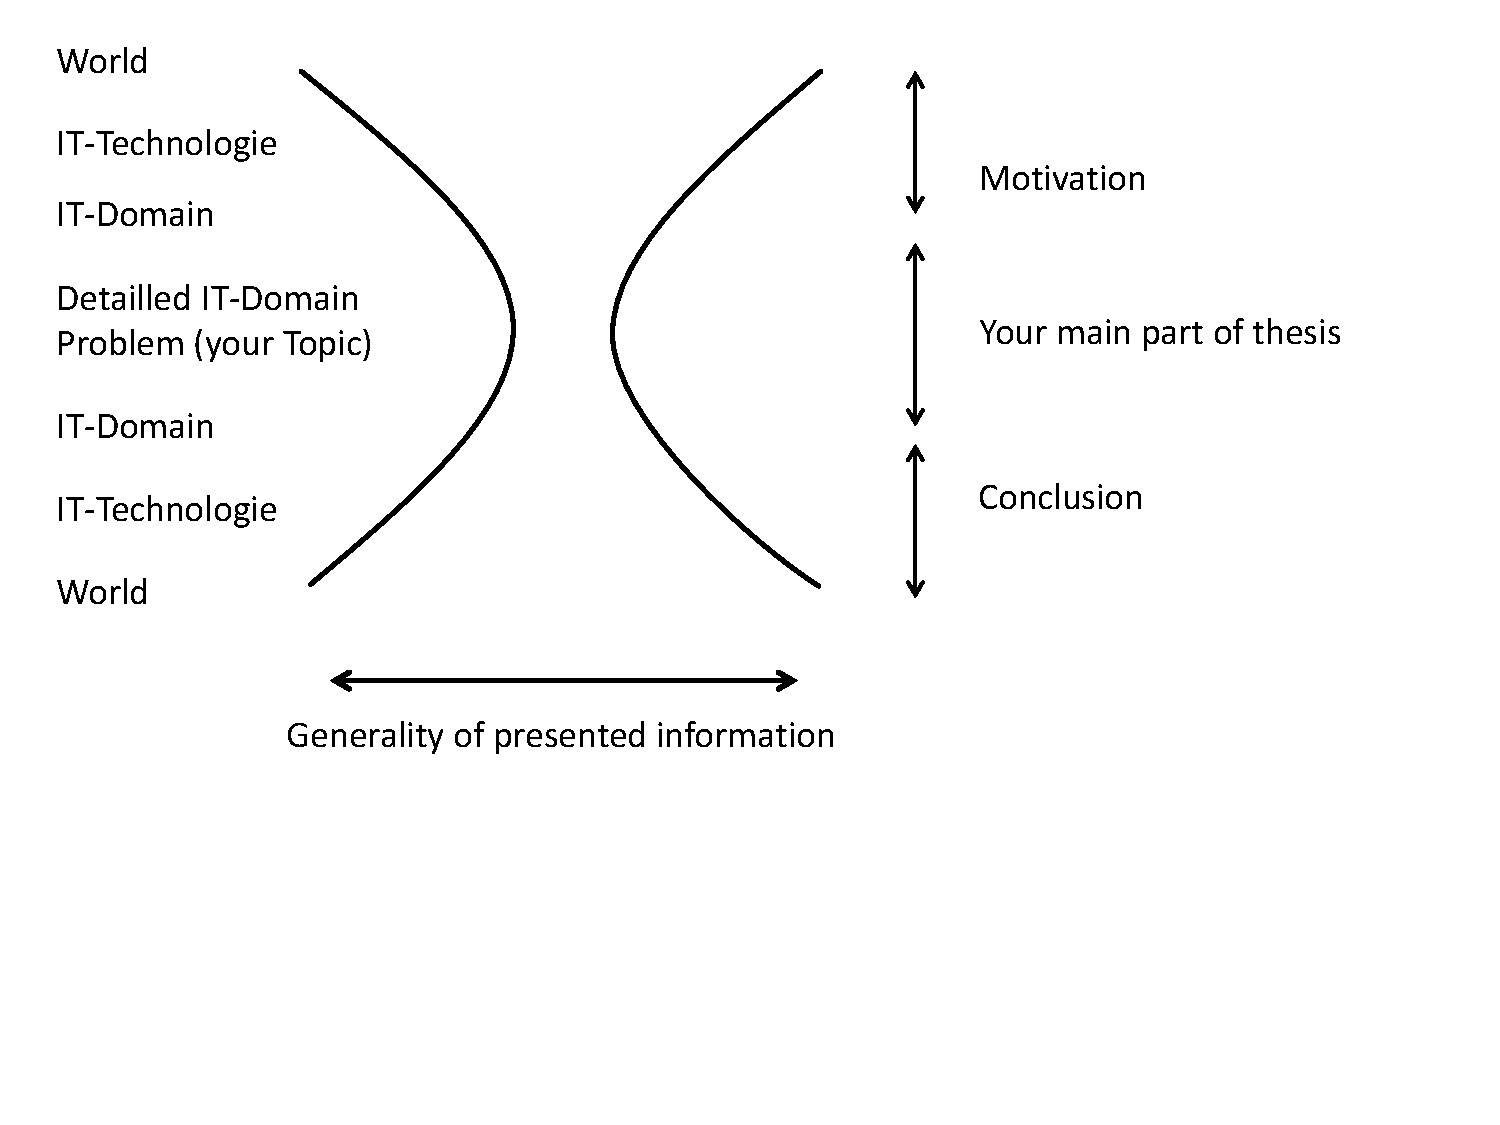
\includegraphics[width=0.9\textwidth]{template/writing}
%\caption[Information Generality]{This images illustrates how generality of information could be handled in a thesis. In your motivation you should start from a very broad view on the topic. Then you should get more precise with every statement until you reach the actual problem you are addressing. You should do vice-versa in your conclusion, starting with the problem that you addressed and getting broader until you can write about the meaning of your results to the (IT-)world.\label{fig:writing}}
%\end{figure}



Advances in drone technology in recent years
have opened the door to many civilian application possibilities,
especially in the commercial sector \cite{Dunn}.
Today, drones are already standard in 
aerial inspection services
\cite{Cohn, Equinox, Abuhasira}.
In the near future, the areas of
infrastructure,
transport,
insurance,
media and entertainment,
telecommunication,
agriculture,
safety
and mining 
are particularly promising for drones \cite{Mazur2016a}.
In contrast, 
genuine breakthroughs of more visionary applications, 
such as drone delivery or drone taxis,
are, if at all, only expected in the more distant future \cite{Rosen2019}.
Reasons for this are strict
regulations, skeptical public attitudes
and technical problems \cite{Rosen2019}.
Regarding the latter,
autonomous navigation methods are not yet 
robust enough for the reliable deployment in 
open-world environments of high uncertainty such as
densely populated urban areas \cite{brunner2019urban}.
This makes the autonomous navigation of drones
of great importance in current research.
Loquercio and Scaramuzza \cite{Loquercio2018a} 
categorize existing autonomous navigation methods for drones 
into classical methods and modern, machine learning based methods.

Classical autonomous navigation methods
follow the scheme of mapping-localization-planning-tracking.
Simpler approaches track pre-programmed waypoints based on GNSS
and are thus limited to flight environments that
first, have a reliable GNSS signal
(which often is not the case for 
urban areas, mountains, indoor sites, caves, etc.)
and second, are free of obstacles,
since functions to cope with them are absent.
More complex approaches use SLAM algorithms
to generate a map of the flight environment
and localize in it
based on the drone's visual or range sensors. \cite{MurArtal2015}
Path planning algorithms 
(e.g., \cite{Bircher2016}, \cite{Cieslewski2017})
apply to generate collision-free 
trajectories through the generated maps,
which are tracked
while estimating the drone state
based on data from the drone's inertial measurement unit (IMU)
and the output of SLAM algorithms 
(e.g., \cite{Lin2017}, \cite{Scaramuzza2014}, \cite{Sa2018}, \cite{Loianno2017}).
Theoretically, these approaches are deployable
in uncontrolled environments with unknown obstacles and other agents.
Practically, 
the mapping coerces global consistency,
which likely makes computations too complex 
for real-time execution onboard drones,
especially for non-static environments.

Modern autonomous navigation methods use machine learning
to replace the classical mapping-localization 
(or even the planning and tracking for more end-to-end methods) 
with the perception of the drone's onboard sensors
(e.g., camera, range, IMU)
and the decision-making of an ANN.
The way of learning further subdivides these methods into
reinforcement learning (RL) and imitation learning (IL) based methods.
In RL, the ANN learns with ``trial-and-error" \cite{Sadeghi2016}
from direct environmental interactions 
and thus avoids ``distributional mismatch" \cite{RobotAutonomy2}  
of training vs. testing, which is typical in IL.
However, this comes with the expense of a
substantially higher sample complexity 
compared to IL. \cite{Zhu2017}
This disadvantage is severe for drones because 
their limited flight endurance 
makes the learning process inefficient 
and collisions are uncontrolled and 
hence costly and dangerous. \cite{Sadeghi2016}

A popular research playground is autonomous drone racing
(e.g., \cite{Moon2019}, \cite{Jung2018}, \cite{Song2021})
because of the controlled flight environment,
the straightforward definition of goals
and the measurability and comparability of performance.
Methods for autonomous drone racing usually
integrate feedforward
convolutional neural networks (CNN) 
to map the current color or depth image to action
(e.g., \cite{RojasPerez2020}, \cite{Kaufmann2019}, \cite{Jung2018a}).
CNNs already achieve 
a high, spatial comprehension of how the drone's sensors perceive
the immediate environment.
However, this alone may not
be enough for the long-term objective of safely 
applying autonomous drones in open-world environments.
As humans are able to navigate safely there,
it seems promising to learn human-like abilities.
Temporal comprehension,
besides spatial comprehension,
has an important function in human navigation. 
For example, 
after entering a room through a door, 
a person can leave the room knowing 
that the door is behind him and 
does not need to keep the door in sight to do so.
Further, a person requires 
observing a sequence of images to
estimate the velocity and motion direction of herself or himself, 
obstacles or other agents.
In machine learning, recurrent neural networks
can establish temporal connections.
It is interesting to research the 
effect of using recurrent neural networks in autonomous drone racing.




%The controlled environment of autonomous drone racing 
%represents a convenient ground
%for basic research on autonomous navigation of drones
%because it clearly defines high-level goals, 
%i.e., to complete the racetrack,
%as well as intermediate goals, i.e., to fly through the next race gate.
%Moreover, the attainment of these goals can be intuitively assessed,
%for example, by considering the racetrack completion vs. the 
%maximum speed.





%The performance and robustness of different methods 
%can be assessed intuitively. 
%by means of 
%Moreover, several metrics to measure performance are provided,
%e.g., 
%
%high-level goals
%(i.e., completing the racetrack as fast/robust as possible)
%are defined and their 
%attainment can be measured (e.g., racetrack completions, flight time).
%Moreover, the racing environment is controlled
%and obsticles are known.

%Advanced methods for autonomous navigation of MAVs
%integrate feedforward, 
%deep convolutional neural networks (CNN)
%that, with a high spatial comprehension of the MAV's immediate surrounding, 
%map the current color or depth image to prediction or action.


%Consequently, 
%whether the state of the art in autonomous navigation of UAVs
%is sufficiently robust depends on the flight environment and the flight mission.
%Again, drone delivery provides an explanatory example here.
%Projects have been already 
%realized in rural areas where the airspace is mainly undisturbed [].
%Here, navigating through waypoints only relying on GNSS 
%without any implementation of obstacle avoidance and agent-coordination may be sufficient. 
%In contrast, urban areas are full of unstructered obstacles and other participating agents 
%which result in a high uncertainty that cannot be faced with in-advance planning. 
%Only a high level of autonomy in navigation
%could robustly cope with the challenges of this environment.
%This level has not yet been achieved.


%Research on autonomous MAV navigation mainly relies on deep learning 
%which allows to comprehend the immediate environment based on the perception of
%onboard sensors. \cite{loquercio2018learning}
%State-of-the-art navigation methods 
%achieve a high spatial understanding of the environment
%by feeding convolutional neural networks with RGB or depth data.
%This research aims to develop a simple navigation method 
%that extend this spatial perception onto temporal extension 
%by serially connecting a CNN with a long-short-term-memory (LSTM) network.
%Based on my assumption that powers of recall are crucial for humans when navigating,
%I am convinced that future autonomous navigation systems will also encompass this ability.
%The navigation method will be tested in simulation and real world in a simplified test scenario,
%which, however, requires the MAV to remember the expansion and relative motion of obstacles while considering its own elapsed acceleration.



%###################################################################################
%###################### Approach and Goals  ########################################
%###################################################################################
\section{Approach and Goals}
%DELETEME: 
%In this section, 
%you should cleary describe 
%your approach 
%that you are following 
%in order to solve 
%the underlaying problem 
%of your thesis. 
%Additionally, you should clearly state 
%the goals of your work. 
%This will not only help you supervizor 
%to understand what you are doing, 
%it will also help you to be sure 
%on which topic you should evaluate.



This thesis aims to 
investigate
whether temporal comprehension 
induced by a recurrent neural network
can be beneficial for
autonomous navigation in drone racing.
To do this, the thesis uses
the vision-based autonomous navigation method
proposed by Kaufmann et al. \cite{Kaufmann2018} as a baseline.
In the tests conducted by the authors, the baseline method
stood out from the compared methods
with high reliability and agility 
along dynamic flight curves through the racetrack.
The baseline method has a hybrid structure:
an artificial neural network 
inferring navigation decisions 
from the images of the drone's onboard camera
and a planning-control stack 
translating these decisions into flight movement.
The baseline ANN is a serial connection
of a convolutional neural network (CNN) 
and fully connected (FC) layers.
The CNN extracts visual features from imagery,
enabling the baseline method
to comprehend spatially what is in view of 
the drone's onboard camera.

This thesis extends the baseline ANN
with a multi-layer gated recurrent unit (GRU).
Theoretically, this
recurrent neural network variant 
enables the autonomous navigation method
to remember and to establish temporal connections.
Specifically, this means that navigation decisions 
base on both current and past sensor data.
Considering that, first, 
navigation can be seen as 
sequentially making decisions 
regarding how to move through space, and second, 
the thereby resulting trajectories 
are 4D objects in space and time, 
the CNN-GRU approach of this thesis, 
by incorporating both spatial and temporal understanding, 
likely improves race performance.
This thesis investigates this hypothesis in simulated drone races.
Different variants of ANNs 
are tested for their performance 
at different maximum speeds 
and for their ability to cope 
with intermediate target loss.
The latter refers to the event
that the next race gate leaves the FOV of the drone's camera
(e.g., because of a sharp turn between two race gates)
and the drone can only make meaningful navigation decisions
based on the memory induced by the GRU.







%According to the paper, the baseline has a success rate of 100 \% on the simulated racetrack when 
%the maximum speed is not greater than 9 m/s. For higher maximum speeds
%\{10, 11, 12\} m/s the success rate decreases to approximately \{85, 60, 35\} \%.
%Besides maximum speed, the simulated racetrack is designed in way that at any time the 
%currently targeted race gate is located in the frame of view (FOV) of the onboard camera.
%This is a requirement of the baseline because the CNN derives its navigation decisions only
%from the current image. In the event of intermediate target loss, i.e.,
%there is no race gate in the FOV and, consequently, on the image, the baseline 
%must result in undefined behaviour. 
%Intermediate target loss could for example 
%happen in the case of a steep curve between two consecutive race gates
%or in the case of an obstacle that temporally blocks the view to the currently targeted gate.
%In my thesis I plan to further develop only the first part of the hybrid approach.
%I intend to, first, replace the CNN with a R-CNN and,
%second, feeding additional features, i.e., data from the inertial measurement unit (IMU), to the network.
%The IMU data encompasses three (x, y, z) linear accelerations and three (x, y, z) angular velocities.
%I expect that thereby, 
%waypoints are not only generated on the basis of the current RGB image and IMU data, 
%but that also past sensor data is included in the navigation decision.
%This would possibly result in the following positive effects:
%\begin{itemize}
%	\item Making decisions on the basis of a series of sensor data makes the network more robust against outliers.
%			Otherwise, at high speeds, outliers may directly result in a crash.
%	\item Considering the similarity of recurrency to mathematical integration,
%			feeding IMU data to the network could have great potential since the network could be more or less able to internally estimate positions and orientations.
%	\item Due to its "memory", the network is able to generate meaningful waypoints in the case of intermediate target loss, i.e.,
%			the next gate of the race track is not depicted in the current image, but has appeared in previous images.
%	%\item Due to temporally distributed images, the network is able to take the speeds of moving gates (or obstacles) into the account of the navigation decisions.
%	\item Because trajectories are temporally extended maneuvers, a network with temporal comprehension is more able to imitate the expert system.
%			Thus, the resulting trajectory through the race track formed 
%			by the successively generated waypoints 
%			is more similar to a precomputed optimal trajectory.
%\end{itemize}
%The approach is implemented utilizing the middleware ROS \cite{ros}
%and simulated with the photo-realistic Flightmare Simulator \cite{song2020flightmare} built on Unity.
%For the implementation concept, see section \ref{sec:implConcept}.
%In simulation, the following tests should be conducted to compare my approach to the baseline.





%\paragraph{Randomized Figure-8 Drone Racing}
%Conduct test runs with increasing maximum speeds.
%For each run,
%build a randomized figure-8 drone racing track
%and test my approach and the baseline on the track.
%For each maximum speed, evaluate the percentage share of successful runs,
%the average time of racetrack completion
%and the
%closeness to the global trajectory in terms of optimality.
%The latter could be computed by recording the reference states
%that are continually pushed to the autopilot,
%taking the 4th derivative with respect to time (snap)
%and integrate the values.
%The in this way calculated cost could be used to measure closeness to
%the optimal, minimum snap global trajectory which the expert system used to generate the 
%training data.


%\paragraph{Intermediate target loss on sharp curve}
%Simulate two gates with a sharp curve in between.
%Before the drone passes the first gate,
%both successive gates must appear in the frame of view of the onboard camera.
%The curve must be so sharp, that, after traversing the first gate, not only the first but also the second gate has left the frame of view.
%The baseline, whose CNN makes navigation decisions from only the current image, will likely to fail in this scenario
%due to the absence of a goal.
%In contrast, my approach uses an R-CNN which is able to internally store information from previous images.
%In case that the R-CNN is well trained, it should be able to generate meaningful waypoints to complete the sharp curve and traverse the second gate.
%This becomes especially true, if the R-CNN is able to make use of the IMU data estimating poses.
%The percentage share of successful runs would be a convenient metric for evaluation.


%###################################################################################
%###################### Structure of the Thesis ####################################
%###################################################################################
\section{Structure of the Thesis}
%DELETEME: 
%This section does not require eloquent writing.
%It is just a presentation of what you will handle 
%in each chapter starting with Chapter~\ref{background}.

%DELETEME: Example: 
%This thesis is structured as follows. 
%In Chapter~\ref{background}, 
%we discuss essential background related to the thesis topic. 
%(SOME MORE SENTENCES). 
%Chapter~\ref{mainone} represents 
%a detailled analysis of the problem 
%that will be addressed. In particular, (SOME MORE SENTENCES). 
%In Chapter~\ref{maintwo}, 
%our solution is presented. 
%This solution covers ... (SOME MORE SENTENCES). 
%Chapter~\ref{evaluation} evaluates our solution 
%basing on our specified goals. 
%(SOME MORE SENTENCES). 
%In Chapter~\ref{conclusion}, we conclude. 
%Chapter~\ref{appendices} gives additional related information 
%on the topic of this thesis.



%DELETEME: Example: 
Chapter~\ref{background}
provides background information on the thesis topic,
including imitation learning with dataset aggregation
and the gated recurrent unit architecture.
Chapter~\ref{mainone} presents
the baseline autonomous navigation method
comprising the ANN module, 
the planning module, the control stack and the expert system.
Special attention is paid to the ANN module,
which extends the baseline ANN with the temporal comprehension of the GRU.
Chapter~\ref{maintwo} presents the design of the
experiments conducted in this thesis,
including the simulation setup,
the imitation learning process and the race tests.
Chapter~\ref{evaluation} evaluates 
the experimental results
focussing on the impact of temporal comprehension on performance.
Chapter~\ref{conclusion} concludes this thesis. 
Chapter~\ref{appendices} provides additional related information.
\chapter{Background}
%labels will help you to reference to certain images, tables, chapters, section, and so on...
\label{background}

%DELETEME: This chapter will cover all of your background information and related work. Background and related work are directly related to your thesis. Please do not place irrelevant content here which is a common mistake. Citing will be handled in the appendices.
%
%DELETEME: Background represents underlaying knowledge that is required to understand your work. The expected knowledge level of your readers can be set to the one of a bachelor or master student who just finished his studies (depending on what kind of thesis you are writing). This means that you do not need to describe how computers work, unless your thesis topic is about this. Everything that an avarage alumni from your field of studies should now does not need to be described. It turn, background information that is very complex and content-wise very near to you problem, can be placed in the main parts. Everyting else should be written here. Note: it is important to connect each presented topic to your thesis. E.g. if you present the ISO/OSI layer model you should also write that this is needed to understand the protocols you plan to develop in the main parts.
%
%DELETEME: Related work respresents results from work that handled the same or a similar problem that you are addressing. This work might have used a different approach or might not have been that successful. Finding a paper / work that solved your problem in the same way you were planning to do is not good and you should contact your supervizor for solving this issue. Again, each paper / work has to be connected to your approach: other papers might have not chosen an optimal solution; they might not have been taking care of essential aspects; they might have chosen a different approach and you believe, yours will work better ...

%###################################################################################
%###################### Topic A             ########################################
%###################################################################################
%\section{Topic 1}

%###################################################################################
%###################### Topic B             ########################################
%###################################################################################
\section{Imitation Learning with Dataset Aggregation} \label{sec:imitation_learning}

\newcommand{\parentheses}[1]{\left({#1}\right)}
\newcommand{\brackets}[1]{\left[{#1}\right]}
\newcommand{\braces}[1]{\left\{{#1}\right\}}

\newcommand{\timestep}{t}
\newcommand{\state}{\underline{x}}
\newcommand{\stateDomain}{\mathcal{X}}
\newcommand{\action}{\underline{u}}
\newcommand{\actionDomain}{\mathcal{U}}
\newcommand{\probability}{p}

\newcommand{\policy}{\pi}
\newcommand{\demonstration}{\xi}
\newcommand{\expertt}{*}
\newcommand{\parameterVector}{\underline{\theta}}
\newcommand{\trajectory}{\tau}

This section first, defines the general imitation learning problem, 
second, presents behavioral cloning as the simplest form of direct policy learning 
and third, introduces the more sophisticated direct policy learning method 
of dataset aggregation, 
which was originally proposed as DAgger by Ross et al. \cite{Ross2010}.
The experiments of this thesis (see chapter \ref{mainone}) 
dataset aggregation to the imitation learning problem 
of the ANN module in the autonomous navigation method (see chapter \ref{maintwo}). 



Imitation learning is an area of machine learning 
that considers the task of learning to
imitate (i.e., behave like) an expert 
in a sequential decision-making problem \cite{yue2018imitation}.
It applies naturally to learning problems where it is easier 
to demonstrate the desired behavior of how to attain a goal
than to define intermediate goals and rewards 
(as in supervised and reinforcement learning, respectively)
that lead to the desired behavior \cite{Nikolov2018}.
In terms of supervision,
imitation learning is therefore
between supervised learning
and reinforcement learning.
Imitation learning performs well in tasks
related to human intent or behavior, e.g.,
pedestrian avoidance \cite{Ziebart2009},
speech animation \cite{Taylor2017},
sport analytics \cite{le2017data}
and gaming \cite{thurau2004imitation}.
Regarding
planning and control
in autonomous navigation,
imitation learning has become 
state-of-the-art \cite{Mero2022}.
According to their approach, 
imitation learning methods 
divide into direct policy learning and 
inverse reinforcement learning \cite{RobotAutonomy2}.
Direct policy learning 
optimizes a policy class 
to approximate the expert's behavior
by reducing the imitation learning problem
to a single or a sequence of supervised learning problems.
Inverse reinforcement learning
optimizes a reward function 
to approximate the expert's underlying intent
and deploys reinforcement learning methods
to optimize a policy class to maximize the identified reward. 







\paragraph*{Problem Definition}$\ $\\
An imitation learning problem includes: 
a system, 
an expert, 
a policy class, 
a loss function, 
and a learning algorithm \cite{yue2018imitation}.
The goal is to find the policy 
within the policy class 
that approximates the expert's decision-making 
on the system's actions
as closely as possible. 

The system interacts with its real or simulated environment.
At time step $\timestep$,
the system is in the state $\state_\timestep \in \stateDomain$
and executes the action $\action_\timestep \in \actionDomain$
where $\stateDomain$ and $\actionDomain$ are the 
spaces of all existing system states and actions, respectively.
The system is considered a Markov decision process
whose initial state is randomly distributed 
%$\probability \parentheses{\state_0}$
\cite{RobotAutonomy2}.
Thus, a probabilistic transition model can 
describe the system dynamics 
providing the conditional probability distribution 
over the system state 
given the system state and action from the previous time step
\begin{align}
    \probability \parentheses{
        \state_\timestep | \state_{\timestep -1}, \action_{\timestep -1}
    }.
\end{align}

%Note that the explicit system dynamics are typically unknown 
%for the policy class to be trained.

The expert 
%(also referred to as demonstrator)
is a human or a computer program 
that makes state-based action decisions,
which cause the system to act as desired.
The expert policy, which maps system states to expert actions, 
represents the expert's decision-making process
\begin{align}
    \policy^\expertt
    :\ \stateDomain \rightarrow \actionDomain
    ;\quad 
    \state_\timestep 
    \mapsto 
    \action_\timestep^\expertt
    %\policy^\expertt\parentheses{\state_\timestep}
    .
\end{align}
Applying the expert policy on a system state
yields a demonstration,
i.e., a state-action pair 
$\parentheses{\state_\timestep, \action_\timestep^\expertt}$.


The policy class defines the search space for
finding the optimal policy, i.e., 
the policy that most closely resembles the expert policy.
Usually, 
the policy class is an ANN
\begin{equation}
    \policy_{\parameterVector}
    :\ \stateDomain \rightarrow \actionDomain
    ;\quad \state_\timestep \mapsto 
    \policy_{\parameterVector} \parentheses{\state_\timestep}
\end{equation}
where the vector $\parameterVector$ 
contains the trainable parameters of the ANN.

Both, the expert policy 
and members of the policy class, can roll out.
%Rolling out the expert policy
%yields a trajectory of demonstrations
%$\trajectory = \parentheses{\state_\timestep, \action_\timestep^\expertt}
%_{\timestep \in \braces{0, 1, \dots}}$.
The rollout of a general policy 
$\policy :\ \stateDomain \rightarrow \actionDomain$
denotes the process, 
in which the system, 
starting from the initial state 
$\state_0 \sim \probability \parentheses{\state_0}$,
interacts with the environment 
based on the actions inferred by that policy
for a certain number of time steps
\begin{align}
    \probability \parentheses{
        \state_\timestep | \state_{\timestep -1}, \policy\parentheses{\state_{\timestep-1}}
    },\ \timestep \in \braces{0,\dots, T}.
\end{align}
A rollout produces a trajectory,
which is the sequence of the state-action pairs visited during rollout
\begin{align}
    \trajectory = \parentheses{\state_\timestep, 
    \policy\parentheses{\state_\timestep}}
    _{\timestep \in \braces{0, \dots, T}}.    
\end{align}
The policy induces the state distribution of a rollout, i.e., the probability that the system visits a state, which would therewith become part of the rollout trajectory. The rollout state distribution is the average of the state distributions over the time steps of the rollout.
\begin{equation}
    \probability \parentheses{\state | \policy}
    = \frac{1}{T+1} \sum_{\timestep = 0}^T
    \probability \parentheses{\state_\timestep | \policy}.
\end{equation}


%Multiple expert trajectories constitute a training dataset
%%on which the policy class can be trained
%\begin{align}
%    D = \braces{\trajectory_i}_{i \in \braces{1, 2, \dots}}.
%\end{align}


%The rollout of a member of the policy class also produces
%a trajectory ...
%The policy class can be rolled out, i.e.,
%to repeatedly apply the policy on an inital state.
%Thereby, it generates the trajectory 
%\begin{align}
%    \tau = \braces{
%        \parentheses{\state_\timestep, \policy \parentheses{\state_\timestep}}
%    }_{\timestep \in \braces{0, 1, \dots}}
%    .
%\end{align}
The loss function measures
how much an action 
predicted by a policy for a system state
deviates
from the action demonstrated by the expert for the same state
\begin{align}
    L_{\policy}
    :\ \stateDomain \rightarrow \mathbb{R}
    ;\quad
    \state_\timestep
    \mapsto
    L_{\policy}
    \parentheses{
        \policy\parentheses{\state_\timestep},
        \policy^\expertt\parentheses{\state_\timestep}
    }.
\end{align}
Applied on a set of demonstrations,
the loss function quantifies how closely a policy
imitates the expert policy. 



%The learning algorithm 
%finds the policy $\hat{\policy}^\expertt$ 
%within the policy class 
%that is closest to the expert policy. 
%For this purpose, the algorithm 
%minimizes the total imitation loss 
%evaluated on states sampled 
%from the distribution 
%induced by the identified policy itself.
%In machine learning, 
%this corresponds to the training of the ANN, 
%whereby the algorithm updates the trainable parameters of the ANN 
%in accordance to the evaluated loss

The learning algorithm searches for the optimal policy 
$\hat{\policy}^\expertt$
within the policy class by minimizing the total imitation loss, 
whereby the state distribution of the loss evaluation 
is equal to the distribution when rolling out the optimal policy.
As a result, the state distributions at learning and test rollouts 
do not differ, which ensures that low training losses 
transfer to high test performances.
In machine learning, this corresponds to the training of the ANN, 
in which the algorithm updates the trainable parameters of the ANN 
in accordance to the evaluated loss
\begin{equation}
    \hat{\policy}^\expertt
    =
    \argmin{\parameterVector}
    \sum_{
        \state \sim \probability \parentheses{
            \state | \policy_{\parameterVector}}
    }
    L_{\policy_{\parameterVector}} \parentheses{\state}
    %L \parentheses{
    %    \policy_{\parameterVector}\parentheses{\state_\timestep},
    %    \policy^\expertt\parentheses{\state_\timestep}
    %}
    .
\end{equation}
The above optimization is a 
``non-i.i.d. supervised learning problem" \cite{Ross2010}. 
As the system dynamics are unknown or too complex, 
training data can only be collected in rollouts. 
Thereby, the distribution of the training data is induced 
by the rolled out policy and hence 
neither independent and identically distributed (i.i.d.) 
across the system state space $\stateDomain$ 
nor equal to the distribution 
induced by the optimal policy yet unknown. 
Because of the interdependence of policies and training data distributions, 
closing the ``distributional mismatch" \cite{RobotAutonomy2} 
is a non-convex optimization problem, 
which is significantly more difficult and time-consuming 
than common supervised learning.





\paragraph*{Behavioral Cloning}$\ $\\
Behavioral cloning reduces the imitation learning problem 
to a single, convex supervised learning problem 
on a pre-collected training dataset 
of expert trajectories, where each trajectory is the product of an 
expert policy rollout and 
contains the thereby demonstrated state-action pairs
\begin{equation}
    D = \braces{\trajectory_i^\expertt}_{i \in \braces{1, 2, \dots}}
    ,\quad
    \trajectory_i^\expertt = \parentheses{
        \state_{i,\timestep}, \action_{i,\timestep}^\expertt}
    _{\timestep \in \braces{0, 1, \dots}}.
\end{equation}
The optimization problem of behavioral cloning
is to minimize the 
total imitation loss on the demonstrations
$\parentheses{\state_\timestep, \action_\timestep^\expertt}$ 
in the trajectories 
$\trajectory_i$
of the pre-collected dataset $D$
\begin{align}
    \hat{\policy}^\expertt
    &=
    \argmin{\parameterVector}
    \sum_{\trajectory_i \in D} \quad
    \sum_{\parentheses{\state_\timestep, \action_\timestep^\expertt} \in \trajectory_i
    }
    L \parentheses{
        \policy_{\parameterVector} \parentheses{\state_\timestep},
        \action_\timestep^\expertt
    }
    \nonumber\\ &=
    \argmin{\parameterVector}
    \sum_{
        \state \sim \probability \parentheses{
            \state | \policy^\expertt}
    }
    L_{\policy_{\parameterVector}} \parentheses{\state}
    ,
\end{align}
given the expert rollout state distribution
\begin{equation}
    \probability \parentheses{\state | \policy^\expertt}
    = \frac{1}{T+1} \sum_{\timestep = 0}^T
    \probability \parentheses{\state_\timestep | \policy^\expertt}.
\end{equation}
Compared to general imitation learning, behavioral cloning 
generally exhibits different distributions at training and testing
\begin{equation}
    \probability \parentheses{\state | \policy^\expertt}
    \neq 
    \probability \parentheses{\state | \policy_{\parameterVector}}.
\end{equation}
This plus the fact that the training data is 
generally not i.i.d. across the state space 
makes it likely that the ANN, when rolling out, 
faces states not seen during training. 
As a result, low training losses do not guarantee high test performances. 
This is especially true for a longer rollouts 
because the upper bound of the error grows quadratically 
with the number of time steps $T$ \cite{yue2018imitation}. 
Although the above optimization minimizes 
the one-step loss of the ANN along the expert trajectories, 
when the ANN rolls out, these one-step errors accumulate 
along the ANN trajectory and will very likely 
cause non-negligible deviations from the expert trajectories 
of the training dataset.




\paragraph*{Dataset Aggregation}$\ $\\
Dataset aggregation (originally proposed as DAgger \cite{Ross2010}) 
extends behavioral cloning iteratively.
It reduces the imitation learning problem 
to a sequence of convex supervised learning problems.
The fundamental concept of the method takes the following steps.
\begin{enumerate}
    \item 
    Roll out the expert policy $\policy^\expertt$,
    record the thereby resulting trajectory
    and initialize the aggregated dataset with that trajectory
    $D_0 = \trajectory_0$.
    Train the ANN with supervised learning on the aggregated dataset
    to receive
    $\policy_{\parameterVector, 0}$.
    \item Until the ANN exhibits the desired behavior when rolling out, 
    do for iteration $i = 1,2,\dots$
    \begin{enumerate}
        \item Rollout the ANN from the last training
        $\policy_{\parameterVector, i-1}$
        and record the thereby visited states
        $\parentheses{\state_{i,\timestep}}_{t\in \braces{0, \dots, T_i}}$.
        \item Apply the expert policy to the recorded states 
        to receive a trajectory of demonstrations
        $\trajectory_i = \parentheses{\state_{i,\timestep}, 
    \policy^\expertt\parentheses{\state_{i,\timestep}}}
    _{\timestep \in \braces{0, \dots, T_i}}$.
        \item Add the labeled trajectory to the aggregated dataset
        $D_i = D_{i-1} \cup \trajectory_i$.
        \item Train the ANN with supervised learning on the aggregated dataset
        to receive
        $\policy_{\parameterVector, i}$.
    \end{enumerate}
\end{enumerate}
In contrast to behavioral cloning,
dataset aggregation requires first, 
access to the system for executing ANN rollouts
and second, 
an interactive expert providing feedback 
on the thereby visited states \cite{yue2018imitation}.
In the iterative learning process,
dataset aggregation
remembers and confronts the ANN with
its mistakes made in rollouts corrected by the expert.
Ideally, this procedure reduces the 
state distribution differences between learning and rollouts
to the point where
the trainable parameters of the ANN converge to their
optimal values for the general imitation learning problem.





%###################################################################################
%###################### Topic C             ########################################
%###################################################################################
\section{Gated Recurrent Unit} \label{sec:gru}
In this thesis,
the ANN module of the autonomous navigation method (see section \ref{mainone})
is extended with the gated recurrent unit (GRU), 
which is a special recurrent neural network (RNN) architecture
proposed by Cho et al. \cite{Cho2014},
with the aim to involve temporal comprehension in
the navigation decision-making.
This section introduces the class of RNNs
and relates the GRU to standard RNNs
and the more prevalent long short-term memory (LSTM).
Moreover, it provides information regarding first,
the state and gating mechanisms that make the GRU able to comprehend temporally at inference
and second, how the GRU learns with backpropagation through time.

\paragraph*{Recurrent Neural Networks} ${}$\\
RNNs contrasts with classical feedforward ANNs, 
which forward information only towards subsequent layers, 
by featuring dynamic properties that stem 
from implementing feedback connections
\cite{Hu2008} (see fig. \ref{fig:rnn_folded}).
As previously inferred states re-enter the network, 
the output of an RNN depends not only on the current 
but also on prior inputs. 
In this sense, RNNs are qualified to process and infer from 
entire sequences of data points. 
In the case of time-series data, 
this equates to temporal comprehension and memory \cite{ICE2020}.
RNNs train on sequential data with backpropagation through time (BPTT) 
\cite{pascanu2013difficulty}
which is basically the application of standard backpropagation
(e.g., \cite{Rojas1996})
on the unfolded representation of an RNN
(see fig. \ref{fig:rnn_unfolded}).
This representation exhibits a layer 
for each data point in the processed input sequence 
and is construable as a feedforward ANN 
that shares its trainable parameters across its layers. 
The longer the input sequences,
the deeper the unfolded representation of an RNN becomes. 
The training of RNNs on long input sequences 
is hence prone to the 
vanishing gradient problem \cite{hochreiter1991untersuchungen},
which slows down or ceases the convergence 
of the trainable parameters of the RNN.
As a result, standard RNNs have difficulties 
learning to connect to information deep in the past \cite{Bengio1994}.
\begin{figure}[h]
    \centering
    \subfloat[
        Folded
    ]{
        \label{fig:rnn_folded}
        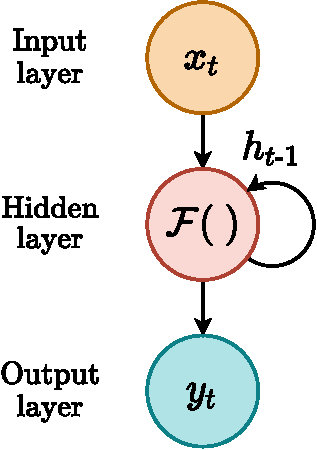
\includegraphics[height=0.35\textwidth]{own/rnn_folded.drawio.pdf}
    }
    \hspace*{2cm}                
    \subfloat[
        Unfolded
    ]{
        \label{fig:rnn_unfolded}
        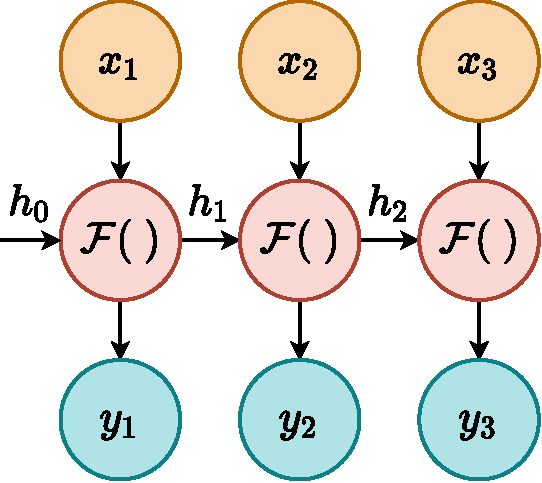
\includegraphics[height=0.35\textwidth]{own/rnn_unfolded.drawio.pdf}
    }
    \caption[
        Folded and unfolded RNN
    ]{
        Folded representation of an RNN with a single hidden layer 
        inferring $y_t = \mathcal{F}\left(x_t, h_{t-1}\right)$ from the current input
        and the previous hidden state
        and the time-unfolded representation
        when processing the input sequence
        $\left(x_i\right)_{i\in\{1, 2, 3\}}$.
        \label{fig:rnn_folded_unfolded}
    }
\end{figure}




In 1997, Hochreiter and Schmidhuber \cite{Hochreiter1997} 
introduced the long short-term memory (LSTM), 
which is today's predominant RNN architecture \cite{schmidhuber_2021}. 
A standard LSTM layer
recurrently maintains a cell state and a hidden state. 
This means that, besides the current data point of the input sequence, 
the layer re-inputs the fed back cell state and hidden state 
from the previous sequential step. 
Furthermore, the LSTM layer implements three gating mechanisms 
to control the information flow within the layer. 
A gating mechanism is basically the Hadamard product 
of a state and a gate, 
which is a vector whose entries are within the interval from zero to one. 
Consequently, a gate applied to a state controls the flow 
of the state elements within the range from zero to full flow. 
The forget gate of the LSTM layer controls the flow 
from the previous to the current cell state. 
The input gate controls the flow from the previous hidden state 
and the current data point of the input sequence 
to the current cell state. 
And the output gate controls the flow from the current cell state 
to the current hidden state. 
By this design of recurrent states with gated information flow, 
the training of the LSTM is essentially robust 
to the vanishing gradient problem \cite{pascanu2013difficulty}. 
As a result, the LSTM is, compared to standard RNNs, 
more capable of learning to remember long-term dependencies 
within input sequences.


The GRU, which was proposed 17 years after the LSTM by 
Cho et al. \cite{Cho2014}, 
is a lighter version of the LSTM. 
It refrains from the cell state and therewith the output gate of the LSTM 
and only has a hidden state and two gating mechanisms. 
Therewith, the GRU has less trainable parameters 
than the LSTM and is less memory efficient. 
Nevertheless, it preserves the robustness towards 
the vanishing gradient problem \cite{ICE2020}. 
Various empirical studies compared the GRU and the LSTM. 
Greff et al. \cite{Greff2017} found no substantial performance 
differences between the GRU and several LSTM variants 
in speech and handwritten text recognition and music representation. 
Chung et al. \cite{Chung2014} detected an equally well performance 
of the GRU and the LSTM processing raw speech and polyphonic music data. 
In the comparative study of Yin et al. \cite{Yin2017}, 
the GRU slightly outperforms the LSTM 
in five of seven natural language processing tasks. 
Kaiser and Sutskever \cite{Kaiser2015} achieved better 
results with a GRU-based than with an LSTM-based network 
in algorithm learning. 
Considering the above findings and the lower complexity, 
this thesis uses the GRU and not the LSTM 
for the ANN module of the autonomous navigation method.




\paragraph*{Inference}$\ $\\
The following presents the mathematics 
of the inference
of a single GRU layer
in accordance with the PyTorch implementation\footnote{
    \url{https://pytorch.org/docs/stable/generated/torch.nn.GRU.html}, accessed on \today
}.
This includes the layer's two gating mechanisms
and its computations of the candidate state and the hidden state.






Without loss of generality,
let the sequential data to be processed by the GRU layer
be a batch of time series of data points
\begin{equation}
    \left(
        \underline x_t
        \in \mathbb{R}^{N^\text{in}}
    \right)_{
        t \in \left\{
            1, \dots, N^\text{seq}
        \right\}
        ,
        i
    }
    ,\quad
    i \in \left\{
        1, \dots, N^\text{batch}
    \right\},
\end{equation}
where $N^\text{batch}$ is the batch size, 
$N^\text{seq}$ is the sequence length 
and $N^\text{in}$ is the dimensionality of the data points.
Let the initial batch of hidden states be
\begin{equation} \label{eq:gru_init_hidden_state}
    \underline h_{0,i}
    \in \left[-1, 1\right]^{N^\text{hidden}}
    ,\quad
    i \in \left\{
        1, \dots, N^\text{batch}
    \right\},
\end{equation}
where $N^\text{hidden}$ is the dimensionality
of the hidden state, which is a design parameter of the GRU layer.
The values of the initial hidden states $\underline h_{0,i}$
are typically zero or noisy \cite{Zimmermann2012}
but can also be learned (e.g., \cite{Forcada1995}).
The GRU layer processes the time series included in the batch parallelly 
and the data points of the individual time series successively.
At the current time step $t$,
the layer's input comprises 
the batch of the current data points
and the fed back batch of previously outputted, hidden states
\begin{equation}
    \left(
    \underline x_{t,i}
    ,\ 
    \underline h_{t-1,i}
    \right)
    ,\quad
    i \in \left\{
        1, \dots, N^\text{batch}
    \right\}.
\end{equation}
For simplification, the following text only refers 
to the parallelly computed, individual elements of the processed batch. 
However, the following equations yet explicitly refer to the entire batch.


At every incoming input, the GRU layer initially computes its two gates. 
The current reset gate 
\begin{equation}
    \underline g^\text{r}_{t,i} 
    =
    \mathcal{F}^\text{r} \left( \underline x_{t,i}, \underline h_{t-1,i}\right)
    ,\quad i \in \left\{1, \dots, N^\text{batch}\right\}
\end{equation}
results from the map
\begin{align} \label{eq:gru_reset}
    \mathcal{F}^\text{r}
    &:
    \left(\mathbb{R}^{N^\text{in}},\ \left[-1, 1\right]^{N^\text{hidden}}\right)
    \rightarrow
    \left[0, 1\right]^{N^\text{hidden}}
    \nonumber \\ & \quad
    \left(\underline x,\underline h\right)
    \mapsto
    \hadfct{\sigma} \left(
        \underline{\underline A}^\text{r}_{x} \underline x
        +
        \underline b^\text{r}_{x}
        +
        \underline{\underline A}^\text{r}_{h} \underline h
        +
        \underline b^\text{r}_{h}
    \right).
\end{align}
The above map to the reset gate comprises two steps. 
First, it linearly transforms the current data point 
and the previous hidden state 
with the trainable weight matrices and bias vectors
\begin{align} \label{eq:gru_reset_params}
    \underline{\underline A}^\text{r}_{x} & \in \mathbb{R}^{
        N^\text{hidden}
        \times
        N^\text{in}
    },
    & \underline{b}^\text{r}_{x} & \in \mathbb{R}^{N^\text{hidden}},
    \nonumber \\
    \underline{\underline A}^\text{r}_{h} & \in \mathbb{R}^{
        N^\text{hidden}
        \times
        N^\text{hidden}
    },
    & \underline{b}^\text{r}_{h} & \in \mathbb{R}^{N^\text{hidden}},
\end{align}
whereby the user has the design option to disable all biases of the GRU layer.
This is tantamount to set the above and the below biases of the layer to zero 
and consider them not trainable.
Second, the standard sigmoid function \cite{Han1995} 
(see fig. \ref{fig:gru_activations})
\begin{equation} \label{eq:sigmoid}
    \sigma :\ 
    \mathbb{R} \rightarrow \left[0,1\right] ;\ 
    x \mapsto \frac{1}{1 + e^{-x}}
\end{equation}
applies element-wise (denoted with the accent $\odot$) 
to the sum of these two linear transformations.
The sigmoid function limits the values of the reset gate 
to the interval between zero and one. 
This is characteristic of a gating mechanism, 
which targets at only damping, 
not amplifying or reversing the individual values of the state.

The current update gate 
\begin{equation}
    \underline g^\text{u}_{t,i} 
    =
    \mathcal{F}^\text{u} \left( \underline x_{t,i}, \underline h_{t-1,i}\right)
    ,\quad i \in \left\{1, \dots, N^\text{batch}\right\}
\end{equation}
results from the map
\begin{align} \label{eq:gru_update}
    \mathcal{F}^\text{u}
    &:
    \left(\mathbb{R}^{N^\text{in}},\ \left[-1, 1\right]^{N^\text{hidden}}\right)
    \rightarrow
    \left[0, 1\right]^{N^\text{hidden}}
    \nonumber \\ & \quad
    \left(\underline x,\underline h\right)
    \mapsto
    \hadfct{\sigma} \left(
        \underline{\underline A}^\text{u}_{x} \underline x
        +
        \underline b^\text{u}_{x}
        +
        \underline{\underline A}^\text{u}_{h} \underline h
        +
        \underline b^\text{u}_{h}
    \right).
\end{align}
The above map to the update gate is the same 
as the map to the reset gate but has 
its own trainable weight matrices and bias vectors
\begin{align} \label{eq:gru_update_params}
    \underline{\underline A}^\text{u}_{x} & \in \mathbb{R}^{
        N^\text{hidden}
        \times
        N^\text{in}
    },
    & \underline{b}^\text{u}_{x} & \in \mathbb{R}^{N^\text{hidden}},
    \nonumber \\
    \underline{\underline A}^\text{u}_{h} & \in \mathbb{R}^{
        N^\text{hidden}
        \times
        N^\text{hidden}
    },
    & \underline{b}^\text{u}_{h} & \in \mathbb{R}^{N^\text{hidden}}.
\end{align}

Knowing the current reset gate, the GRU layer computes the candidate state
\begin{equation}
    h^\text{c}_{t,i}
    =
    \mathcal{F}^\text{c} \left( \underline x_{t,i}, \underline h_{t-1,i}\right)
    ,\quad i \in \left\{1, \dots, N^\text{batch}\right\}
\end{equation}
with the map
\begin{align} \label{eq:gru_candidate}
    \mathcal{F}^\text{c}
    &:
    \left(
        \mathbb{R}^{N^\text{in}}, \left[-1, 1\right]^{N^\text{hidden}}
    \right)
    \rightarrow
    \left[-1, 1\right]^{N^\text{hidden}}
    \nonumber \\ & \quad
    \left(\underline x, \underline h \right)
    \mapsto
    \hadfct{\tanh} \left[
        \underline{\underline A}^\text{c}_{x}
        \underline x
        +
        \underline b^\text{c}_{x}
        +
        \mathcal{F}^\text{r} \left(\underline x, \underline h \right)
        \odot
        \left(
            \underline{\underline A}^\text{c}_{h}
            \underline h
            +
            \underline b^\text{c}_{h}
        \right)
    \right],
\end{align}
which has the trainable weight matrices and bias vectors
\begin{align} \label{eq:gru_candidate_params}
    \underline{\underline A}^\text{c}_{x} & \in \mathbb{R}^{
        N^\text{hidden}
        \times
        N^\text{in}
    },
    & \underline{b}^\text{c}_{x} & \in \mathbb{R}^{N^\text{hidden}},
    \nonumber \\
    \underline{\underline A}^\text{c}_{h} & \in \mathbb{R}^{
        N^\text{hidden}
        \times
        N^\text{hidden}
    },
    & \underline{b}^\text{c}_{h} & \in \mathbb{R}^{N^\text{hidden}}.
\end{align}
The above map to the candidate state 
resembles the maps to the reset and the update gate 
by subjecting the current data point and the previous hidden state 
to a separate, biased linear transformation, 
but differs in two aspects. 
First, before adding the results of the two transformations, 
the current reset gate applies to the transformed, previous hidden state 
($\odot$ denotes the Hadamard product).
Thereby, the reset gate mitigates the contribution 
of the previous hidden state to the candidate state. 
Second, instead of the sigmoid function, 
the hyperbolic tangent \cite{D.1966} (see fig. \ref{fig:gru_activations})
\begin{equation} \label{eq:tanh}
    \tanh
    :\ 
    \mathbb{R}
    \rightarrow
    \left[
        -1,1
    \right]
    ;\ 
    x 
    \mapsto 
    \frac{
        e^x - e^{-x}
    }{
        e^x + e^{-x}
    }
\end{equation}
applies element-wise to the sum of the transformed data point 
and the gated, transformed, previous hidden state, 
which limits the values of the candidate state 
to the interval from minus to plus one.



Finally, the GRU layer computes the current hidden state
\begin{equation} \label{eq:gru_layer_current_hidden}
    h_{t,i}
    =
    \mathcal{F}^\text{h} \left( \underline x_{t,i}, \underline h_{t-1,i}\right)
    ,\quad i \in \left\{1, \dots, N^\text{batch}\right\}
\end{equation}
with the map
\begin{align} \label{eq:gru_layer_map_hidden}
    \mathcal{F}^\text{h}
    &:
    \left(
        \mathbb{R}^{N^\text{in}}
        ,\ 
        \left[-1, 1\right]^{N^\text{hidden}}
    \right)
    \rightarrow
    \left[-1, 1\right]^{N^\text{hidden}}
    \nonumber \\ & \quad
    \chi := \left(
        \underline x
        ,\ 
        \underline h
    \right)
    \mapsto 
    %\dots \nonumber \\ & \qquad \qquad \dots
    \left[
        \underline 1 
        -
        \mathcal{F}^\text{u}\left(\chi\right)
    \right]
    \odot
    \mathcal{F}^\text{c} \left(\chi\right)
    +
    \mathcal{F}^\text{u}\left(\chi\right)
    \odot
    \underline h
    .
\end{align}
The above map to the hidden state is a weighted arithmetic mean 
of the previous hidden state and the current candidate state, 
where the current update gate and its counter gate are the weights. 
Therewith, the update gate controls the element-wise percentages 
of the two states in the current hidden state. 
The fact that the hyperbolic tangent normalizes the elements 
of the candidate state to the interval from minus to plus one 
(see equ. \ref{eq:gru_candidate})
limits the values of the current hidden state to the same interval 
(given that the values of initial hidden state
(equ. \ref{eq:gru_init_hidden_state})
are also in that interval).
\begin{figure}
    \centering
    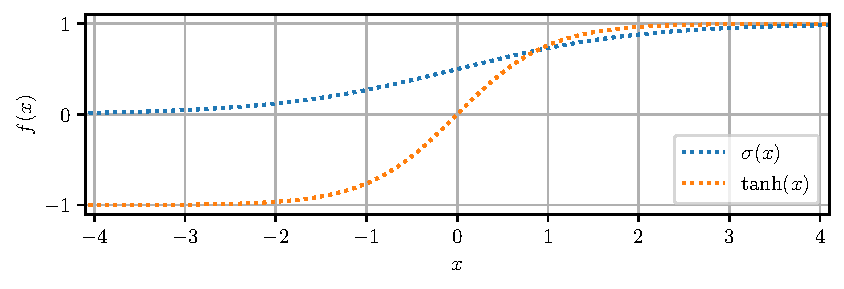
\includegraphics[width=0.9\textwidth]{own/sigmoid_tanh.pdf}
    \caption[
        Activation functions of the GRU
    ]{
        Activation functions of the GRU.
        The standard sigmoid function
        (see equ. \ref{eq:sigmoid})
        normalizes the values
        of the reset and the update
        gate to the interval from zero to one
        (see equ. \ref{eq:gru_reset} and \ref{eq:gru_update}).
        The hyperbolic tangent
        (see equ. \ref{eq:tanh})
        normalizes the values 
        of the candidate
        and therewith the hidden state 
        to the interval from minus to plus one
        (see equ. \ref{eq:gru_candidate} and \ref{eq:gru_layer_map_hidden}).
        \label{fig:gru_activations}}
\end{figure}




\paragraph*{Backpropagation through Time}$\ $\\
The following illustrates backpropagation through time (BPTT) 
applied to a single integrated GRU layer, 
which operates in many-to-one mode. 
BPTT calculates the gradients of the loss with respect to the 
trainable parameters of the GRU. 
Learning algorithms update the trainable parameters 
based on these gradients to minimize the loss.

%During training,
%the integrated GRU layers 
%of the ANN module of the navigation method of this thesis
%run in many-to-one mode,
%i.e., sequential inputs are mapped to single outputs \cite{ICE2020}.
%The trainable weights of the ANN module
%are updated with gradient-based methods 
%that minimize the loss.
%These gradient-based methods require 
%the knowledge of the gradient of the loss 
%with respect to the ANN's trainable parameters.
%The following paragraph shows the computation of these gradients 
%with backpropagation through time for 
%an integrated GRU layer in many-to-one mode.




%During the training of the ANN module 
%of the navigation method of this thesis
%(see section \ref{sec:ann_module}),
%the GRU sub-module,
%which integrates multiple, subsequent GRU layers,
%operates in many-to-one mode,
%i.e., the map of sequential inputs to single outputs.
%The following provides the theoretical
%background of training a single GRU layer in many-to-one mode.



%During the testing of the navigation method,
%the GRU layers of the ANN module operate 
%in one-to-one mode,
%i.e., a single input is mapped to a single output.
%At a high frequency,
%each incoming single data point,
%containing the current data from onboard sensors, 
%is mapped to a single navigation decision.
%During the training of the ANN module,
%on the contrary,
%the GRU layers process many-to-one,
%i.e., sequential input is mapped to a single output.
%The training data consist of sequences
%of data points labeled with a single navigation decision.
%The output of the gru layers is hence
%not the whole sequence of hidden states 
%but only the last inferred hidden state of a sequence.
%This last hidden state is then forwarded
%through the remaining layers of the ANN module.
%Then,
%the final output of the ANN module
%is related with the label of the sequence
%in order to compute the loss.
%To update the weights of the network after an batch
%the loss is backpropagated.

Let a single GRU layer, integrated into a superordinate ANN, o
perate in many-to-one mode. 
Given biases enabled, the set of all objects of trainable parameters is
\begin{equation} \label{eq:gru_params}
    \Theta 
    = 
    \left\{  
        \underline{\underline A}^\text{r}_{x},
        \underline{b}^\text{r}_{x},
        \underline{\underline A}^\text{r}_{h},
        \underline{b}^\text{r}_{h},
        \underline{\underline A}^\text{u}_{x},
        \underline{b}^\text{u}_{x},
        \underline{\underline A}^\text{u}_{h},
        \underline{b}^\text{u}_{h},
        \underline{\underline A}^\text{c}_{x},
        \underline{b}^\text{c}_{x},
        \underline{\underline A}^\text{c}_{h},
        \underline{b}^\text{c}_{h}
    \right\}
\end{equation}
(see equ. \ref{eq:gru_reset_params},
\ref{eq:gru_update_params} 
and \ref{eq:gru_candidate_params}).
The total number of trainable parameters of the GRU layer is
\begin{align} \label{eq:gru_layer_nparams}
    N^\text{param} 
    = 
    \begin{cases}
        3 N^\text{hidden} \left(
            N^\text{in}
            + N^\text{hidden}
            + 2
        \right)
        ,\ 
        & \text{if biases enabled} \\
        3 N^\text{hidden} \left(
            N^\text{in}
            + N^\text{hidden}
        \right)
        ,\ 
        & \text{else}.
    \end{cases}
\end{align}
At a single inference, the GRU layer inputs a 
batch of sequences of feature vectors from the precedent layer of the ANN
\begin{equation}
    \left(\underline x_t\right)_{t\in\{1,\dots,N^\text{seq}\},i}
    , \quad i \in \left\{1,\dots,N^\text{batch}\right\}.
\end{equation}
The GRU layer maps each incoming batch of sequences 
to a batch of single outputs, 
whereby a single output is the hidden state 
from the last processing step in the sequence
\begin{equation} \label{equ:gru_output_many_to_one}
    \underline y_i = \underline h_{N^{seq}, i},
    \quad i \in \left\{1,\dots,N^\text{batch}\right\}.
\end{equation}
Figure \ref{fig:gru_unfolded} shows the time-unfolded computation graph 
of the integrated GRU layer for a single batch element.
\begin{figure}
    \centering
    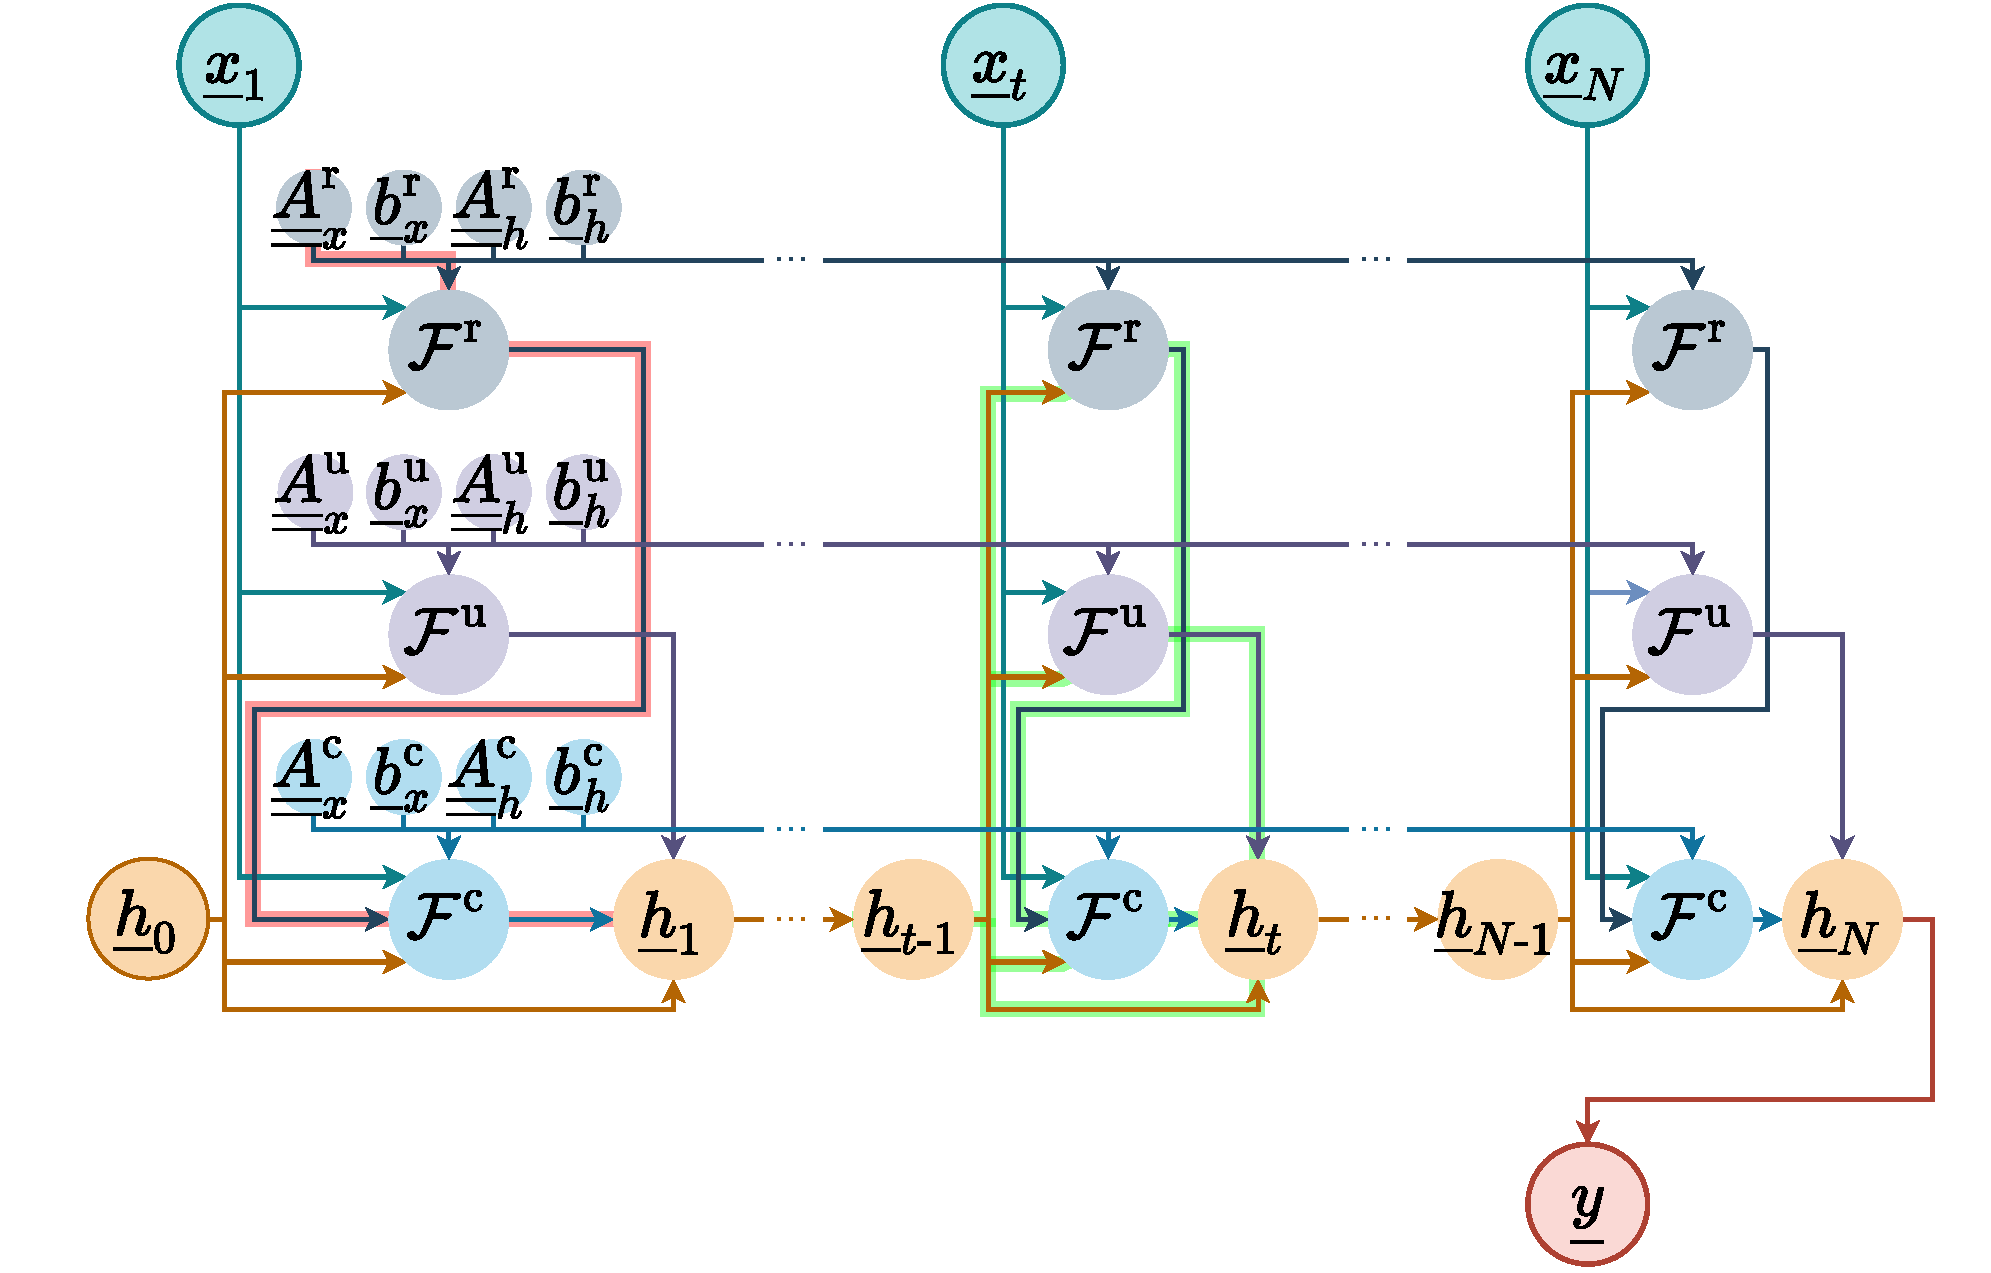
\includegraphics[width=0.9\textwidth]{own/gru_unfolded_intra_inter_paths.drawio.pdf}
    \caption[
        Unfolded GRU in many-to-one mode
    ]{
        Time-unfolded computation graph of a GRU layer in many-to-one mode,
        which maps
        the input sequence $\left(x_t\right)_{t\in\{1,\dots N\}}$ 
        to the single output $\underline y$ equal to the
        hidden state $\underline h_N$ of the last processing step.
        $\mathcal{F}^\text{r}$,
        $\mathcal{F}^\text{u}$
        and $\mathcal{F}^\text{c}$
        (see equ. \ref{eq:gru_reset}, \ref{eq:gru_update} and \ref{eq:gru_candidate})
        are the maps to the
        reset gate, update gate and candidate state, respectively.
        The map 
        $\mathcal{F}^\text{h}$ 
        (see equ. \ref{eq:gru_layer_map_hidden})
        yields the hidden states 
        $\left(h_t\right)_{t\in\{1,\dots N\}}$,
        whereas $\underline h_0$ is initialized.
        The trainable objects
        $\underline{\underline{A}}^\square_\square, \underline{b}^\square_\square$
        of the GRU layer
        are shared across all unfolded time steps.
        The backpropagation path of the intra-gradient with respect to 
        $\underline{\underline{A}}^\text{r}_x$
        (see equ. \ref{eq:gru_grad_intra_hidden_2_Arx}) 
        is highlighted in red for $t=1$.
        The backpropagation path of the inter-gradient 
        (see equ. \ref{eq:gru_grad_inter}) 
        is highlighted in green
        for $t$.
        \label{fig:gru_unfolded}}
\end{figure}
The GRU layer forwards the batches of 
single outputs to the subsequent layer of the ANN.
After passing the output layer of the ANN, the loss
of the batch is computed by averaging the losses of the batch elements
\begin{equation} \label{eq:loss_of_batch}
    L\left(\underline y_1, \dots, \underline y_{N^\text{batch}}\right) 
    = 
    \frac{1}{N^\text{batch}}
    \sum_{i=1}^{N^\text{batch}} L_i \left(\underline y_i\right).
\end{equation}
Gradient-based methods update the trainable parameters 
of the ANN with the goal to minimize the batch loss. 
To do this, they compute the gradients of the batch loss 
with respect to the trainable parameters. 
The update of the trainable parameters of the integrated GRU layer 
complies with
\begin{equation}
    \underset{\Theta}{\mathrm{argmin}}\ 
    L\left(\underline y_1, \dots, \underline y_{N^\text{batch}}\right).
\end{equation}
In conformity with Li \cite{li2016tutorial}, 
BPTT calculates the gradient of the batch loss 
with respect to an element $\theta \in \Theta$ 
in the set of trainable objects (see equ. \ref{eq:gru_params})
\begin{align} \label{eq:gru_grad_loss_2_theta}
    &\frac{\partial}{\partial \theta}
        L\left(\underline y_1, \dots, \underline y_{N^\text{batch}}\right)
    \nonumber \\ & \quad \overset{\textcolor{black}{(1)}}{=}
    \frac{1}{N^\text{batch}}
    \sum_{i=1}^{N^\text{batch}} 
    \frac{\partial}{\partial \theta}
    L_i \left(\underline y_i\right)
    \nonumber \\ & \quad \overset{\textcolor{black}{(2)}}{=}
    \frac{1}{N^\text{batch}}
    \sum_{i=1}^{N^\text{batch}} \left(
        \frac{\partial L_i}{\partial \underline y_i}
        \frac{\partial \underline y_i}{\partial \theta}
    \right)
    \nonumber \\ & \quad \overset{\textcolor{black}{(3)}}{=}
    \frac{1}{N^\text{batch}}
    \sum_{i=1}^{N^\text{batch}} \left[
        \frac{\partial L_i}{\partial \underline y_i}
        \sum_{j=1}^{N^{seq}} \left(
            \frac{\partial  \underline y_i}{\partial \underline h_{j, i}}
            \widehat{ \frac{\partial \underline h_{j, i}}{\partial \theta}}
        \right)
    \right]
    \nonumber \\ & \quad \overset{\textcolor{black}{(4)}}{=}
    \frac{1}{N^\text{batch}}
    \sum_{i=1}^{N^\text{batch}} \left\{
        \frac{\partial L_i}{\partial \underline y_i}
        \sum_{j=1}^{N^{seq}} \left[
            \prod_{k=j+1}^{N^{seq}} \left(
                \frac{\partial \underline h_{k, i}}{\partial \underline h_{k-1, i}}
            \right)
            \widehat{ \frac{\partial \underline h_{j, i}}{\partial \theta}}
        \right]
    \right\}.
    \\[2ex]
        &\textcolor{black}{\text{\footnotesize (1) 
            Batch loss (equ. \ref{eq:loss_of_batch})}} \nonumber \\
        &\textcolor{black}{\text{\footnotesize (2) 
            Chain rule}} \nonumber \\
        &\textcolor{black}{\text{\footnotesize (3) 
            BPTT (gradient $\widehat{\square}$ considers previous hidden states constant)}} \nonumber \\
        &\textcolor{black}{\text{\footnotesize (4) 
            Many-to-one (equ. \ref{equ:gru_output_many_to_one});
            chain rule applied to $\partial \underline y_i / \partial \underline h_{j, i}$}} \nonumber
\end{align}
In the above formula,
the gradient
$\widehat{\partial \underline h_{j, i} / \partial \theta}$
(hereinafter referred to as intra-gradient) 
treats all previous hidden states 
$\underline h_{\tilde j,\dots, i}, \ \tilde j \in \{0, j-1\}$ as constants.
In doing so, the intra-gradient covers the backpropagation path 
from the hidden state 
$\underline h_{j, i}$
to the trainable object 
$\theta$
only within the same time step $j$.
The full gradient covering all backpropagation paths to 
$\theta$, 
connects all intra-backpropagation paths through time to the output 
$\underline y _i$ 
by multiplying the intra-gradients with the corresponding chains 
of time step inter-gradients
$\partial \underline h_{k, i}/\partial \underline h_{k-1, i}$.



The following exemplarily derives the intra-gradient with respect to
$\theta=\underline{\underline{A}}^\text{r}_x$ 
(see fig \ref{fig:gru_unfolded} for the corresponding backpropagation path):
\begin{align} \label{eq:gru_grad_intra_hidden_2_Arx}
    \widehat{\frac{\partial \underline h_{t, i}}{\partial \underline{\underline{A}}^\text{r}_x}}
    &\overset{\textcolor{black}{(1)}}{=}
    \widehat{\frac{\partial}{\partial \underline{\underline{A}}^\text{r}_x}} \left\{
        \left[
            \underline 1 
            -
            \mathcal{F}^\text{u}\left(\chi\right)
        \right]
        \odot
        \mathcal{F}^\text{c} \left(\chi\right)
        +
        \mathcal{F}^\text{u}\left(\chi\right)
        \odot
        \underline h_{t\text -1,i}
    \right\}
    %\nonumber \\ & \quad \overset{\textcolor{black}{(2)}}{=}
    \nonumber \\ &\overset{\textcolor{black}{(2)}}{=}
    \mathrm{diag} \left[
        \underline 1 
        -
        \mathcal{F}^\text{u}\left(\chi\right)
    \right]
    \widehat{
        \frac{\partial \mathcal{F}^\text{c} \left(\chi\right)}
            {\partial \underline{\underline{A}}^\text{r}_x} 
    }
    \\[2ex]
    &\textcolor{black}{\text{\footnotesize (1) 
            Map to hidden state (equ. \ref{eq:gru_layer_current_hidden}, \ref{eq:gru_layer_map_hidden}); 
            $\chi :=  \left(\underline x_{t, i}, \underline h_{t\text{-}1, i}\right)$}} \nonumber \\
    &\textcolor{black}{\text{\footnotesize (2) 
        Sum rule;
    }} \nonumber \\
    &\textcolor{black}{\text{\footnotesize \qquad
        Map to update gate (equ. \ref{eq:gru_update}): 
        $\widehat{\partial \mathcal{F}^\text{u} / \partial \underline{\underline{A}}^\text{r}_x} = 0$ 
    }} \nonumber \\
    &\textcolor{black}{\text{\footnotesize \qquad
        Consider
        $\widehat{\partial \underline h_{t\text -1, i} / \partial \underline{\underline{A}}^\text{r}_x} = 0$;
    }} \nonumber \\
    &\textcolor{black}{\text{\footnotesize \qquad
        Hadamard product of 2 vectors (equ. \ref{eq:hadamard_product_two_vectors})
    }} \nonumber
\end{align}
with
\begin{align} \label{eq:gru_grad_intra_candidate_2_Arx}
    \widehat{
        \frac{\partial \mathcal{F}^\text{c} \left(\chi\right)}
            {\partial \underline{\underline{A}}^\text{r}_x}
    }
    & \overset{\textcolor{black}{(1)}}{=}
    \widehat{
        \frac{\partial}{\partial \underline{\underline{A}}^\text{r}_x} 
    }
    \left\{
        \overset{\scriptscriptstyle \odot}{\tanh} \left[
            \underbrace{
            \underline{\underline A}^\text{c}_{x}
            \underline x_{t,i}
            +
            \underline b^\text{c}_{x}
            +
            \mathcal{F}^\text{r}\left(\underline x_{t, i}, \underline h_{t\text -1, i}\right)
            \odot
            \left(
                \underline{\underline A}^\text{c}_{h}
                \underline h_{t\text -1,i}
                +
                \underline b^\text{c}_{h}
            \right)}_{:=\chi^\text{c}}
        \right]
    \right\}
    \nonumber \\ & \overset{\textcolor{black}{(2)}}{=}
    \mathrm{diag} \left[
        \frac{\partial}{\partial \chi^\text{c}}
        \overset{\scriptscriptstyle \odot}{\tanh} \left(\chi^\text{c}\right)
    \right] 
    \cdot 
    \widehat{
        \frac{\partial \chi^\text{c}}
            {\partial \underline{\underline{A}}^\text{r}_x} 
    }
    \nonumber \\ & \overset{\textcolor{black}{(3)}}{=}
    \mathrm{diag} \left[
        1 - \overset{\scriptscriptstyle \odot}{\tanh}{}^2 \left(\chi^\text{c}\right)
    \right] 
    \cdot
    \mathrm{diag} \left(
        \underline{\underline A}^\text{c}_{h}
        \underline h_{t-1,i}
        +
        \underline b^\text{c}_{h}
    \right)
    \widehat{
        \frac{\partial \mathcal{F}^\text{r}\left(\underline x_{t, i}, \underline h_{t\text -1, i}\right)}
            {\partial \underline{\underline{A}}^\text{r}_x} 
    }
    \\[2ex]
    &\textcolor{black}{\text{\footnotesize (1) 
            Map to candidate state (equ. \ref{eq:gru_candidate}); 
            $\chi :=  \left(\underline x_{t, i}, \underline h_{t\text{-}1, i}\right)$}} \nonumber \\
    &\textcolor{black}{\text{\footnotesize (2) 
        Chain rule;  
    }} \nonumber \\
    &\textcolor{black}{\text{\footnotesize \qquad
        Derivative of element-wise function
        (equ. \ref{eq:derivative_vector_elementwise_applied_function})
    }} \nonumber \\
    &\textcolor{black}{\text{\footnotesize (3) 
        Derivative of tanh (equ. \ref{eq:derivative_tanh}); 
    }} \nonumber \\
    &\textcolor{black}{\text{\footnotesize \qquad
    Hadamard product of 2 vectors (equ. \ref{eq:hadamard_product_two_vectors})
    }} \nonumber
\end{align}
and
\begin{align} \label{eq:gru_grad_intra_reset_2_Arx} 
    \widehat{
        \frac{\partial \mathcal{F}^\text{r}\left(\underline x_{t, i}, \underline h_{t\text -1, i}\right)}
            {\partial \underline{\underline{A}}^\text{r}_x} 
    }
    &\overset{\textcolor{black}{(1)}}{=}
    \widehat{
        \frac{\partial}{\partial \underline{\underline{A}}^\text{r}_x} 
    }
    \left[
        \overset{\scriptscriptstyle \odot}{\sigma} \left(
            \underbrace{
            \underline{\underline A}^\text{r}_{x}
            \underline x_{t,i}
            +
            \underline b^\text{r}_{x}
            +
            \underline{\underline A}^\text{r}_{h}
            \underline h_{t\text -1,i}
            +
            \underline b^\text{r}_{h}}_{:=\chi^\text{r}}
        \right)
    \right]
    \nonumber \\ & \overset{\textcolor{black}{(2)}}{=}
    \mathrm{diag} \left[
        \frac{\partial}{\partial \chi^\text{r}}
        \overset{\scriptscriptstyle \odot}{\sigma} \left(\chi^\text{r}\right)
    \right]
    \cdot
    \widehat{
        \frac{\partial \chi^\text{u}{}}
            {\partial \underline{\underline{A}}^\text{r}_x} 
    }
    \nonumber \\ & \overset{\textcolor{black}{(3)}}{=}
    \mathrm{diag} \left\{
        \overset{\scriptscriptstyle \odot}{\sigma} \left(\chi^\text{r}\right)
        \odot
        \left[
            1 -  \overset{\scriptscriptstyle \odot}{\sigma} \left(\chi^\text{r}\right)
        \right]
    \right\}
    \cdot
    \frac{\partial \underline{\underline A}^\text{r}_{x}\underline x_{t,i}}
        {\partial \underline{\underline{A}}^\text{r}_x} 
        .
    \\[2ex]
        &\textcolor{black}{\text{\footnotesize (1) 
            Map to reset gate (equ. \ref{eq:gru_reset})}} \nonumber \\
        &\textcolor{black}{\text{\footnotesize (2) 
            Chain rule;
        }} \nonumber \\
        &\textcolor{black}{\text{\footnotesize \qquad
            Derivative of element-wise function
            (equ. \ref{eq:derivative_vector_elementwise_applied_function})
        }} \nonumber \\
        &\textcolor{black}{\text{\footnotesize (3) 
            Derivative of sigmoid (equ. \ref{eq:derivative_sigmoid})
        }} \nonumber
\end{align}
For the calculation of the gradient
$\partial \left(\underline{\underline A}^\text{r}_{x}\underline x_{t,i}\right)
        /\partial \underline{\underline{A}}^\text{r}_x
$,
which is a three-dimensional tensor 
of only two-dimensional information content, 
refer to \cite{LearnedMiller}, for example.

As required by equation \ref{eq:gru_grad_loss_2_theta}, 
the following derives the inter-gradient
(see fig \ref{fig:gru_unfolded} for the corresponding backpropagation path):
%$\underline h_{t, i} = 
%\mathcal{F}^\text{h} \left(\underline x_{t, i}, \underline h_{t\text{-}1, i}\right)$
%and 
%$\chi :=  \left(\underline x_{t, i}, \underline h_{t\text{-}1, i}\right)$:
\begin{align} \label{eq:gru_grad_inter}
    \frac{\partial \underline h_{t, i}}{\partial \underline h_{t\text{-}1, i}}
    %\nonumber \\ & \quad \overset{\textcolor{black}{(1)}}{=}
    %\frac{\partial}{\partial \underline h_{t\text{-}1, i}}
    %\mathcal{F}^\text{h} \left(\underline x_{t, i}, \underline h_{t\text{-}1, i}\right)
    %\nonumber \\ & \quad \overset{\textcolor{black}{(1)}}{=}
    &\overset{\textcolor{black}{(1)}}{=}
    \frac{\partial}{\partial \underline h_{t\text{-}1, i}} \left\{
        \left[
            \underline 1 
            -
            \mathcal{F}^\text{u}\left(\chi\right)
        \right]
        \odot
        \mathcal{F}^\text{c} \left(\chi\right)
        +
        \mathcal{F}^\text{u}\left(\chi\right)
        \odot
        \underline h_{t\text -1,i}
    \right\}
    %\nonumber \\ & \quad \overset{\textcolor{black}{(2)}}{=}
    \nonumber \\ &\overset{\textcolor{black}{(2)}}{=}
    \frac{\partial}{\partial \underline h_{t\text{-}1, i}} \left\{
        \left[
            \underline 1 
            -
            \mathcal{F}^\text{u}\left(\chi\right)
        \right]
        \odot
        \mathcal{F}^\text{c} \left(\chi\right)
    \right\}
    +
    \frac{\partial}{\partial \underline h_{t\text{-}1, i}} \left\{
        \mathcal{F}^\text{u}\left(\chi\right)
        \odot
        \underline h_{t-1,i}
    \right\}
    %\nonumber \\ & \quad \overset{\textcolor{black}{(3)}}{=}
    \nonumber \\ & \overset{\textcolor{black}{(3)}}{=}
    - \mathrm{diag}\left[\mathcal{F}^\text{c} \left(\chi\right)\right] 
    \frac{\partial \mathcal{F}^\text{u}\left(\chi\right)}
        {\partial \underline h_{t\text{-}1, i}}
    +
    \mathrm{diag} \left[
        \underline 1 
        -
        \mathcal{F}^\text{u}\left(\chi\right)
    \right]
    \frac{\partial \mathcal{F}^\text{c} \left(\chi\right)}
        {\partial \underline h_{t\text{-}1, i}}
    \nonumber \\ &\qquad +
    \mathrm{diag} \left(\underline h_{t-1,i}\right)
    \frac{\partial \mathcal{F}^\text{u}\left(\chi\right)}
        {\partial \underline h_{t\text{-}1, i}}
    +
    \mathrm{diag} \left[
        \mathcal{F}^\text{u}\left(\chi\right)
    \right].
    \\[2ex]
    &\textcolor{black}{\text{\footnotesize (1) 
            Map to hidden state (equ. \ref{eq:gru_layer_current_hidden}, \ref{eq:gru_layer_map_hidden}); 
            $\chi :=  \left(\underline x_{t, i}, \underline h_{t\text{-}1, i}\right)$}} \nonumber \\
    &\textcolor{black}{\text{\footnotesize (2) 
        Sum rule
    }} \nonumber \\
    &\textcolor{black}{\text{\footnotesize (3) 
        Differentiation of Hadamard product of 2 vectors 
        (equ. \ref{eq:differentiation_hadamard_product_two_vectors})
    }} \nonumber
\end{align}
with
\begin{align} \label{eq:gru_grad_update_2_previous_hidden} 
    \frac{\partial
    \mathcal{F}^\text{u} \left(\underline x_{t, i}, \underline h_{t\text{-}1, i}\right)
    }{\partial \underline h_{t\text{-}1, i}}
    &\overset{\textcolor{black}{(1)}}{=}
    \frac{\partial}{\partial \underline h_{t\text{-}1, i}}
    \left[
        \overset{\scriptscriptstyle \odot}{\sigma} \left(
            \underbrace{
            \underline{\underline A}^\text{u}_{x}
            \underline x_{t,i}
            +
            \underline b^\text{u}_{x}
            +
            \underline{\underline A}^\text{u}_{h}
            \underline h_{t\text -1,i}
            +
            \underline b^\text{u}_{h}}_{:=\chi^\text{u}}
        \right)
    \right]
    \nonumber \\ & \overset{\textcolor{black}{(2)}}{=}
    \mathrm{diag} \left[
        \frac{\partial}{\partial \chi^\text{u}}
        \overset{\scriptscriptstyle \odot}{\sigma} \left(\chi^\text{u}\right)
    \right]
    \cdot \frac{\partial}{\partial \underline h_{t\text{-}1, i}} \chi^\text{u}{}
    \nonumber \\ & \overset{\textcolor{black}{(3)}}{=}
    \mathrm{diag} \left\{
        \overset{\scriptscriptstyle \odot}{\sigma} \left(\chi^\text{u}\right)
        \odot
        \left[
            1 -  \overset{\scriptscriptstyle \odot}{\sigma} \left(\chi^\text{u}\right)
        \right]
    \right\}
    \cdot \underline{\underline A}^\text{u}_{h},
    \\[2ex]
        &\textcolor{black}{\text{\footnotesize (1) 
            Map to update gate (equ. \ref{eq:gru_update})}} \nonumber \\
        &\textcolor{black}{\text{\footnotesize (2) 
            Chain rule;
        }} \nonumber \\
        &\textcolor{black}{\text{\footnotesize \qquad
            Derivative of element-wise function
            (equ. \ref{eq:derivative_vector_elementwise_applied_function})
        }} \nonumber \\
        &\textcolor{black}{\text{\footnotesize (3) 
            Derivative of sigmoid (equ. \ref{eq:derivative_sigmoid})
        }} \nonumber
\end{align}
and
\begin{align} \label{eq:gru_grad_candidate_2_previous_hidden}
    &\frac{\partial}{\partial \underline h_{t\text{-}1, i}}
    \mathcal{F}^\text{c}\left(\underline x_{t, i}, \underline h_{t\text -1, i}\right)
    \nonumber \\ & \quad \overset{\textcolor{black}{(1)}}{=}
    \frac{\partial}{\partial \underline h_{t\text{-}1, i}}
    \left\{
        \overset{\scriptscriptstyle \odot}{\tanh} \left[
            \underbrace{
            \underline{\underline A}^\text{c}_{x}
            \underline x_{t,i}
            +
            \underline b^\text{c}_{x}
            +
            \mathcal{F}^\text{r}\left(\underline x_{t, i}, \underline h_{t\text -1, i}\right)
            \odot
            \left(
                \underline{\underline A}^\text{c}_{h}
                \underline h_{t\text -1,i}
                +
                \underline b^\text{c}_{h}
            \right)}_{:=\chi^\text{c}}
        \right]
    \right\}
    \nonumber \\ & \quad \overset{\textcolor{black}{(2)}}{=}
    \mathrm{diag} \left[
        \frac{\partial}{\partial \chi^\text{c}}
        \overset{\scriptscriptstyle \odot}{\tanh} \left(\chi^\text{c}\right)
    \right] 
    \cdot 
    \frac{\partial}{\partial \underline h_{t\text{-}1, i}} \chi^\text{c}
    \nonumber \\ & \quad \overset{\textcolor{black}{(3)}}{=}
    \mathrm{diag} \left[
        1 - \overset{\scriptscriptstyle \odot}{\tanh}{}^2 \left(\chi^\text{c}\right)
    \right] 
    \nonumber \\ &\quad \quad  \cdot
    \left\{
        \mathrm{diag} \left(
            \underline{\underline A}^\text{c}_{h}
            \underline h_{t-1,i}
            +
            \underline b^\text{c}_{h}
        \right)
        \frac{\partial \mathcal{F}^\text{r}\left(\underline x_{t, i}, \underline h_{t\text -1, i}\right)}
        {\partial \underline h_{t\text -1, i}}
        +
        \mathrm{diag}\left[
            \mathcal{F}^\text{r}\left(\underline x_{t, i}, \underline h_{t\text -1, i}\right)
        \right]
        \underline{\underline A}^\text{c}_{h}
    \right\}.
    \\[2ex]
        &\textcolor{black}{\text{\footnotesize (1)
            Map to candidate state (equ. \ref{eq:gru_candidate})
        }} \nonumber \\
        &\textcolor{black}{\text{\footnotesize (2) 
            Chain rule of differentiation;  
        }} \nonumber \\
        &\textcolor{black}{\text{\footnotesize \qquad 
            Derivative of function applied element-wise on vector
            (equ. \ref{eq:derivative_vector_elementwise_applied_function})
        }} \nonumber \\
        &\textcolor{black}{\text{\footnotesize (3) 
            Derivative of hyperbolic tangent (equ. \ref{eq:derivative_tanh}); 
        }} \nonumber \\
        &\textcolor{black}{\text{\footnotesize \qquad
            Differentiation of Hadamard product of 2 vectors 
            (equ. \ref{eq:differentiation_hadamard_product_two_vectors})
        }} \nonumber
\end{align}
as well as (same structure as in equ. \ref{eq:gru_grad_update_2_previous_hidden})
%The in equation \ref{eq:gru_grad_candidate_2_previous_hidden} 
%required gradient of the current reset gate
%with respect to the previous hidden state shares the same structure
%with the gradient of equation \ref{eq:gru_grad_update_2_previous_hidden} 
%and is hence derived as
\begin{align}
    \frac{\partial}{\partial \underline h_{t\text{-}1, i}}
    \mathcal{F}^\text{r} \left(\underline x_{t, i}, \underline h_{t\text{-}1, i}\right)
    &=
    \mathrm{diag} \left\{
        \overset{\scriptscriptstyle \odot}{\sigma} \left(\chi^\text{r}\right)
        \odot
        \left[
            1 -  \overset{\scriptscriptstyle \odot}{\sigma} \left(\chi^\text{r}\right)
        \right]
    \right\}
    \cdot \underline{\underline A}^\text{r}_{h}
    \nonumber \\
    \text{with } \chi^\text{r} & :=
    \underline{\underline A}^\text{r}_{x}
            \underline x_{t,i}
            +
            \underline b^\text{r}_{x}
            +
            \underline{\underline A}^\text{r}_{h}
            \underline h_{t\text -1,i}
            +
            \underline b^\text{r}_{h}.
\end{align}
The above derivations revert to the following equations.
Equations (4.5.73) and (4.5.17) of Abramowitz and Stegun \cite{D.1966}
yield the derivative of the hyperbolic tangent as
\begin{equation} \label{eq:derivative_tanh}
    \frac{\text d}{\text d x} \tanh (x) = 1 - \tanh^2 (x).
\end{equation}
The derivative of the sigmoid function (e.g., \cite{Minai1993}) is
\begin{equation} \label{eq:derivative_sigmoid}
    \frac{\text d}{\text d x} \sigma \left(x\right) 
    = 
    \sigma \left(x\right) 
    \left[
        1 - \sigma \left(x\right)
    \right].
\end{equation}
The Hadamard product of two vectors \cite{Brookes2020} equates to the 
matrix product of a diagonal matrix and a vector 
\begin{equation} \label{eq:hadamard_product_two_vectors}
    \underline x_1 \odot \underline x_2 
= 
    \mathrm{diag} \left(\underline x_1\right) \underline x_2 
=   
    \mathrm{diag} \left(\underline x_2\right) \underline x_1.
\end{equation}
Applying the product rule of differentiation 
yields the derivative of the Hadamard product of two vectors
\begin{equation} \label{eq:differentiation_hadamard_product_two_vectors}
    \frac{\partial}{\partial t} \left(
        \underline x_1 \odot \underline x_2 
    \right)
    =   
    \mathrm{diag} \left(\underline x_2\right)
    \frac{\partial \underline x_1}{\partial t} 
    +
    \mathrm{diag} \left(\underline x_1\right)
    \frac{\partial \underline x_2}{\partial t}.
\end{equation}
The derivative of a function
$f:\mathbb{R}\rightarrow\mathbb{R}$ applied element-wise to a vector $\underline x$
is the diagonal matrix built from the derivative of the function applied element-wise on the vector
\begin{equation} \label{eq:derivative_vector_elementwise_applied_function}
        \frac{\partial}{\partial \underline x} 
        \overset{\scriptscriptstyle \odot}{f} \left(
                \underline x
            \right)
    =
        \mathrm{diag} \left[
            \overset{\scriptscriptstyle \odot}{f'}  \left(
                \underline x
            \right)
        \right].
\end{equation}
The calculation of the differential of the function yields the above statement
\begin{align}
    &\frac{\text d}{\text d \underline x}
    \overset{\scriptscriptstyle \odot}{f} \left(
        \underline x
    \right)
    \cdot \text d \underline x
\overset{\textcolor{black}{(1)}}{=}
    \text d 
    \overset{\scriptscriptstyle \odot}{f} \left(
        \underline x
    \right)
\overset{\textcolor{black}{(2)}}{=}
    \left[
        \overset{\scriptscriptstyle \odot}{f'}  \left(
            \underline x
        \right)
    \right]
    \odot \text d \underline x
\overset{\textcolor{black}{(3)}}{=}
    \mathrm{diag} \left[
        \overset{\scriptscriptstyle \odot}{f'}  \left(
            \underline x
        \right)
    \right]\cdot
    \text d \underline x.
    \\[2ex]
        &\quad\textcolor{black}{\text{\footnotesize (1) Relation of differential and derivative}} \nonumber \\
        &\quad\textcolor{black}{\text{\footnotesize (2) Chain rule element-wise applied}} \nonumber \\
        &\quad\textcolor{black}{\text{\footnotesize (3) Hadamard product of 2 vectors (equ. \ref{eq:hadamard_product_two_vectors})}}
\end{align}
\chapter{Autonomous Navigation Method}
\label{mainone}
\textit{
DELETEME: In this chapter you start addressing your actual problem. Therefore, it makes often sense to make a detailed problem analysis first (if not done in introduction). You should be sure about what to do and how. As writtin in the background part, it might also make sense to include complex background information or papers you are basing on in this analysis. If you are solving a software problem, you should follow the state of the art of software development which basically includes: problem analysis, design, implementation, testing, and deployment. Maintenance is often also described but I believe this will not be required for most theses. Code should be placed in the appendix unless it is solving an essential aspect of your work.
}





In order to investigate the effect of temporal comprehension in machine-learning-based, autonomous navigation of drones,
this master thesis extends the navigation method of Kaufmann, Loquercio et. al [?] is minimally adjusted and extended with a recurrent convolutional neural network.
This chapter \dots



\section{Reference systems}
In this thesis, the coordinates of a point 
$\pos[]{}{}{}{}$
relate to either the global, the local or the image reference system
\begin{equation}
    \pos[]{}{}{\grs}{} = \begin{bmatrix}
        \x[]{}{}{\grs}{} \\ \y[]{}{}{\grs}{} \\ \z[]{}{}{\grs}{}
    \end{bmatrix} \in \mathbb{R}^3
    ,\quad 
    \pos[]{}{}{\lrs}{} = \begin{bmatrix}
        \x[]{}{}{\lrs}{} \\ \y[]{}{}{\lrs}{} \\ \z[]{}{}{\lrs}{}
    \end{bmatrix} \in \mathbb{R}^3
    ,\quad 
    \pos[]{}{}{\irs}{} = \begin{bmatrix}
        \x[]{}{}{\irs}{} \\ \y[]{}{}{\irs}{}
    \end{bmatrix} \in \left[\text -1, 1\right]^2.
\end{equation}


The 3D global reference system
is fixed to an arbitrary point on earth
and is hence quasi inertial.
It is spanned by the orthonormal basis
which, related to the global reference system,
equates to the standard basis of $\mathbb{R}^3$
\begin{equation}
    \left\{
        \unitvec[]{\text G}{x}{}{},
        \unitvec[]{\text G}{y}{}{},
        \unitvec[]{\text G}{z}{}{}
    \right\}
    \quad \text{with} \quad 
    \unitvec[]{\text G}{x}{\grs}{} = \begin{bmatrix} 1 \\ 0 \\ 0 \end{bmatrix},\ 
    \unitvec[]{\text G}{y}{\grs}{} = \begin{bmatrix} 0 \\ 1 \\ 0 \end{bmatrix},\ 
    \unitvec[]{\text G}{z}{\grs}{} = \begin{bmatrix} 0 \\ 0 \\ 1 \end{bmatrix}.
\end{equation}


The local reference system (see figure \ref{fig:local_reference_system}) is fixed to the moving drone.
It is spanned by the orthonormal basis,
whose origin is located at the optical center of the drone's onboard camera,
\begin{equation}
    \left\{
        \unitvec[]{\text L}{x}{}{},
        \unitvec[]{\text L}{y}{}{},
        \unitvec[]{\text L}{z}{}{}
    \right\}
    \quad \text{with} \quad 
    \unitvec[]{\text L}{x}{\lrs}{} = \begin{bmatrix} 1 \\ 0 \\ 0 \end{bmatrix},\ 
    \unitvec[]{\text L}{y}{\lrs}{} = \begin{bmatrix} 0 \\ 1 \\ 0 \end{bmatrix},\ 
    \unitvec[]{\text L}{z}{\lrs}{} = \begin{bmatrix} 0 \\ 0 \\ 1 \end{bmatrix}.
\end{equation}
The unit vector 
$\unitvec[]{\text L}{x}{}{}$ 
points along the optical axis of the camera
in the flight direction of the drone.
The unit vector
$\unitvec[]{\text L}{z}{}{}$ 
points in the direction of the forces generated by the drone's rotors
and is parallel to the vertical axis of the image plane of the drone's onboard camera.
The unit vector 
$\unitvec[]{\text L}{y}{}{}$ 
points to the left of the drone
and parallels the horizontal axis of the image plane.






The image reference system (see figure \ref{fig:image_reference_system}) 
is superimposed on the images of the drone's onboard camera.
This 2-dimensional system is spanned by the orthonormal basis
\begin{equation}
    \left\{
        \unitvec[]{\text I}{x}{}{},
        \unitvec[]{\text I}{y}{}{}
    \right\}
    \quad \text{with} \quad 
    \unitvec[]{\text I}{x}{\irs}{} = \begin{bmatrix} 1 \\ 0 \end{bmatrix},\ 
    \unitvec[]{\text I}{y}{\irs}{} = \begin{bmatrix} 0 \\ 1 \end{bmatrix}.
\end{equation}
The origin of the image reference system 
is located at the center of the image plane.
The unit vector 
$\unitvec[]{\text I}{x}{}{}$  
points rightwards along the vertical axis of the image plane.
The unit vector 
$\unitvec[]{\text I}{y}{}{}$  
points upwards along the horizontal axis of the image plane.
A point on the image plane 
is bounded by the left and right
$ -1 \le \x[]{}{}{\irs}{} \le 1 $
as well as the lower and upper
$ -1 \le \y[]{}{}{\irs}{} \le 1 $
border of the image plane.
%The global reference system 
%is only referred to 
%by the expert system (see section)
%which makes navigation decisions based on globally consistent information
%when generating training data for the ANN module.
%The autonomous navigation method, 
%with the fully trained ANN module making the navigation decisions,
%exclusively resorts to data from onboard sensors,
%which is relative to the drone and its onboard camera.
%The method, therefore, operates only within the local and image reference system.
\begin{figure}[h]
    \centering
    \subfloat[
        Local reference system
    ]{
        \label{fig:local_reference_system}
        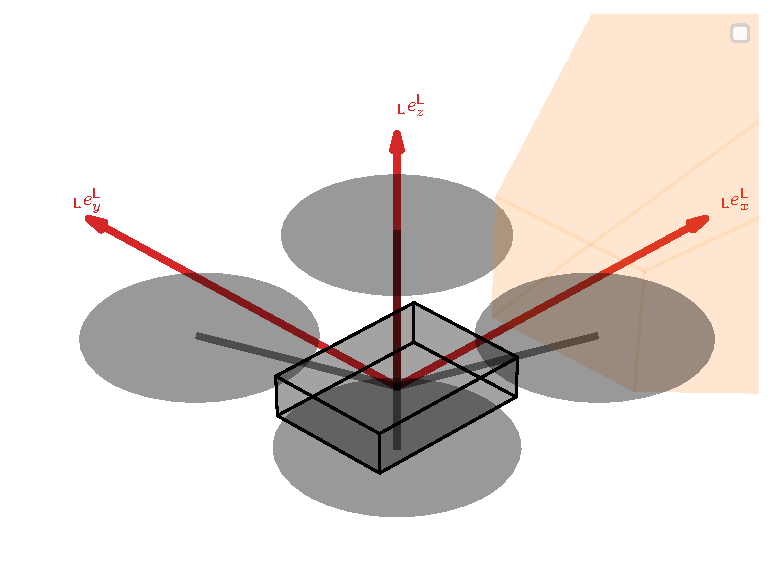
\includegraphics[width=0.441\textwidth]{own/local_reference_system.pdf}
    }                
    \subfloat[
        Image reference system
    ]{
        \label{fig:image_reference_system}
        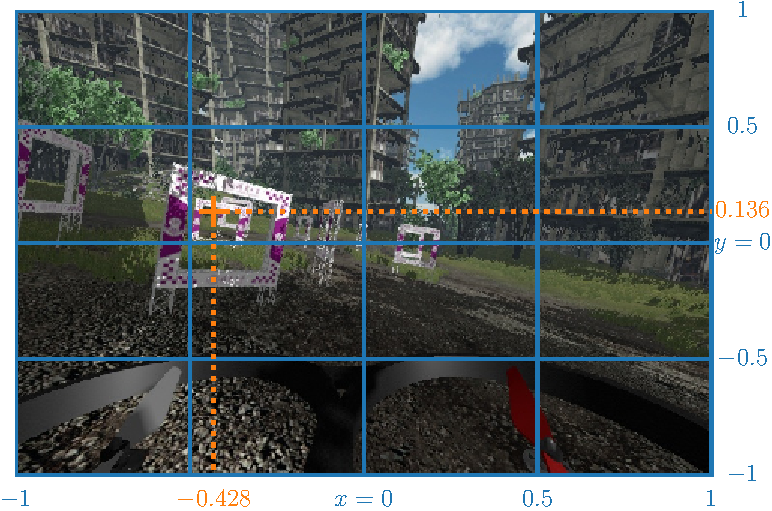
\includegraphics[width=0.5\textwidth]{own/image_reference_system.pdf}
    }
    \caption[
        The local and the image reference system
    ]{
        The local and the image reference system. 
        The local reference system (red) is aligned with the drone's onboard camera. 
        The image reference system (blue) is superimposed on the images from the onboard camera.
        The pictured, exemplary waypoint
        $\pos[]{\wayp}{}{\irs}{} = \begin{bmatrix} -0.428 & 0.136 \end{bmatrix}^T$
        (orange) with respect to the image reference system
        is part of the label for the underlying image.
        \label{fig:local_and_image_reference_system}
    }
\end{figure}
%https://www.researchgate.net/figure/Pin-hole-camera-model-terminology-The-optical-center-pinhole-is-placed-at-the-origin_fig10_317498100





\paragraph*{Transformation between the global and the local reference system} $\ $\\
The drone's position
$\pos[]{\drone}{}{\grs}{}$
and quaternion orientation
$\quat[]{\drone}{}{\grs}{}$
with respect to the global reference system
are the parameters that determine the bidirectional transformation
between the global and the local reference system.
The following bases on quaternion mathematics,
for which one can consult, e.g., \cite{Parent}.
A point given in the coordinates of the global reference system
can be expressed in the coordinates of the local reference system
with the transformation
\begin{align} \label{equ:global_to_local_transformation}
    \trafo[]{}{\lrs\grs}{}{}
    :\ 
    \mathbb{R}^3 \rightarrow \mathbb{R}^3
    ; \quad
    \pos[]{}{}{\grs}{} \mapsto \pos[]{}{}{\lrs}{}
    =
    %\begin{cases}
        \mathcal{P} \left[
            \mathrm{inv} \left( \quat[]{\drone}{}{\grs}{} \right)
            *
            \mathcal{Q} \left( \pos[]{}{}{\grs}{} - \pos[]{\drone}{}{\grs}{} \right)
            *
            \quat[]{\drone}{}{\grs}{}
        \right], 
        %& \text{if } \quat[]{\drone}{}{\grs}{} \ne \underline 0 \\
        %\pos[]{}{}{\grs}{} - \pos[]{\drone}{}{\grs}{}, 
        %& \text{else}.
    %\end{cases}
\end{align}
Reversely, a point given in the coordinates of the local reference system
can be expressed in the coordinates of the global reference system
with the transformation
\begin{align} \label{eq:local_to_global_transformation}
    \trafo[]{}{\grs\lrs}{}{}
    :\ 
    \mathbb{R}^3 \rightarrow \mathbb{R}^3
    ; \quad
    \pos[]{}{}{\lrs}{} \mapsto \pos[]{}{}{\grs}{}
    =
    %\begin{cases}
        \mathcal{P} \left[
            \quat[]{\drone}{}{\grs}{}
            *
            \mathcal{Q} \left( \pos[]{}{}{\lrs}{} \right)
            *
            \mathrm{inv} \left( \quat[]{\drone}{}{\grs}{} \right)
        \right] + \pos[]{\drone}{}{\grs}{}, 
        %& \text{if } \quat[]{\drone}{}{\grs}{} \ne \underline 0 \\
        %\pos[]{}{}{\lrs}{} + \pos[]{\drone}{}{\grs}{}, 
        %& \text{else}.
    %\end{cases}
\end{align}
In the two above transformations,
the mapping $\mathcal{Q}$
of a point to its quaternion representation 
and the reverse mapping $\mathcal{P}$ 
of a quaternion representation to its point  
are given by
\begin{align}
    \mathcal{Q}
    :\ 
    & \mathbb{R}^3 \rightarrow \mathbb{R}^4
    ;\
    \pos[]{}{}{}{} = \begin{bmatrix} \x[]{}{}{}{} \\ \y[]{}{}{}{} \\ \z[]{}{}{}{} \end{bmatrix} 
    \mapsto
    \quat[]{}{}{}{} = \begin{bmatrix} w \\ \underline p \end{bmatrix} 
    \text{ with } w = 0
    \nonumber \\
    \mathcal{P}
    :\ 
    &\mathbb{R}^4 \rightarrow \mathbb{R}^3
    ;\
    \quat[]{}{}{}{} = \begin{bmatrix} w \\ \underline p \end{bmatrix} 
    \mapsto
    \pos[]{}{}{}{} = \begin{bmatrix} \x[]{}{}{}{} \\ \y[]{}{}{}{} \\ \z[]{}{}{}{} \end{bmatrix}.
\end{align}
Moreover, the operator $*$ denotes the multiplication of two quaternions which is given by
\begin{align}
    \quat[]{}{1}{}{} * \quat[]{}{2}{}{}
    = 
    \begin{bmatrix}
        w_1 w_2 - \pos[]{T}{1}{}{} \pos[]{}{2}{}{}\\ 
        w_1 \pos[]{}{2}{}{} + w_2 \pos[]{}{1}{}{} + \pos[]{}{1}{}{} \times \pos[]{}{2}{}{}
    \end{bmatrix}.
\end{align}
Finally, the inversion of a quaternion is given by
\begin{align}
    \mathrm{inv}(\quat[]{}{}{}{}) 
    = 
    \frac{1}{\| \quat[]{}{}{}{} \|_2}
    \begin{bmatrix} w \\ \text - \pos[]{}{}{}{} \end{bmatrix}.
\end{align}
The two above transformations are the inversion of each other.
Therefore, points can be transformed between the global and local reference system
without information loss
\begin{equation}
    \trafo[]{}{\grs\lrs}{}{} \circ \trafo[]{}{\lrs\grs}{}{} 
    \left( \pos[]{}{}{\grs}{} \right)
    =
    \pos[]{}{}{\grs}{}
    ,\quad
    \trafo[]{}{\lrs\grs}{}{} \circ \trafo[]{}{\grs\lrs}{}{} 
    \left( \pos[]{}{}{\lrs}{} \right)
    =
    \pos[]{}{}{\lrs}{}.
\end{equation}
In the above equations, the operator $\circ$ denotes the composition of two functions.



\paragraph*{Transformation between the local and the image reference system} $\ $\\
The horizontal
$\ang[\user]{\camera}{\text h}{}{}$
and the vertical
$\ang[\user]{\camera}{\text v}{}{}$
angle of view
of the drone's onboard camera
are the parameters 
that determine the bidirectional transformation 
between the local and the image reference system.
A point given in the coordinates of the local reference system
is expressed in the coordinates of the image reference system with the transformation
\begin{align} \label{equ:local_to_image_transformation}
    \trafo[]{}{\irs\lrs}{}{}
    :\ 
    \mathbb{R}^3 \rightarrow \left[ \text{-}1, 1 \right]^2
    ; \quad
    \pos[]{}{}{\lrs}{} \mapsto \pos[]{}{}{\irs}{}
    =
    \begin{bmatrix}
        \maxof{\text -1}{
            \minof{
                \frac{\text -2}{\ang[\user]{\camera}{\text h}{}{}}
                \mathrm{atan2}\left( \y[]{}{}{\lrs}{}, \x[]{}{}{\lrs}{} \right)
            }{1}
        }
        \\
        \maxof{\text -1}{
            \minof{
                \frac{2}{\ang[\user]{\camera}{\text v}{}{}}
            \mathrm{atan2} \left( \z[]{}{}{\lrs}{}, \| \pos[]{}{}{\lrs}{} \|_2 \right)
            }{1}
        }
    \end{bmatrix}
    .
\end{align}
The above transformation
can be interpreted as the projection of a point onto the image plane 
of the drone's onboard camera.
It can be devided into three steps.
First, the vector from the optical center of the camera 
to the point to be transformed
is mapped to its yaw
$\mathrm{atan2}\left( \y[]{}{}{\lrs}{}, \x[]{}{}{\lrs}{} \right)$
and pitch 
$\mathrm{atan2} \left( \z[]{}{}{\lrs}{}, \| \pos[]{}{}{\lrs}{} \|_2 \right)$
angle, both, with respect to the image reference system.
Second these angles are normalized by 
the half of the horizontal 
$\ang[\user]{\camera}{\text h}{}{}$ 
and the half of the vertical
$\ang[\user]{\camera}{\text v}{}{}$
angle of view of the camera, respectively.
Third, these normalized angles are bounded to be in the interval from minus to plus one.
This boundary takes into account 
that an artifical neural network, which inputs images, 
has no basis for predictions 
that relate to objects that are not within the camera's field of view.
As a projection from 3D to 2D, the above transformation is accompanied by information loss
and is hence not bijective.

A point given in the coordinates of the image reference system is expressed
in the coordinates of the local reference system with the reverse transformation
\begin{align} \label{eq:image_to_local_transformation}
    \trafo[]{}{\lrs\irs}{}{}
    &:\ 
    \mathbb{R}_{\ge 0}, \left[ \text{-}1, 1 \right]^2 \rightarrow \mathbb{R}^3
    ; \quad
    d, \pos[]{}{}{\irs}{} \mapsto \pos[]{}{}{\lrs}{}
    =
    d \begin{bmatrix}
        \cos \left( \ang[]{}{y}{\lrs}{} \right) \\
        \cos \left( \ang[]{}{y}{\lrs}{} \right) \\
        \sin \left( \ang[]{}{y}{\lrs}{} \right)
    \end{bmatrix} \odot \begin{bmatrix}
        \cos \left( \ang[]{}{z}{\lrs}{} \right) \\
        \sin \left( \ang[]{}{z}{\lrs}{} \right) \\
        1
    \end{bmatrix}
    \nonumber \\
    & \qquad \text{with} \quad
    \ang[]{}{z}{\lrs}{}
    = 
    \text - \frac{\ang[\user]{\camera}{\text h}{}{}}{2} \cdot \x[]{}{}{\irs}{}
    ,\quad 
    \ang[]{}{y}{\lrs}{}
    = 
    \frac{\ang[\user]{\camera}{\text v}{}{}}{2} \cdot \y[]{}{}{\irs}{}.
\end{align}
In the above transformation,
the operator 
$\odot$ 
denotes the Hadamard product, 
i.e., the element-wise product of two equally dimensioned matrices.
Because the 2D coordinates of the image reference system
can only contain information about the direction of a point,
the above transformation to 3D requires the additional input of a backprojection length $d$.

In contrast to the transformations 
$\trafo[]{}{\lrs\grs}{}{}$
and 
$\trafo[]{}{\grs\lrs}{}{}$
between the global and the local reference system,
the transformations 
$\trafo[]{}{\irs\lrs}{}{}$
and 
$\trafo[]{}{\lrs\irs}{}{}$
between the local and the image reference system
are not invertible.
However, for relevant points
located within the camera's field of view
and a well chosen backprojection length,
it is assumed that the transformations approximately invert each other
\begin{equation}
    \trafo[]{}{\lrs\irs}{}{} \left[
        d, \trafo[]{}{\irs\lrs}{}{} \left( \pos[]{}{}{\lrs}{} \right)
    \right]
    \approx
    \pos[]{}{}{\lrs}{}
    ,\quad
    \trafo[]{}{\irs\lrs}{}{}
    \circ 
    \trafo[]{}{\lrs\irs}{}{} \left(
        d, \pos[]{}{}{\irs}{}
    \right)
    \approx
    \pos[]{}{}{\irs}{}.
\end{equation}





\paragraph*{Transformation between the global and the image reference system} $\ $\\
The bidirectional transformations of points between the global and the image reference frame
are the compositions of the transformations via the intermittent local reference system
\begin{align} \label{eq:global_image_transformations}
    \trafo[]{}{\irs\grs}{}{}
    &=
    \trafo[]{}{\irs\lrs}{}{} \circ \trafo[]{}{\lrs\grs}{}{}
    :\ 
    \mathbb{R}^3 \rightarrow \left[\text{-} 1, 1\right]^2 
    \nonumber \\
    \trafo[]{}{\grs\irs}{}{}
    &=
    \trafo[]{}{\grs\lrs}{}{} \circ \trafo[]{}{\lrs\irs}{}{}
    :\ 
    \mathbb{R}_{\ge 0}, \left[\text{-} 1, 1\right]^2 \rightarrow \mathbb{R}^3.
\end{align}
Due to the fact that
$\trafo[]{}{\lrs\grs}{}{}$
and
$\trafo[]{}{\grs\lrs}{}{}$
are the inverse of each other
and the assumption that
$\trafo[]{}{\irs\lrs}{}{}$
and
$\trafo[]{}{\lrs\irs}{}{}$
approximately invert each other within a relevant range,
the above compositions are expected to also approximately invert each other within this relevant range
\begin{equation}
    \trafo[]{}{\grs\irs}{}{} \left[
        d, \trafo[]{}{\irs\grs}{}{} \left( \pos[]{}{}{\grs}{} \right)
    \right]
    \approx
    \pos[]{}{}{\grs}{}
    ,\quad
    \trafo[]{}{\irs\grs}{}{}
    \circ 
    \trafo[]{}{\grs\irs}{}{} \left(
        d, \pos[]{}{}{\irs}{}
    \right)
    \approx
    \pos[]{}{}{\irs}{}.
\end{equation}

%\begin{figure}
%    \centering
%    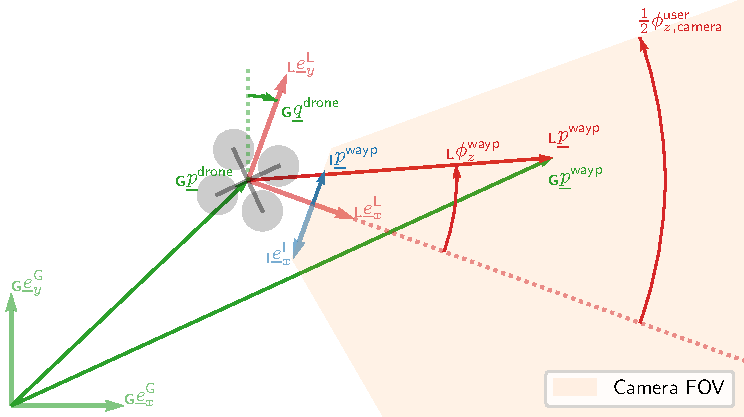
\includegraphics[width=0.9\textwidth]{own/global_via_local_to_image_transformation_2d.pdf}
%    \caption[
%        Schematic 2D depiction
%        of the transformation of the waypoint 
%        from the global via the local to the image reference system.
%    ]{
%        Schematic 2D depiction
%        of the transformation of the waypoint 
%        from the global ${}_\textbf{G}\square$ 
%        via the local ${}_\textbf{L}\square$ 
%        to the image ${}_\textbf{I}\square$ reference system.
%        Unit vectors 
%        $\underline e_\square \in \mathbb{R}^3,\ \left\|\underline e_\square \right\|_2 = 1$ 
%        spanning the individual reference systems,
%        points $\underline p^\square \in \mathbb{R}^3$,
%        quaternions $\underline q^\square \in \mathbb{R}^4$
%        and angles $\phi_\square^\square  \in \mathbb{R}$
%        relative to the global, local or image reference system
%        are colored in green, red or blue, respectively.
%        %Unit vectors are drawn
%        %with a greater linewidth and lower opacity 
%        %than the positions, quaternions and angles.
%        The z unit vectors 
%        ${}_\textbf{G} e^\text{G}_z$
%        and
%        $\ {}_\textbf{L} e^\text{L}_z$ 
%        of the global and local reference system,
%        the y unit vector 
%        ${}_\textbf{I} e^\text{I}_y$ 
%        of the image reference system
%        and the pitch angle 
%        $\phi^\text{user}_{y,\text{camera}}$
%        of view of the camera
%        are not pictured
%        in this 2D representation.
%        %but point in the direction of the reader.
%        The field of view (FOV) of the onboard camera of the drone
%        is marked with a low-opaque orange.
%
%        The global position
%        ${}_\textbf{G}\underline p^\text{drone}$
%        and quaternion orientation
%        ${}_\textbf{G}\underline q^\text{drone}$
%        of the drone,
%        the yaw
%        $\phi^\text{user}_{z,\text{camera}}$
%        and pitch
%        $\phi^\text{user}_{y,\text{camera}}$ 
%        angle of view of the camera
%        as well as the global position of the waypoint
%        ${}_\textbf{G}\underline p^\text{wayp}$
%        are known.
%        First, the local position of the waypoint
%        ${}_\textbf{L}\underline p^\text{wayp}$
%        is computed by applying the transformation
%        $T_\textbf{LG}$
%        (equation \ref{equ:global_to_local_transformation}).
%        Second, 
%        ${}_\textbf{L}\underline p^\text{wayp}$
%        is transformed with 
%        $T_\textbf{IL}$
%        (equation \ref{equ:local_to_image_transformation})
%        yielding 
%        the position of the waypoint
%        ${}_\textbf{I}\underline p^\text{wayp}$ 
%        with respect to the image reference system.
%        $T_\textbf{LG}$ is fully determined by 
%        ${}_\textbf{G}\underline p^\text{drone}$ 
%        and 
%        ${}_\textbf{G}\underline q^\text{drone}$.
%        $T_\textbf{IL}$ is fully determined by
%        $\phi^\text{user}_{z,\text{camera}}$
%        and
%        $\phi^\text{user}_{y,\text{camera}}$.
%        \label{fig:trafo}
%    }
%\end{figure}






%%%%%%%%%%%%%%%%%%%%%%%%%%%%%%%%%%%%%%%%%%%
\section{ANN module}\label{sec:ann_module}
%
%
\newcommand{\R}[1]{\mathbb{R}^{#1}}
\newcommand{\setR}[1]{\left[#1\right]}

\newcommand{\setOfAllPosInts}{\mathbb{N}_{>0}}
\newcommand{\setOfInts}[1]{\left\{ #1 \right\}}
\newcommand{\placeholder}{\square}
\newcommand{\floor}[1]{\left\lfloor #1 \right\rfloor}
\newcommand{\series}[1]{\left(#1\right)}
\newcommand{\tuple}[1]{\left(#1\right)}
%
\newcommand{\rawRGB}{\img[]{\camera}{}{}{}}
\newcommand{\rawRGBFullInt}{\num[]{\camera}{\mxm}{}{}}
\newcommand{\rawRGBHeight}{\num[]{\camera}{\height}{}{}}
\newcommand{\rawRGBWidth}{\num[]{\camera}{\widthh}{}{}}
\newcommand{\rawRGBTimeStep}{\dur[]{\camera}{}{}{}}
\newcommand{\preprocRGB}[1]{\img[]{\preprocessed}{#1}{}{}}
\newcommand{\IMULinAcc}{\acc[\hat]{\imu}{}{\lrs}{}}
\newcommand{\IMUAngVel}{\angvel[\hat]{\imu}{}{\lrs}{}}
\newcommand{\IMUTimeStep}{\dur[]{\imu}{}{}{}}
\newcommand{\optFeatVec}[1]{\featvec[]{\optional}{#1}{}{}}
\newcommand{\CNNMap}{\Func[\user]{\cnn}{}{}{}}
\newcommand{\CNNNumC}{\num[]{\cnn}{\channel}{}{}}
\newcommand{\CNNHeight}{\num[]{\cnn}{\height}{}{}}
\newcommand{\CNNWidth}{\num[]{\cnn}{\widthh}{}{}}
\newcommand{\CNNOutp}{\num[]{\cnn}{\outp}{}{}}
\newcommand{\visFeatVec}[1]{\featvec[]{\visual}{#1}{}{}}
\newcommand{\CNNNumP}{\num[]{\cnn}{\params}{}{}}
\newcommand{\CATMap}{\Func[]{\cat}{}{}{}}
\newcommand{\CATInp}[1]{\num[]{\cat}{#1}{}{}}
\newcommand{\CATNumP}{\num[]{\cat}{\params}{}{}}
%
\newcommand{\batchSize}{\num[\user]{\batch}{}{}{}}
\newcommand{\seqLen}{\num[\user]{\seq}{}{}{}}
\newcommand{\mainFreq}{\freq[\user]{\main}{}{}{}}
\newcommand{\resizeFact}{\anything[\user]{\cnn}{\text{resize}}{}{}{s}}
%
%
The ANN module performs the function of making navigation decisions
within the autonomous navigation method.
Figure \ref{fig:perception_and_reasoning} shows the 
information flow of this decision making process.
The ANN module infers its decisions exclusively 
on the basis of preprocessed data from sensors onboard the drone.
It comprises the five submodules named CNN, CAT, GRU, FC and HEAD.
This modular design enables a high flexibility for the experiments
with the different ANN module variants in chapter \ref{maintwo}.
All variants have in common that,
first, the order of the submodules is fixed
and, second, the outer submodules (CNN and HEAD)
are always activated.
The latter ensures the minimum functionality of the ANN module
of extracting visual features of the preprocessed 
RGB images from the drone's onboard camera
and mapping them to navigation decisions.
The variants can differ in that
the user specifies the design parameters of 
the (inner and outer) individual submodules.
This can include the deactivation (reduction to the identity map)
of the individual inner submodules (CAT, GRU and FC).
The inner submodules perform the functions of
inputting optional features (CAT),
extracting temporal features (GRU)
and increasing the general complexity of the ANN module (FC).

\begin{figure}[h]
    \centering
    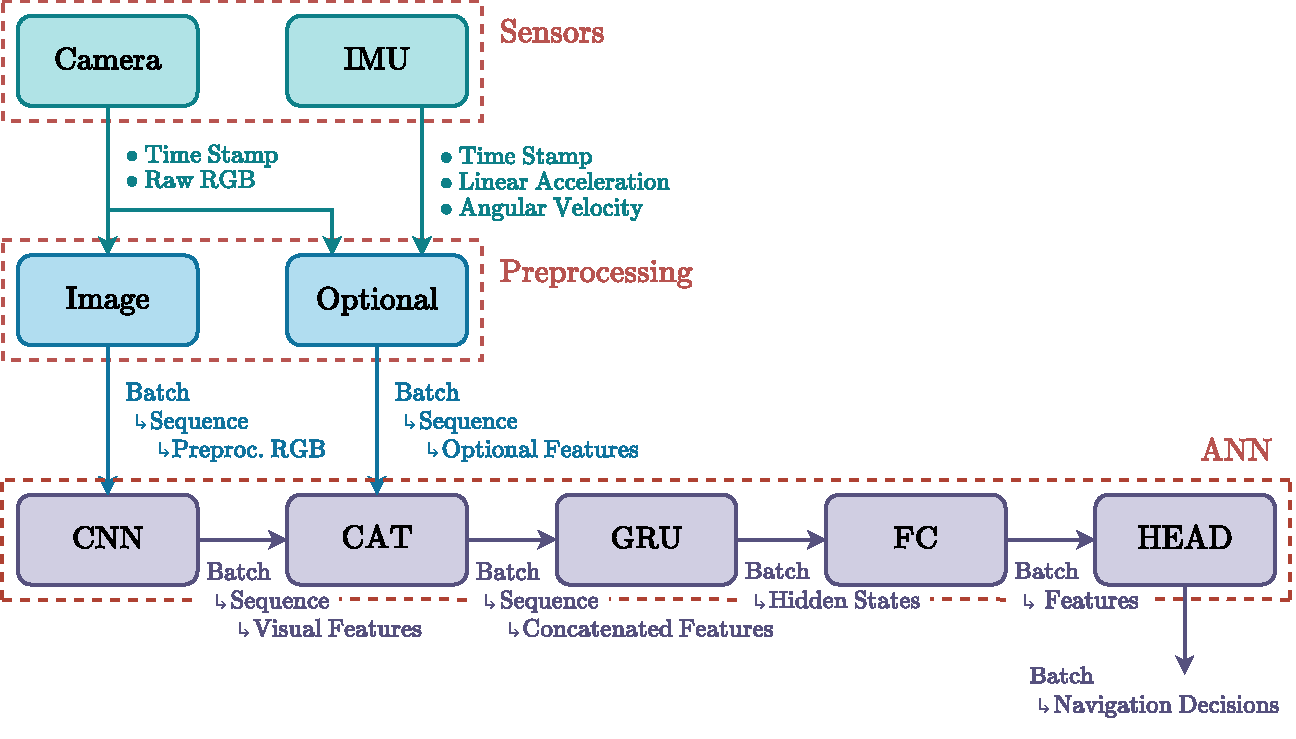
\includegraphics[width=1.0\textwidth]{own/ann_module.drawio.pdf}
    \caption[
        Information flow of the navigation decision making
    ]{
        Information flow of the navigation decision making
    \label{fig:perception_and_reasoning}
    }
\end{figure}


The ANN module learns by
imitation with dataset aggregation
(see section \ref{sec:imitation_learning} for background).
Thereby, the dataset is aggregated from samples demonstrated by the expert
system (see section \ref{sec:expert_system}).
Each sample is a pair of an input sequence and a single lable.
For the individual ANN variant,
the user specifies the sequence length of the samples
\begin{equation} \label{eq:seq_len}
    \seqLen \in \setOfAllPosInts.
\end{equation}
The ANN module is trained on
batches of the aggregated dataset with supervised learning.
The user specifies the batch size
\begin{equation}
    \batchSize \in \setOfAllPosInts.
\end{equation}
The submodules prior to the GRU submodule (CNN and CAT)
have no sequential awareness and, thus, 
process sequence elements in parallel like batch elements.
In contrast, the GRU submodule
operates in many-to-one mode,
whereby each input sequence of feature vectors is mapped to a 
single non-sequential output feature vector.
The subsequent submodules (FC and HEAD)
then process batches of non-sequential data, 
as is common in conventional feedforward networks.
In this sense,
the GRU submodule is mandatory in case the user specifies
$\seqLen > 1$ for the samples of the training dataset.

At racing,
when the autonomous navigation method flies the drone through the racetrack,
the ANN module makes navigation decisions 
in real-time at the user-specified frequency
$\mainFreq$ with the batch size and sequence length 
of the input
$\batchSize = \seqLen =1$.
The GRU submodule (if activated in the specific variant) 
hence operates in one-to-one mode,
i.e., 
each single non-sequential input feature vector
is mapped to a single non-sequential output feature vector.
Since the single input feature vectors 
trace back to the sensor data coming in at a fixed frequency,
they, as a whole, constitute a time series,
on which the GRU submodule can build up memory
% in its hidden state
as learned during the training on the sequences of the specified length.
As a result, both, the current and past sensor data, 
influence the current navigation decision.





%%%%%%%%%%%%%%%%%%%%%%%%%%%%%%%%%%%%%%%
\paragraph*{Input preprocessing} ${}$\\
The drone's onboard camera 
outputs raw RGB images
\begin{equation}
    \rawRGB \in \setOfInts{0, \dots, \rawRGBFullInt}^{
        3 \times \rawRGBHeight \times \rawRGBWidth}
\end{equation}
where 
$\rawRGBFullInt$ (usually $= 255$) is the full pixel intensity 
and
$\rawRGBHeight \times \rawRGBWidth$
is the image size.
The latest raw RGB image is preprocessed in two steps
before being fed to the CNN submodule.
First, the pixel intensities are normalized by the full intensity 
$\rawRGBFullInt$ with the aim
to accelerate the convergence of the loss during training.
Second, the image is sized down 
preserving its aspect ratio
with the user-specified factor $\resizeFact$.
Besides significantly accelerating the training,
this step makes training on longer sequences possible
in the first place by reducing GPU memory usage.
The resulting preprocessed RGB image is
\begin{equation} \label{eq:rgb_preproc}
    \preprocRGB{} \in \setOfInts{\frac{i}{\rawRGBFullInt}}_{
        i \in \setOfInts{0, \dots, \rawRGBFullInt}
    }^{
        3 \times 
        \floor{\resizeFact \cdot \rawRGBHeight} \times 
        \floor{\resizeFact \cdot \rawRGBWidth}
    }
\end{equation} 
where $\floor{\placeholder}$ denotes the operation of rounding down to the nearest integer.



The available optional input features are
\begin{itemize}
    \item the time step
    $\rawRGBTimeStep$
    between the stamps of the raw RGB images processed
    at the previous and the current inference
    \item the latest estimate from the drone's onboard IMU
    (inertial measurement unit) 
    comprising the drone's linear acceleration
    $\IMULinAcc \in \R{3}$
    and angular velocity
    $\IMUAngVel \in \R{3}$
    in the local reference system
    \item the time step
    $\IMUTimeStep$
    between the stamps of the IMU estimates
    processed at the previous and the current inference.
\end{itemize}
The user-activated optional inputs are stacked into the optional input vector
before being fed to the CAT submodule.
For example, the fully activated optional input vector is
\begin{align} \label{eq:opt_inp_vec}
    \optFeatVec{} =
    \begin{bmatrix}
        \rawRGBTimeStep \\
        \IMULinAcc \\
        \IMUAngVel \\
        \IMUTimeStep
    \end{bmatrix}.
\end{align}








%%%%%%%%%%%%%%%%%%%%%%%
\paragraph*{CNN} ${}$\\
The CNN (convolutional neural network) submodule 
extracts visual features of images.
This submodule is implemented with the backbone
of any user-selected TorchVision
classification model\footnote{
    \url{https://pytorch.org/vision/stable/models.html}, visited on 23/08/2022
},
which is obtained by removing the last layer of the model.
In addition, the user specifies whether the backbone
initializes with pretrained weights and whether
the weights of the backbone are trainable.
Since CNN backbones are only applied in this thesis, 
their corresponding mapping is 
regarded as a black box 
\begin{align} \label{eq:CNN}
    \CNNMap 
    :
    \R{\CNNNumC \times \CNNHeight \times \CNNWidth} 
    \rightarrow 
    \R{\CNNOutp}
    ;\quad 
    \img[]{}{}{}{}
    \mapsto 
    \visFeatVec{}
    .
\end{align}
The backbone implementation adapts to the inputted image
in terms of the 
the number of channels $\CNNNumC$,
height $\CNNHeight$
and width $\CNNWidth$.
The backbone's output dimensionality 
$\CNNOutp$
is fixed by the design of its last layer.
The user specifies

The CNN submodule inputs
a batch of sequences of preprocessed RGB images 
(equ. \ref{eq:rgb_preproc}) 
\begin{equation}
    \series{\preprocRGB{t}}_{t \in \setOfInts{1, \dots, \seqLen}, i}
    ,\quad 
    i \in \setOfInts{1, \dots, \batchSize}.
\end{equation}
As it processes the individual sequence elements 
unrelated in parallel like batch elements,
the CNN submodule maps each image of the input batch 
to an individual visual feature vector in the output batch
\begin{equation} \label{eq:cnn_output}
    \series{\visFeatVec{t}}_{t \in \setOfInts{1, \dots, \seqLen}, i}
    ,\quad 
    i \in \setOfInts{1, \dots, \batchSize}.
\end{equation}
The number of trainable parameters $\CNNNumP$ of the CNN submodule 
depends on the user-selected TorchVision model.




%%%%%%%%%%%%%%%%%%%%%%%
\paragraph*{CAT} ${}$\\
The CAT submodule concatenates
two feature vectors
\begin{align} \label{eq:cat}
    \CATMap
    :
    \tuple{\R{\CATInp{1}}, \R{\CATInp{2}}}
    \rightarrow 
    \R{\CATInp{1} + \CATInp{2}}
    ;\quad
    \tuple{\featvec[]{}{1}{}{}, \featvec[]{}{2}{}{}}
    \mapsto
    \begin{bmatrix}
        \featvec[]{}{1}{}{} \\ \featvec[]{}{2}{}{}
    \end{bmatrix}
\end{align}
where the input dimensionalities
$\mathbb{R}^{\num[]{\cat}{1}{}{}}$
and
$\mathbb{R}^{\num[]{\cat}{2}{}{}}$
adapt to the number of features of the input.
This submodule applies to each
visual feature vector 
outputted by the CNN submodule 
(see equ. \ref{eq:cnn_output})
and optional input feature vector
\begin{equation} \label{eq:batch_opt}
    \series{\optFeatVec{t}}_{t \in \setOfInts{1, \dots, \seqLen}, i}
    ,\quad 
    i \in \setOfInts{1, \dots, \batchSize}.
\end{equation}
that correspond to the same position in batch and sequence.
Hence the CAT submodule outputs a batch of sequences
of concatenated feature vectors
\begin{equation} \label{eq:cat_output}
    \series{
        \begin{bmatrix} 
            \visFeatVec{t} \\ \optFeatVec{t}
        \end{bmatrix}
    }_{t \in \setOfInts{1, \dots, \seqLen}, i}
    ,\quad 
    i \in \setOfInts{1, \dots, \batchSize}.
\end{equation}
If the user deactivates all optional inputs,
the CAT submodule also deactivates and recedes to 
the identity map of the the CNN submodule output.
Either way, the CAT submodule has zero trainable parameters
\begin{equation}
    \CATNumP = 0.
\end{equation}




\newcommand{\GRULayerMap}[1]{\Func[]{\gru}{#1}{}{}}
\newcommand{\GRUNumLayer}{\num[\user]{\gru}{\layer}{}{}}
\newcommand{\GRUInp}[1]{\num[]{\gru}{\inp,#1}{}{}}
\newcommand{\GRUHiddenSize}{\num[\user]{\gru}{\hidden}{}{}}

\newcommand{\GRUMap}{\Func[]{\gru}{}{}{}}
\newcommand{\GRUDropout}{\underline\delta}
\newcommand{\GRUDropoutP}{\prob[\user]{\gru}{}{}{}}
\newcommand{\GRUNumP}{\num[]{\gru}{\params}{}{}}

%%%%%%%%%%%%%%%%%%%%%%%
\paragraph*{GRU} ${}$\\
The GRU (gated recurrent unit) submodule
is implemented using the PyTorch
multi-layer GRU\footnote{
    \url{https://pytorch.org/docs/stable/generated/torch.nn.GRU.html}, visited on 24/08/2022
},
which integrates the GRU \cite{Cho2014} 
introduced in section \ref{sec:gru} on each layer.
As a quick reminder, 
the single layer GRU 
has the ability to comprehend temporal relations within sequences.
Each layer 
$l \in \setOfInts{1, \dots, \GRUNumLayer}$ 
processes an input sequence by
iterating through it
$t \in \setOfInts{1, \dots, \seqLen}$ 
mapping the current sequence element
and the layer's previous hidden state
to the current hidden state (see equ. \ref{eq:gru_layer_current_hidden})
\begin{align}
    \GRULayerMap{l}
    :
    \tuple{
        \R{\GRUInp{l}}, 
        \setR{-1, 1}^{\GRUHiddenSize}
    }
    \rightarrow 
    \setR{-1, 1}^{\GRUHiddenSize}
    ;\quad
    \tuple{\featvec[]{(l)}{t}{}{}, \hiddenstate[]{(l)}{t-1}{}{}}
    \mapsto
    \hiddenstate[]{(l)}{t}{}{}.
\end{align}
Thereby, $\hiddenstate[]{(l)}{0}{}{}$ is either initialized with zeros 
or corresponds to the last computed hidden state from the last inference.
 In the multi-layer GRU,
each layer maintains its own hidden state.
The user specifies the number of layers 
$\GRUNumLayer$
and the hidden size 
$\GRUHiddenSize$ (i.e., dimensionality) shared by all hidden states.
While the first GRU layer inputs the elements of the given input sequence,
all subsequent layers input the hidden state from the previous layer subject to dropout
\begin{align} \label{eq:gru}
    \GRUMap
    :\ &
    \tuple{
        \R{\GRUInp{1}},
        \setR{-1, 1}^{\GRUHiddenSize \times \GRUNumLayer}
    }
    \rightarrow 
    \setR{-1, 1}^{\GRUHiddenSize}
    \nonumber \\
    &\tuple{
        \featvec[]{}{t}{}{}, 
        \hiddenstate[]{(1)}{t-1}{}{},
        \dots,
        \hiddenstate[]{(\GRUNumLayer)}{t-1}{}{}
    }
    \mapsto 
    \hiddenstate[]{(\GRUNumLayer)}{t}{}{} =
    \dots
    \nonumber \\
    \dots &\GRULayerMap{\GRUNumLayer} \tuple{
        \GRUDropout \odot
        \GRULayerMap{\GRUNumLayer - 1} \tuple{
            \GRUDropout \odot
                \dots \GRULayerMap{1} \tuple{
                    \featvec[]{}{t}{}{}
                    ,
                    \hiddenstate[]{(1)}{t-1}{}{}
                }
            ,
            \hiddenstate[]{(\GRUNumLayer-1)}{t-1}{}{}
        },
        \hiddenstate[]{(\GRUNumLayer)}{t-1}{}{}
    }
    .
\end{align}
Dropout is a measure that prevents ANNs from overfitting 
to their provided training data.
At training, 
it randomly sets entries of a feature vector to zero 
while maintaining the vector's signal strength on average
in order to force the ANN to learn the extraction of stand-alone features 
whose informative value is independent from the other extracted features \cite{Hinton2012}.
Mathematically, dropout applied on a hidden state (or feature vector)
is calculated with the Hadamard product (denoted with $\odot$)
of that hidden state and the vector $\GRUDropout$ of same dimensionality 
whose entries, for every calculation, 
are random variables resampled 
from a Bernoulli distribution
with a user-specified probability
\begin{equation}
    P \left( \delta_i = 0 \right) = \GRUDropoutP
    ,\quad
    P \left( \delta_i = \frac{1}{1-\GRUDropoutP} \right) = 1 - \GRUDropoutP
    .
\end{equation}
At racing, the dropout probability is null
whereby the dropout is deactivated.

As the $l$-th GRU layer has $3\GRUHiddenSize (\GRUInp{l} + \GRUHiddenSize + 2)$
trainable parameters (see equ. \ref{eq:gru_layer_nparams}),
the total number of trainable parameters of the GRU submodule is
\begin{align} \label{eq:gru_param}
    \GRUNumP = 3\GRUHiddenSize \tuple{
        (\GRUInp{1} + \GRUHiddenSize + 2)
        + 
        (\GRUNumLayer -1)
        (2\GRUHiddenSize + 2)
    }.
\end{align}

The GRU submodule operates in many-to-one mode at training or 
one-to-one mode at racing where the length of the input sequences is one.
Either way, the GRU submodule maps its input batch
(see equ. \ref{eq:cat_output})
to a batch of last hidden states of the last layer
\begin{equation}
    \hiddenstate[]{(\GRUNumLayer)}{\seqLen, i}{}{}
    , \quad i \in \setOfInts{1, \dots, \batchSize}
    .
\end{equation}




\newcommand{\normDesSpeed}{\speed[\norm]{\drone}{\desired}{}{}}
\newcommand{\waypIRS}{\pos[]{\wayp}{}{\irs}{}}
\newcommand{\headNavDec}{(\normDesSpeed, \waypIRS)}

\newcommand{\desAngVel}{\angvel[]{\drone}{\desired}{\lrs}{}}
\newcommand{\desAngAcc}{\angvel[\dot]{\drone}{\desired}{\lrs}{}}
\newcommand{\desColThrust}{\anything[]{\drone}{\desired}{}{}{c}}
\newcommand{\headCtrlCmd}{(\desAngVel, \desAngAcc, \desColThrust)}

\newcommand{\headMap}{\Func[]{\head}{}{}{}}
\newcommand{\headIn}{\num[]{\head}{\inp}{}{}}
\newcommand{\headOut}{\num[]{\head}{\outp}{}{}}
\newcommand{\headMat}{\underline{\underline A}^\head}
\newcommand{\headBias}{\underline{b}^\head}
\newcommand{\headAct}{\func[\user]{\head}{}{}{}}
\newcommand{\headParam}{\num[]{\head}{\params}{}{}}


\newcommand{\fcLayer}{\num[\user]{\fc}{\layer}{}{}}
\newcommand{\fcIn}[1]{\num[]{\fc}{\inp, #1}{}{}}
\newcommand{\fcOut}{\num[\user]{\fc}{\widthh}{}{}}
\newcommand{\fcMap}[1]{\Func[]{\fc}{#1}{}{}}
\newcommand{\fcMat}[1]{\underline{\underline A}^\fc_{#1}}
\newcommand{\fcBias}[1]{\underline{b}^\fc_{#1}}
\newcommand{\fcDropout}{\underline{\delta}^\fc}
\newcommand{\fcAct}{\func[\user]{\fc}{}{}{}}
\newcommand{\fcDropoutProb}{\prob[\user]{\fc}{}{}{}}
\newcommand{\fcParam}{\num[]{\fc}{\params}{}{}}

\subsection*{FC}
The FC submodule performs the function
of increasing the general complexity of the ANN module.
It consists of multiple fully connected layers.
Each layer 
$ l \in \setOfInts{1, \dots, \fcLayer}$ 
applies
an activation, 
dropout
and a biased linear transformation
on the input feature vector
\begin{align} \label{eq:fc_layer}
    \fcMap{l}
    :\ &
    \R{\fcIn{l}} \rightarrow \R{\fcOut}
    ;\quad 
    \featvec[]{}{}{}{} \mapsto
    \fcMat{l} \cdot \fcDropout \odot
    \hadfct{\fcAct} \left(\featvec[]{}{}{}{}\right)
    + \fcBias{l}
    .
\end{align}
In the multi-layer FC submodule, the first layer inputs 
the given input feature vector,
whereas all subsequent layers input the output from the previous layer
\begin{align} \label{eq:fc}
    \fcMap{}
    :\
    \R{\fcIn{1}} \rightarrow \R{\fcOut}
    ;\quad 
    \featvec[]{}{}{}{} \mapsto
    \fcMap{\fcLayer} \tuple{
        \fcMap{\fcLayer - 1} \tuple{
            \dots \fcMap{1} \tuple{
                \featvec[]{}{}{}{}
            }
        }    
    }
    .
\end{align}
For the FC submodule,
the user specifies:
\begin{itemize}
    \item the number of layers $\fcLayer$
    \item the width $\fcOut$, i.e., output dimensionality shared by all layers
    \item the activation function $\fcAct : \R{} \rightarrow \R{}$
    from the non-linear activations implemented in PyTorch\footnote{
        \url{https://pytorch.org/docs/stable/nn.html}, visited on 03/07/2022
    },
    which applies element-wise on the input feature vector (denoted with the overset ${}^\odot$)
    \item the dropout probability $\fcDropoutProb \in \setR{0,1}$,
    i.e., the probability to resample an entry of the vector 
    $\fcDropout$ with zero
    
    
\end{itemize}
The input dimensionality of a layer
adapts to the nuber of features in the given input vector.
For the first layer, it adapts to the feature vector
forwarded to the FC submodule
$\fcIn{1} = \dim \left(\featvec[]{}{}{}{}\right)$.
For all subsequent layers $l \ge 2$,
it adapts to the width of the FC submodule $ \fcIn{l} = \fcOut$.
The biased linear transformation of the $l$-th layer
consists of the multiplication with the matrix of trainable weights
and the addition of the vector of trainable biases
\begin{equation}
    \fcMat{l} \in \R{\fcIn{l} \times \fcOut}
    , \quad
    \fcBias{l} \in \R{\fcOut}
    .
\end{equation}
As a single layer therewith has $\tuple{\fcIn{l} + 1} \fcOut$
trainable parameters,
the total number of trainable parameters of the FC submodule is
\begin{align} \label{eq:fc_param}
    \fcParam = \tuple{
        \fcIn{1} + 1 + 
        \tuple{\fcLayer -1} \tuple{\fcOut +1}
    } \fcOut
    .
\end{align}
The FC submodule maps
the batch of hidden states
outputted by the GRU submodule
to the batch of feature vectors
\begin{equation}
    \fcMap{} \tuple{\hiddenstate[]{}{}{}{}}_i
    , \quad
    i \in \setOfInts{1, \dots, \batchSize}
    .
\end{equation}






\subsection*{HEAD}
The mandatory HEAD submodule
performs the function of mapping
to the final output of the ANN module.
Depending on the user's selection,
the final output is either a navigation decision or a control command.
A navigation decision 
\begin{equation} \label{eq:head_nav_dec}
    \headNavDec
\end{equation}
comprises a normalized desired speed 
$\normDesSpeed \in \setR{0,1}$
of the drone
and a waypoint
$\waypIRS \in \setR{\text{-}1,1}$
in the image reference system
(see fig. \ref{fig:image_reference_system}).
A control command 
\begin{equation} \label{eq:head_ctrl_cmd}
    \headCtrlCmd
\end{equation}
comprises the desired angular velocity
$\desAngVel$
and acceleration
$\desAngAcc$
of the drone in the local reference system 
(see fig. \ref{fig:local_reference_system})
as well as the desired collective thrust 
$\desColThrust$
of the drone's rotors.
In the limited scope of this master's thesis,
the control command output option,
which is a shortcut to the position controller output 
(see section \ref{sec:control_stack}),
is only partly implemented and 
not examined in the experiments in section \ref{maintwo}.

The head submodule
corresponds to a single layer of the FC submodule
without dropout (see equ. \ref{eq:fc_layer})
as it
applies an activation and a biased linear transformation on the
input feature vector
\begin{align} \label{eq:head}
    \headMap
    :\ 
    \R{\headIn}
    \rightarrow 
    \R{\headOut}
    ;\quad 
    \featvec[]{}{}{}{}
    \mapsto
    \headMat \cdot \hadfct{\headAct}\left(\featvec[]{}{}{}{}\right)
    + \headBias
    .
\end{align}
For the HEAD submodule, the user selects
the activation function $\fcAct : \R{} \rightarrow \R{}$
from the non-linear activations implemented in PyTorch\footnote{
        \url{https://pytorch.org/docs/stable/nn.html}, visited on 03/07/2022
    },
which applies element-wise on the input feature vector (denoted with the overset ${}^\odot$).
The input dimensionality adapts to the
number of features of the given input vector
\begin{equation}
    \headIn
    =
    \dim \left(\featvec[]{}{}{}{}\right),
\end{equation}
whereas the output dimensionality
adapts to the user-selected output option
\begin{equation}
    \headOut
    = 
    \begin{cases}
        3
        ,\quad 
        \text{if navigation decision} 
        \\
        7
        ,\quad 
        \text{if control command.} 
    \end{cases}
\end{equation}
The total number of trainable parameters of the HEAD submodule is
\begin{equation} \label{eq:head_param}
    \headParam = \left( \headIn + 1 \right) \headOut
    .
\end{equation}






%CNN: torch vision model, pretrained, trainable, adapt to any RGB size
%CAT: CNN output , CAT input , one vector
%GRU: hidden size, num_layers, bias, dropout
%FC: width, num_layers, act fct, bias
%HEAD: output size, act fct, bias
%GRAPH
%
%loss optimizer learnrate
\subsection*{Output}










\section{Planning module}
The planning module performs the task of path planning
within the autonomous navigation method.
At the user-specified main frequency 
$\freq[\user]{\main}{}{}{}$,
the planning module 
samples states from its local trajectory
and forwards them as reference to the control module.
Every $\num[\user]{\text{plan}}{}{}{}$-th (user-specified) iteration,
the planning module re-computes its local trajectory
on the basis of its input,
i.e., the latest navigation decision and the latest drone state estimate. 
%These trajectories, generated by the planning module, 
%are referred to as local trajectories
%to distinguish them from the expert system's global trajectory
%used when generating training data for the ANN module (see XX).

The latest navigation decision
stems from either the ANN module
(see equ. \ref{eq:head_nav_dec}) 
or, if it has intervened at training data generation,
the expert system (see equ. \ref{eq:nav_dec_by_expert}).
A navigation decision comprises the normalized desired speed 
and the waypoint in the image reference system
\begin{equation}
    (
        \speed[\norm]{\drone}{\desired}{}{}
        ,\ 
        \pos[]{\wayp}{}{\irs}{}
    ).
\end{equation}
The latest drone state estimate stems from the state estimation system.
In simulation, the estimate may correspond to the ground-truth state.
A drone state estimate includes position, velocity and acceleration
with respect to the global reference system
\begin{equation} \label{eq:drone_state}
    \pos[]{\drone}{}{\grs}{}
    ,\ 
    \vel[]{\drone}{}{\grs}{}
    ,\ 
    \acc[]{\drone}{}{\grs}{}.
\end{equation}


At a fraction of the main frequency, i.e.,
$\freq[\user]{\main}{}{}{} / \num[\user]{\text{plan}}{}{}{}$, 
the planning module takes the following 5 steps 
to re-compute its local trajectory.
\begin{enumerate}
    \item Compute the desired speed
    \begin{equation} \label{eq:planning_des_speed}
        \speed[]{\drone}{\desired}{}{}
        = 
        \maxof{
            \speed[\user]{\drone}{\mnm}{}{}
        }{
            \speed[\user]{\drone}{\mxm}{}{}
            \cdot 
            \speed[\norm]{\drone}{\desired}{}{}
        }.
    \end{equation}
    The normalized, desired speed 
    $\speed[\norm]{\drone}{\desired}{}{} \in \left[0, 1\right]$ 
    of the navigation decision
    is rescaled by its upper bound, 
    the user-specified drone's maximum speed 
    $\speed[\user]{\drone}{\mxm}{}{}$.    
    The user-specified drone's minimum speed 
    $\speed[\user]{\drone}{\mnm}{}{}$
    lower-bounds the desired speed.

    \item Compute the drone's distance to the waypoint 
    \begin{equation}
        \dist[]{\dronetowayp}{}{}{}
        = 
        \maxof{
            \dist[\user]{\dronetowayp}{\mnm}{}{}
        }{
            \minof{
                \speed[]{\drone}{\desired}{}{}
                \cdot
                \dur[\user]{\dronetowayp}{}{}{}
            }{
                \dist[\user]{\dronetowayp}{\mxm}{}{}
            }
        }.
    \end{equation}
    The desired speed 
    $\speed[]{\drone}{\desired}{}{}$ 
    is integrated over the user-specified duration
    $\dur[\user]{\dronetowayp}{}{}{}$.
    The result is bounded to the interval spanned 
    by the user-specified minimum
    $\dist[\user]{\dronetowayp}{\mnm}{}{}$
    and maximum
    $\dist[\user]{\dronetowayp}{\mxm}{}{}$
    distance.

    \item Compute the waypoint with respect to the global reference system
    \begin{equation} \label{eq:pl_global_wayp}
        \pos[]{\wayp}{}{\grs}{}
        = 
        \trafo[]{}{\grs\irs}{}{} \left(
            \dist[]{\dronetowayp}{}{}{}
            ,\ 
            \pos[]{\wayp}{}{\irs}{}
        \right).
    \end{equation}
    The transformation
    $\trafo[]{}{\grs\irs}{}{}$
    (see equ. \ref{eq:global_image_transformations})
    backprojects the waypoint
    $\pos[]{\wayp}{}{\irs}{}$ 
    of the navigation decision
    from the 2D image to the 3D global reference system.
    Thereby, the drone's distance 
    $\dist[]{\dronetowayp}{}{}{}$
    to the waypoint
    constitutes the backprojection length.
    
    \item Set the starting time of the local trajectory to the current time
    \begin{equation}
        \timepnt[]{\loctraj}{0}{}{} = t
    \end{equation}
    and compute the duration of the local trajectory 
    \begin{equation}
        \dur[]{\loctraj}{}{}{}
        = 
        \frac{
            \dist[]{\dronetowayp}{}{}{}
        }{
            \minof{
            \speed[]{\drone}{\desired}{}{}
            }{
                %\speed[]{\drone}{}{}{} 
                \left\|
                    \vel[]{\drone}{}{\grs}{}
                \right\|_2
                + 
                \speed[\user]{\drone}{\Delta}{}{}
            }
        }.
    \end{equation}
    The drone's distance 
    $\dist[]{\dronetowayp}{}{}{}$
    to the waypoint is devided 
    by the slower of either the desired speed
    $\speed[]{\drone}{\desired}{}{}$
    or the latest drone speed estimate
    $\left\|\vel[]{\drone}{}{\grs}{}\right\|_2$
    plus a user-specified speed increment
    $\speed[\user]{\drone}{\Delta}{}{}$.
    By relating the desired to the estimated speed,
    excessive speed increases
    potentially violating the drone's dynamic limitations
    can be prevented.

    \item Compute the local trajectory 
    \begin{align} \label{eq:loc_traj}
        \pos[]{\loctraj}{}{\grs}{}
        :\ 
        &\left[0, \dur[]{\loctraj}{}{}{}\right] \rightarrow \mathbb{R}^3
        ;\quad
        %\nonumber \\
        \timepnt[]{}{}{}{}
        \mapsto
        \pos[]{\loctraj}{}{\grs}{}(\timepnt[]{}{}{}{})
    \end{align}
    starting in the latest drone state estimate
    $\pos[]{\drone}{}{\grs}{}
    ,\ 
    \vel[]{\drone}{}{\grs}{}
    ,\ 
    \acc[]{\drone}{}{\grs}{}$
    and ending in the global waypoint
    $\pos[]{\wayp}{}{\grs}{}$
    with unconstrained velocity and acceleration.
    The implementation\footnote{
            \url{https://github.com/markwmuller/RapidQuadrocopterTrajectories}, visited on 17/08/2022
    } 
    of the algorithm of Mueller et. al. \cite{Mueller2013}
    is deployed to find the polynomial trajectory with minimum jerk
    (third time derivative of position)
    by solving the optimization problem
    \begin{align}
        &\qquad \min 
        \int_0^{\dur[]{\loctraj}{}{}{}}
            \left\|
                \pos[\dddot]{\loctraj}{}{\grs}{}(\timepnt[]{}{}{}{})
            \right\|^2_2
        \text d \timepnt[]{}{}{}{}
        \nonumber \\
        \text{s.t.}\quad
        & \pos[]{\loctraj}{}{\grs}{}(0) = \pos[]{\drone}{}{\grs}{}
        \qquad\qquad \pos[]{\loctraj}{}{\grs}{}(\dur[]{\loctraj}{}{}{}) = \pos[]{\wayp}{}{\grs}{}
        \nonumber \\
        & \pos[\dot]{\loctraj}{}{\grs}{}(0) = \vel[]{\drone}{}{\grs}{}
        \qquad\qquad \pos[\dot]{\loctraj}{}{\grs}{}(\dur[]{\loctraj}{}{}{}) \text{ free}
        \nonumber \\
        & \pos[\ddot]{\loctraj}{}{\grs}{}(0) = \acc[]{\drone}{}{\grs}{}
        \qquad\qquad \pos[\ddot]{\loctraj}{}{\grs}{}(\dur[]{\loctraj}{}{}{}) \text{ free}.
    \end{align}
    The drone's dynamic limitations
    are only taken into account in subsequent feasibility checks 
    and are exempt from the above optimization problem.
    This allows the algorithm to solve the optimization problem in closed form
    which is characterized by low computational effort.
    The algorithm therewith qualifies 
    to run at the relatively high frequencies
    required by the autonomous navigation method.
\end{enumerate}


At the main frequency $\freq[\user]{\main}{}{}{}$, 
the planning module takes the following 2 steps to sample 
a reference state from its local trajectory.
\begin{enumerate}
    \item Compute the time point of the reference state
    \begin{equation}
        \timepnt[]{\loctraj}{}{}{} 
        = 
        t - \timepnt[]{\loctraj}{0}{}{} + 1/\freq[\user]{\main}{}{}{}.
    \end{equation}
    The actual time $t$ is related to the starting time 
    $\timepnt[]{\loctraj}{0}{}{}$
    of the local trajectory,
    whose time domain starts at zero.
    The addition of the main period
    $1/\freq[\user]{\main}{}{}{}$
    ensures that the sampled reference state remains prospective at all times.
    \item Sample the current reference state from the local trajectory
    \begin{align} \label{eq:ref_state}
        \pos[]{\text{ref}}{}{\grs}{} 
        &= 
        \pos[]{\loctraj}{}{\grs}{}(\timepnt[]{\loctraj}{}{}{})
        \nonumber \\
        \vel[]{\text{ref}}{}{\grs}{} 
        &= 
        \pos[\dot]{\loctraj}{}{\grs}{}(\timepnt[]{\loctraj}{}{}{})
        \nonumber \\
        \acc[]{\text{ref}}{}{\grs}{} 
        &= 
        \pos[\ddot]{\loctraj}{}{\grs}{}(\timepnt[]{\loctraj}{}{}{})
        \nonumber \\
        \jerk[]{\text{ref}}{}{\grs}{} 
        &= 
        \pos[\dddot]{\loctraj}{}{\grs}{}(\timepnt[]{\loctraj}{}{}{})
        \nonumber \\
        \ang[]{\text{ref}}{z}{}{}
        &=
        \mathrm{atan2}\left(
            \speed[]{\text{ref}}{y}{\grs}{}
            ,
            \speed[]{\text{ref}}{x}{\grs}{}
        \right).
    \end{align}
    The reference yaw $\ang[]{\text{ref}}{z}{}{}$ is set so that
    the drone and therewith its onboard camera 
    point in the direction of flight movement.
\end{enumerate}











\section{Control stack} \label{sec:control_stack}
Within the autonomous navigation method, 
the control stack takes on the task of 
flying the drone as planned.
To do this, the control stack
generates the inputs for the motors attached to the drone's rotors,
which consequently track the latest reference state
(equ. \ref{eq:ref_state})
from the planning module.
In the simulations of this thesis,
the control stack is realized with the RPG Quadrotor Control \footnote{
        \url{https://github.com/uzh-rpg/rpg_quadrotor_control}, visited on 17/08/2022
} implementation
(see figure \ref{fig:control_module}).
Since this thesis centers on the reasoning aspect of autonomous navigation, 
only an overview of the deployed control stack is presented here.
The reader may consult the provided references for more details
on the control.

\begin{figure}
    \centering
    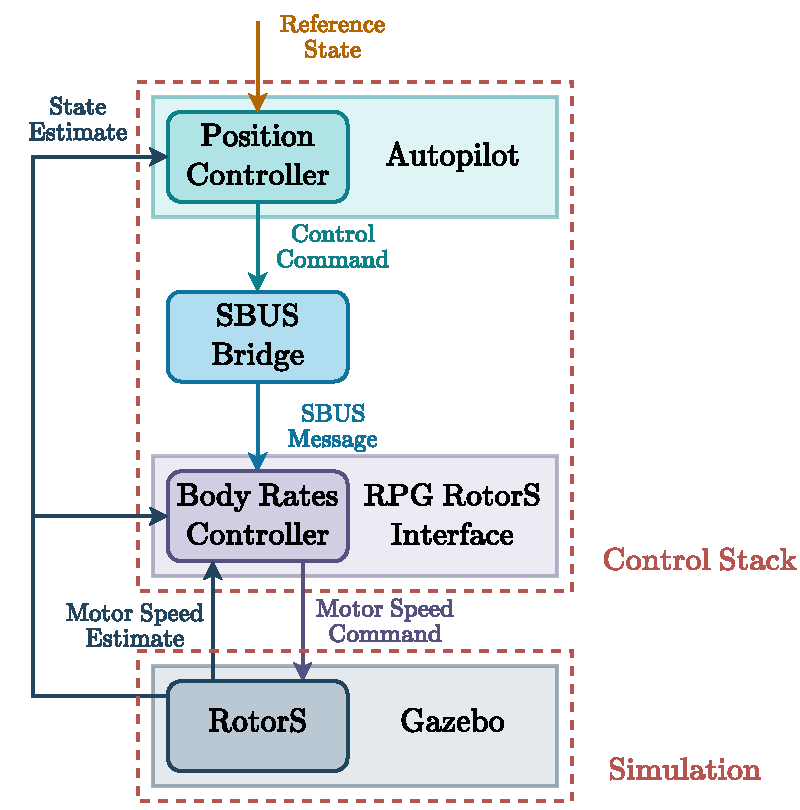
\includegraphics[width=0.7\textwidth]{own/control_module.drawio.pdf}
    \caption[
        The control stack in simulation.
    ]{
        The control stack in simulation.
        \label{fig:control_module}}
\end{figure}

The RPG Quadrotor Control implementation,
which includes the autopilot, the SBUS bridge and and the RPG RotorS interface,
basically executes two feedback control loops in a cascade.
The autopilot integrates the position controller 
that runs the control algorithm of Faessler at al. proposed in \cite{Faessler2018}.
Based on the latest reference state and the fed back drone state estimates,
the position controller generates high-level control commands.
A control command comprises 
the collective thrust of the drone's rotors 
as well as the drone's angular velocity and acceleration.
The SBUS bridge converts each incoming control command
into an SBUS message and forwards this message to the
RPG RotorS interface.
The RPG RotorS interface integrates the body-rate controller
that runs the control algorithm of Faessler at al. proposed in \cite{Faessler2017}.
Based on the latest high-level control command 
as well as the fed back drone state and motor speed estimates,
the body-rate controller generates low-level motor speed commands.
These commands are forwarded to RotorS for execution.
RotorS, developed by Furrer et al. \cite{Furrer2016},
is plugged into the Gazebo \footnote{
    \url{https://gazebosim.org/home}, visited on 18/08/2022
}
simulator to model the drone's physics 
and to provide the controllers with
drone state and motor speed estimates.

In real-world, the drone's flight controller would replace the 
RPG RotorS interface in order to generate hardware-specific low-level
motor commands based on the latest SBUS message from the SBUS bridge.








\section{Expert system} \label{sec:expert_system}
%In contrast to the ANN module,
%the expert system derives its navigation decisions 
%not from onboard sensor data but from its knowledge base.
%The task of the ANN module 
%is to infer navigation decisions,
%i.e., the inputs of the planning module,
%from onboard sensor data.
%In order to make meaningful decisions
%that successfully guide the drone through the racetrack,
%the ANN module must be previously trained on training data 
%of sufficient quantity and quality.
%To guarantee both,
%the training data is automatically generated 
%while the drone is flying through the racetrack.
%At training data generation (see XXX),
%the expert system undertakes the task
%of the completely untrained or yet insufficiently trained ANN module
%to make navigation decisions.

In the context of machine learning, 
an expert system is a program that imitates a human expert
in order to solve a problem. 
It comprises a knowledge base,
which stores known facts and rules, and an
inference engine, which infers new facts 
by applying the rules to the known facts \cite{osti_5675197}.

\paragraph*{Problem} $\ $\\
This thesis implements the expert system 
by Kaufmann et al. \cite{Kaufmann2018}
in order to solve the problem of automated navigation decision making
during the generation of training data for the ANN module.
The training dataset is extended with new samples 
while the drone runs the autonomous navigation method to fly through a racetrack.
The expert system checks the latest navigation decision 
made by the yet partially trained ANN module.
If it does not meet certain requirements,
the expert system intervenes with its own navigation decision.
This, first, keeps the drone on course and, second,
triggers the generation of a new training sample labeled 
with the expert system's navigation decision.

\paragraph*{Knowledge base} $\ $\\
While the ANN module infers navigation decisions from onboard sensor data,
the expert system makes navigation decisions based on its knowledge
which includes the following known facts (\textbf{F*}) and rules (\textbf{R*}).
\begin{itemize}
    
    \item [\textbf{F1}] 
    The planning module's waypoint
    \begin{equation}
        \pos[]{\text{ann}}{\wayp}{\grs}{}
    \end{equation}
     with respect to the global reference system
    (see equ. \ref{eq:pl_global_wayp}) 
    that was computed based
    on the ANN module's latest navigation decision
    (see equ. \ref{eq:head_nav_dec}).
    

    \item [\textbf{F2}] The drone's latest position and quaternion orientation estimate,
    which are provided by the drone's state estimation system and 
    may correspond to ground truth in the simulation
    \begin{equation}
        \pos[]{\drone}{}{\grs}{}
        ,\quad 
        \quat[]{\drone}{}{\grs}{}.
    \end{equation}
    
    \item [\textbf{F3}] The center points of the gates of the racetrack
    \begin{equation}
        \left( 
            \pos[]{\gate}{\idx[]{}{}{}{}}{\grs}{}
        \right)
        _{\idx[]{}{}{}{} \in \left\{0, ..., \num[]{\gate}{}{}{} - 1 \right\}}
    \end{equation}
    and the initial index to the currently targeted gate to be passed next
    \begin{equation}
        \idx[]{\gate}{\target}{}{} \in \left\{0, ..., \num[]{\gate}{}{}{} - 1 \right\}
        .
    \end{equation}

    \item [\textbf{R1}] Compute the global trajectory of the current racetrack
    \begin{align} \label{eq:glo_traj}
        \pos[]{\glotraj}{}{\grs}{}
        :\ 
        &\left[
            \timepnt[]{\gate}{0}{}{}, 
            \timepnt[]{\gate}{\num[]{\gate}{}{}{}}{}{}
        \right] \rightarrow \mathbb{R}^3
        ;\quad
        \timepnt[]{}{}{}{}
        \mapsto
        \pos[]{\glotraj}{}{\grs}{}(\timepnt[]{}{}{}{})
        .
    \end{align}
    The algorithm of Mellinger and Kumar \cite{Mellinger2011}
    finds the minimum snap (fourth time derivative of position) spline trajectory
    \begin{align}
        \pos[]{\glotraj}{}{\grs}{}(\timepnt[]{}{}{}{})
        = \sum_{i = 0}^{\num[]{\gate}{}{}{} - 1}
        \begin{cases}
            \pos[]{\glotraj}{i}{\grs}{}(\timepnt[]{}{}{}{})
            , 
            &t \in \left[\timepnt[]{\gate}{i}{}{}, \timepnt[]{\gate}{i+1}{}{}\right] \\
            0, & \text{else}
        \end{cases}
    \end{align}
    that, traverses through all gate center points (\textbf{F3}),
    each at its corresponding gate time $\timepnt[]{\gate}{i}{}{}$,
    and reconnects to itself at $t=\timepnt[]{\gate}{\num[]{\gate}{}{}{}}{}{}$ at gate $i=0$.
    The entries of the pieces 
    $\pos[]{\glotraj}{i}{\grs}{}(\timepnt[]{}{}{}{})$
    of the spline are polynomials. 
    The user specifies the polynomial order 
    $\num[\user]{\glotraj}{\text{poly}}{}{}$
    of the pieces and
    the continuity order
    $\num[\user]{\glotraj}{\text{cont}}{}{}$
    of the spline. 
    However, since the goal is to minimize snap,
    it is required that 
    $
    \num[\user]{\glotraj}{\text{poly}}{}{}
    \ge \num[\user]{\glotraj}{\text{cont}}{}{} \ge 4
    $.
    The algorithm performs the following two-step iterative optimization.

    First,
    the optimal polynomial coefficients of the spline pieces
    are found for fixed gate arrival times 
    $\timepnt[]{\gate}{i}{}{}$
    by solving the optimization problem
    \begin{align}
        &\qquad \argmin{\pos[]{\glotraj}{}{\grs}{}}
        \int_{\timepnt[]{\gate}{0}{}{}}^{\timepnt[]{\gate}{\num[]{\gate}{}{}{}}{}{}}
            \left\|
                \pos[\ddddot]{\glotraj}{}{\grs}{}(\timepnt[]{}{}{}{})
            \right\|^2_2
        \text d \timepnt[]{}{}{}{}
        \nonumber 
        \\
        \text{s.t.}\quad
        & \pos[]{\glotraj}{}{\grs}{}\left(\timepnt[]{\gate}{i}{}{}\right) = 
            \pos[]{\gate}{\idx[]{}{}{}{}}{\grs}{},
        &&
            \frac{\text d^j \pos[]{\glotraj}{}{\grs}{}}{\text d \timepnt[]{j}{}{}{}} 
            (\timepnt[]{\gate}{i}{}{}) \text{ defined},
        \nonumber \\
        & \idx[]{}{}{}{} \in \left\{0, ..., \num[]{\gate}{}{}{}\right\},
        && j \in \left\{1, ..., \num[\user]{\glotraj}{\text{cont}}{}{}\right\}.
    \end{align}
    Note that, as the spline is closed, 
    the first and last gate equate 
    $\pos[]{\gate}{\num[]{\gate}{}{}{}}{\grs}{} = \pos[]{\gate}{0}{\grs}{}$.
    Morover, the gate times of the very first iteration are 
    approximated with the distances between the gate center points
    devided by the user-specified maximum speed $\speed[\user]{\glotraj}{\mxm}{}{}$ of the trajectory.
    The above optimization problem
    is temporally and spatially dedimensionalized 
    to increase numeric stability and 
    reformulated as quadratic program,
    which is solved with the Gurobi\footnote{
        \url{https://www.gurobi.com/}, visited on 20/08/2022
    } optimizer.

    Second, the polynomial coefficients of the spline pieces 
    are fixed
    and the inner gate times
    $\timepnt[]{\gate}{i}{}{}$
    are optimized relatively to each other.
    The corresponding optimization problem
    \begin{align}
        &\qquad \argmin{\timepnt[]{\gate}{i}{}{}}
        \int_{\timepnt[]{\gate}{0}{}{}}^{\timepnt[]{\gate}{\num[]{\gate}{}{}{}}{}{}}
            \left\|
                \pos[\ddddot]{\glotraj}{}{\grs}{}(\timepnt[]{}{}{}{})
            \right\|^2_2
        \text d \timepnt[]{}{}{}{}
        \nonumber \\
        \text{s.t.}\quad
        & \timepnt[]{\gate}{i}{}{} < \timepnt[]{\gate}{i+1}{}{},
        \qquad
        \timepnt[]{\gate}{0}{}{},\ \timepnt[]{\gate}{\num[]{\gate}{}{}{}}{}{} \text{ fixed},
        \qquad
        \idx[]{}{}{}{} \in \left\{0, ..., \num[]{\gate}{}{}{} - 1 \right\}
    \end{align}
    is solved by gradient descent with backtracking line search.

    
    
    The two optimization steps are executed iteratively until the cost
    of the first optimization problem converges. 
    Then, the trajectory is temporally and spatially redimensionalized
    and temporally scaled to adhere to 
    the user-specified maximum values in terms of 
    speed
    $\speed[\user]{\glotraj}{\mxm}{}{}$, 
    thrust 
    $\scacc[\user]{\glotraj}{\mxm}{}{}$
    and roll-pitch rate 
    $\scangvel[\user]{\glotraj}{\mxm}{}{}$
    along the trajectory. 
    For later use,
    the expert system samples the positions and speeds
    of the global trajectory
    \begin{equation}
        \left( 
            \pos[]{\glotraj}{\idx[]{}{}{}{}}{\grs}{}
        \right)
        _{\idx[]{}{}{}{} \in \left\{0, ..., \num[]{\glotraj}{}{}{} - 1 \right\}}
        ,\quad
        \left( 
            \speed[]{\glotraj}{\idx[]{}{}{}{}}{\grs}{}
        \right)
        _{\idx[]{}{}{}{} \in \left\{0, ..., \num[]{\glotraj}{}{}{} - 1 \right\}}
    \end{equation}
    with $\speed[]{\glotraj}{\idx[]{}{}{}{}}{\grs}{} = 
    \left\| 
        \pos[\dot]{\glotraj}{\idx[]{}{}{}{}}{\grs}{}
    \right\|_2 $.
    The sampling occurs at the
    user-specified frequency
    $\freq[\user]{\glotraj}{}{}{}$,
    which results in
    $\num[]{\glotraj}{}{}{} = \freq[\user]{\glotraj}{}{}{} \cdot 
    \left(\timepnt[]{\gate}{\num[]{\gate}{}{}{}}{}{}
    - \timepnt[]{\gate}{0}{}{}\right)$
    samples.

    
    \item [\textbf{R2}] If the drone is closer to the currently targeted gate 
    than a user-specified distance
    \begin{equation}
        \left\| 
            \pos[]{\gate}{\idx[]{\gate}{\target}{}{}}{\grs}{} - \pos[]{\drone}{}{\grs}{}
        \right\|_2 
        < 
        \dist[\user]{\dronetogate}{}{}{},
    \end{equation}
    increment the index to the currently targeted gate
    \begin{align}
        \idx[]{\gate}{}{}{} &\leftarrow (\idx[]{\gate}{}{}{} + 1) \bmod \num[]{\gate}{}{}{}.
    \end{align}
    
    \item [\textbf{R3}] If the
    planning module's waypoint (\textbf{F1}) computed based on the
    ANN module's latest navigation decision,
    is more distant from the global trajectory (\textbf{R1}) than
    a user-specified margin scaled by the 
    the user-specified drone's maximum speed, i.e.,
    \begin{equation}
        \argmin{i \in \{0, ..., \num[]{\glotraj}{}{}{} - 1\}}
            \left\| 
                \pos[]{\text{ann}}{\wayp}{\grs}{}
                - 
                \pos[]{\glotraj}{i}{\grs}{}
            \right\|_2
            >
            \dist[\user]{\wayptoglotraj}{\mxm}{}{} \cdot \frac{\speed[\user]{\drone}{\mxm}{}{} +1}{5},
    \end{equation}
    the expert system is required to intervene with its own navigation decision.

    
    \item [\textbf{R4}] Update the index 
    $\idx[]{\glotraj}{\proj}{}{} \in \{0, ..., \num[]{\glotraj}{}{}{} - 1\}$ 
    to the projection state,
    i.e., the state of the global trajectory
    onto which the drone's latest position estimate is projected,
    with the following iterative method.
    Figure \ref{fig:expert_system_projection} 
    schematically illustrates the method with a 2D example.
    \begin{enumerate}
        \item Compute the index to the previous state of the global trajectory,
        by decrementing the index to the projection state
        \begin{equation}
            \idx[]{\glotraj}{\prev}{}{} 
            = 
            (\idx[]{\glotraj}{\proj}{}{} - 1 + \num[]{\glotraj}{}{}{}) 
            \bmod 
            \num[]{\glotraj}{}{}{}.
        \end{equation}
        \item Starting from the previous state, 
        compute the vector to the projection state
        \begin{equation} \label{eq:vec_prev_state_2_proj_state}
            \anything[]{}{}{\grs}{}{\underline a}
            = 
            \pos[]{\glotraj}{\idx[]{\glotraj}{\proj}{}{}}{\grs}{}
            - 
            \pos[]{\glotraj}{\idx[]{\glotraj}{\prev}{}{}}{\grs}{}
        \end{equation}
        and the vector to the current drone position
        \begin{equation} \label{eq:vec_prev_state_2_drone}
            \anything[]{}{}{\grs}{}{\underline b}
            = 
            \pos[]{\drone}{}{\grs}{}
            - 
            \pos[]{\glotraj}{\idx[]{\glotraj}{\prev}{}{}}{\grs}{}.
        \end{equation}
        \item If the scalar product of the vectors 
        $\anything[]{}{}{\grs}{}{\underline a}$ 
        and 
        $\anything[]{}{}{\grs}{}{\underline b}$, 
        both normalized by the length of $\anything[]{}{}{\grs}{}{\underline a}$,
        is less than 1
        \begin{align} \label{eq:norm_dot_prod_criterion}
            \frac{
                \anything[]{}{}{\grs}{}{\underline a} 
                \cdot 
                \anything[]{}{}{\grs}{}{\underline b}
            }{  
                \anything[]{}{}{\grs}{}{\underline a} 
                \cdot 
                \anything[]{}{}{\grs}{}{\underline a}
            } < 1,
        \end{align}
        go to the next step. 
        Else, increment the index to the projection state
        \begin{equation}
            \idx[]{\glotraj}{\proj}{}{} 
            \leftarrow 
            (\idx[]{\glotraj}{\proj}{}{} + 1) \bmod \num[]{\glotraj}{}{}{}
        \end{equation}
        and go back to step 1.
        \item If the drone is 
        within a user-specified distance to the projection state 
        \begin{equation} \label{eq:dist_drone_proj_criterion}
            \left\| 
                \pos[]{\drone}{}{\grs}{}
                - 
                \pos[]{\glotraj}{\idx[]{\glotraj}{\proj}{}{}}{\grs}{}
            \right\|_2 
            \le 
            \dist[\user]{\dronetoproj}{}{}{},
        \end{equation}
        the index 
        $\idx[]{\glotraj}{\proj}{}{}$ 
        to the projection state is found.
        Else, set the index 
        to the state of the global trajectory
        which has the minimum distance to the current drone position
        \begin{equation} \label{eq:proj_idx_with_min_dist}
            \argmin{\idx[]{\glotraj}{\proj}{}{}}
            \left\| 
                \pos[]{\drone}{}{\grs}{}
                - 
                \pos[]{\glotraj}{\idx[]{\glotraj}{\proj}{}{}}{\grs}{}
            \right\|_2.
        \end{equation}
        Due to this step,
        the expert system does not require to know
        the initial index 
        to the projection state.

    \end{enumerate}
    
    

    \begin{figure}
        \centering
        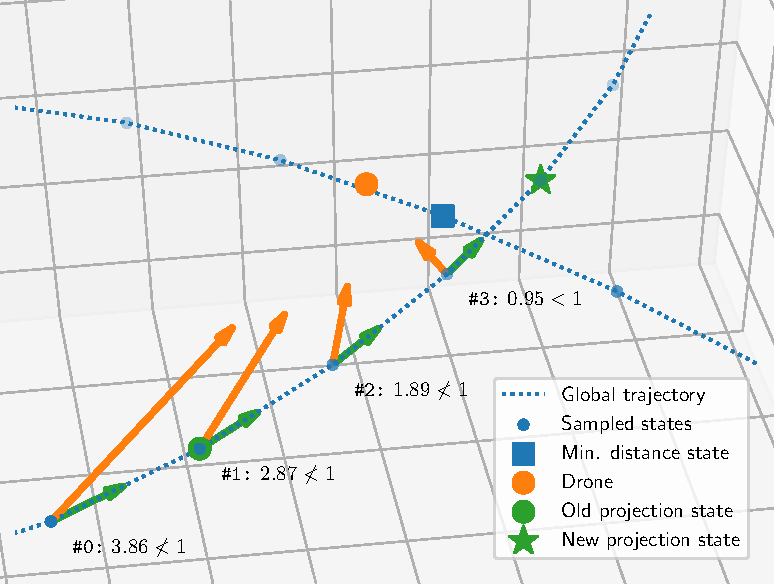
\includegraphics[width=0.9\textwidth]{own/expert_state_projection_3d.pdf}
        \caption[
            Update of the projection state index
        ]{
            Schematic example
            of the update of the projection state index (\textbf{R4}).
            Known are: the positions (blue points) 
            sampled from the global trajectory (blue dotted line),
            the last index to the projection state (green circle)
            and the current position of the drone (orange circle).
            At an iteration,
            the vector from the previous to the projection state 
            (green arrows, equ. \ref{eq:vec_prev_state_2_proj_state})
            and the vector from the previous to the drone position 
            (orange arrows, equ. \ref{eq:vec_prev_state_2_drone})
            are computed.
            Then, the normalized dot product criterion 
            (annotations, equ. \ref{eq:norm_dot_prod_criterion}) 
            is checked. 
            For iteration \#0-2, the criterion is not met.
            Thus, the index to the projection state is incremented
            and another iteration is started.
            At iteration \#3 the criterion is met and the 
            new index to the projection state (green star) is identified
            (assuming the distance criterion 
            (equ. \ref{eq:dist_drone_proj_criterion}) is also met). 
            Note that finding the index to the projection state 
            only with minimum distance 
            (equ. \ref{eq:proj_idx_with_min_dist}) 
            would have failed here,
            since the so indexed state (blue square) 
            belongs to a later or earlier part of the global trajectory 
            which only intersects the current part.
        \label{fig:expert_system_projection}}
    \end{figure}


    
    \item [\textbf{R5}] 
    Update the index 
    $\idx[]{\glotraj}{v}{}{} \in \{0, ..., \num[]{\glotraj}{}{}{} - 1\}$
    to the speed state,
    i.e., the state of the global trajectory
    that is the reference for the normalized speed
    $\speed[\norm]{\expert}{\desired}{}{}$ component
    of the expert system's navigation decision,
    by finding the first state of the global trajectory 
    that follows the projection state
    with a specific distance.
    \begin{enumerate}
        \item Initialize the searched index with the index to the projection state
        \begin{equation}
            \idx[]{\glotraj}{v}{}{} = \idx[]{\glotraj}{\proj}{}{}.
        \end{equation}

        \item Increment the searched index
        \begin{equation}
            \idx[]{\glotraj}{v}{}{} \leftarrow (\idx[]{\glotraj}{v}{}{} + 1) \bmod \num[]{\glotraj}{}{}{}.
        \end{equation}
        \item If the speed state is further 
        from the projection state than a user-specified distance
        \begin{equation}
            \left\| 
                \pos[]{\glotraj}{\idx[]{\glotraj}{v}{}{}}{\grs}{}
                - 
                \pos[]{\glotraj}{\idx[]{\glotraj}{\proj}{}{}}{\grs}{}
            \right\|_2
            > 
            \dist[\user]{\projtospeed}{}{}{}
            .
        \end{equation}
        the searched index is found.
        Else, go back to step 2.
    \end{enumerate}


    \item [\textbf{R6}] 
    Update the index 
    $\idx[]{\glotraj}{\wayp}{}{} \in \{0, ..., \num[]{\glotraj}{}{}{} - 1\}$
    to the waypoint state,
    i.e., the state of the global trajectory
    that is the reference for the image waypoint
    $\pos[]{\expert}{\wayp}{\irs}{}$
    component of the expert system's navigation decision,
    by finding the first state of the global trajectory 
    that follows the projection state
    with a distance to be computed.
    \begin{enumerate}
        \item Set the distance from the projection to the waypoint state
        to the distance from the drone to the closer of
        either the currently or lastly targeted gate.
        However, a user-specified distance constitutes the lower limit
        \begin{align}
            \dist[]{\projtowayp}{}{}{} &= 
            \maxof{
                \dist[\user]{\projtowayp}{\mnm}{}{}
            }{
                \argmin{i} \left\| 
                    \pos[]{\gate}{i}{\grs}{} 
                    - 
                    \pos[]{\drone}{}{\grs}{}
                \right\|_2
            }, 
            \\
            i &\in \left\{ \idx[]{\gate}{\target}{}{}, 
            (\idx[]{\gate}{\target}{}{} - 1 + \num[]{\gate}{}{}{}) 
            \bmod 
            \num[]{\gate}{}{}{}
            \right\}
            .
        \end{align}
        \item Initialize the searched index with the index to the projection state
        \begin{equation}
            \idx[]{\glotraj}{\wayp}{}{} = \idx[]{\glotraj}{\proj}{}{}.
        \end{equation}
        \item Increment the searched index
        \begin{equation}
            \idx[]{\glotraj}{\wayp}{}{} \leftarrow (\idx[]{\glotraj}{\wayp}{}{} + 1) 
            \bmod \num[]{\glotraj}{}{}{}.
        \end{equation}
        \item If the waypoint state is further from the projection state 
        than the distance computed in step 1
        \begin{equation}
            \left\| 
                \pos[]{\glotraj}{\idx[]{\glotraj}{\wayp}{}{}}{\grs}{}
                - 
                \pos[]{\glotraj}{\idx[]{\glotraj}{\proj}{}{}}{\grs}{}
            \right\|_2
            > 
            \dist[]{\projtowayp}{}{}{},
        \end{equation}
        the searched index is found.
        Else, go back to step 3.
    \end{enumerate}


    


    \item [\textbf{R7}] Compute the normalized speed component
    of the expert system's navigation decision
    as the sampled speed of the speed state
    normalized by the maximum speed of the global trajectory
    \begin{equation}
        \speed[\norm]{\expert}{\desired}{}{}
        = 
        \frac{
            \speed[]{\glotraj}{\idx[]{\glotraj}{v}{}{}}{\grs}{}
        }
        {
            \argmax{i \in \{0, ..., \num[]{\glotraj}{}{}{} - 1\}}
            \left\| 
                \speed[]{\glotraj}{\idx[]{}{}{}{}}{\grs}{}
            \right\|_2
        }  
        \in [0,1].
    \end{equation}


    
    
    
    \item [\textbf{R8}] Compute the image waypoint component
    of the expert system's navigation decision
    by applying the transformation
    from the global to the image reference system (see equ. \ref{eq:global_image_transformations})
    on the sampled position of the waypoint state 
    \begin{equation}
        \pos[]{\expert}{\wayp}{\irs}{}
        =
        \trafo[]{}{\irs\grs}{}{} \left(
            \pos[]{\glotraj}{\idx[]{\glotraj}{\wayp}{}{}}{\irs}{}
        \right)
        .
    \end{equation}

\end{itemize}





\paragraph*{Inference Engine} $\ $\\
The inference engine of the expert system is only activated 
during training data generation.
Figure ?? shows the related interaction of the inference engine 
within the autnomous navigation method.
Internally, the inference engine runs the following schedule.

Before the drone starts to fly,
the inference engine pre-computes the global trajectory (\textbf{R1})
and samples the position and speeds.
During the flight, it constantly update the currently targeted
gate index (\textbf{R2}).
Whenever the planning module has computed a global waypoint on the basis
of the latest ANN navigation decision,
the inference engine checks whether it must intervene (\textbf{R3}).
If so, the engine updates its indices to relevant states of the global trajectory
(\textbf{R4-6})
and makes its own navigation decision (\textbf{R7-8}).
Finally the engine sends its navigation decision to the planning module for processing.

\section{Racing vs. Training Data Generation}






\chapter{Experiments in Simulation}
\label{maintwo}

\section{Simulation Setup} \label{sec:sim_setup}
The experiments in this thesis 
are conducted in a drone racing simulation,
which includes the environment, 
the racetrack consisting of race gates 
and the drone.
The implementation of the simulation (see fig. \ref{fig:simulation_setup})
is separated into physics modeling and image rendering.
\begin{figure}%[h]
    \centering
    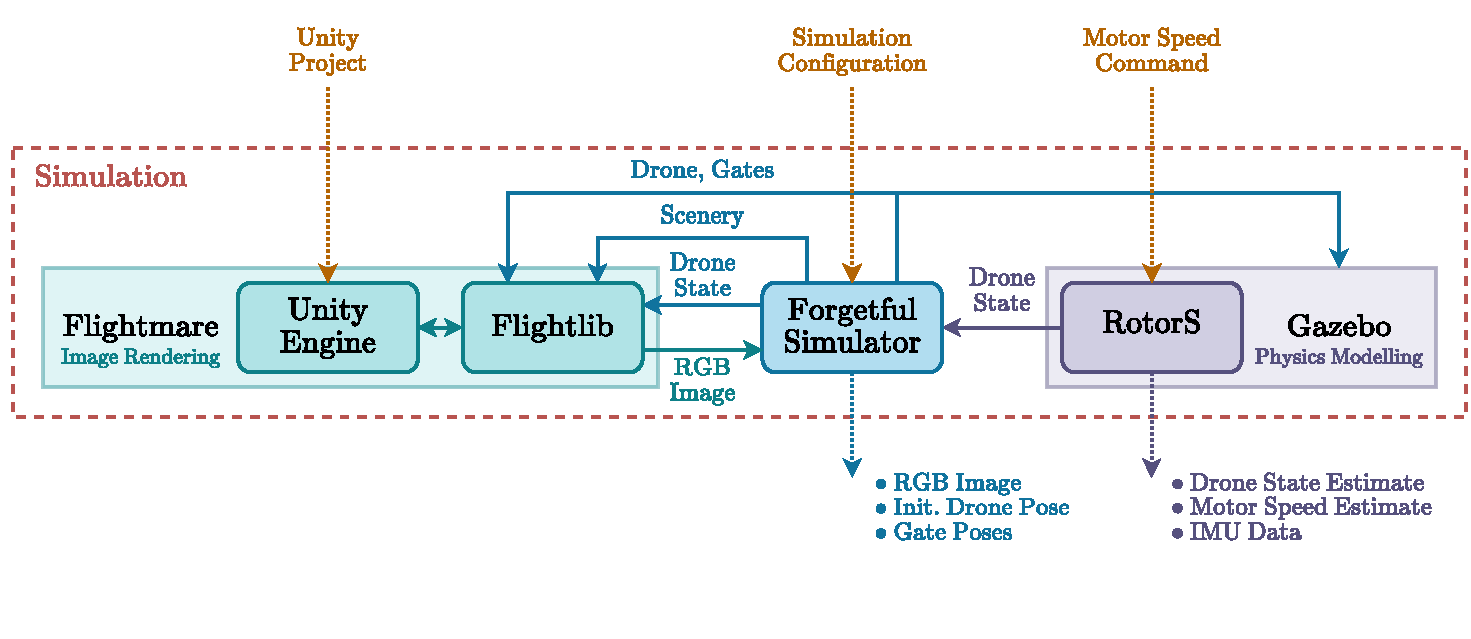
\includegraphics[width=1.0\textwidth]{own/simulation_setup.drawio.pdf}
    \caption[
        Implementation concept of the simulation
    ]{
        Implementation concept of the simulation
    \label{fig:simulation_setup}
    }
\end{figure}

For a physics modeling of high accuracy,
the Gazebo\footnote{\url{https://gazebosim.org/home}, accessed on \today} 
simulator
with the RotorS \cite{Furrer2016} plugin is deployed.
The modeling includes the dynamics of the drone under 
the actuation with inputted motor speed commands
and possible collisions of the drone with the racetrack gates.
Further, the RotorS plugin provides the
drone state estimate, the motor speeds estimate and the
data from the onboard IMU as output.


For an almost photo-realistic image rendering,
the Flightmare \cite{Song2020} simulator 
is deployed.
Upon request, the Flightlib interface
updates the drone pose 
within the Unity\footnote{
    \url{https://unity.com/}, accessed on \today
} Engine
and fetches an RGB image from the drone's onboard camera.
Before running the simulation,
the Unity Engine is built from a Unity project
that bases on the RPG Flightmare Unity Project\footnote{
    \url{https://github.com/uzh-rpg/flightmare_unity}, accessed on \today
}.
The Unity project of this thesis
entails five scenes
named
spaceship interior\footnote{
    based on "3D Free Modular Kit" from the Unity Asset Store
},
destroyed city\footnote{
    based on "Destroyed City FREE" from the Unity Asset Store
},
industrial site\footnote{
    based on "RPG/FPS Game Assets for PC/Mobile (Industrial Set v2.0)" from the Unity Asset Store
},
polygon city\footnote{
    based on "CITY package" from the Unity Asset Store
}
and desert mountain\footnote{
    based on "Free Island Collection" from the Unity Asset Store
}
(see fig. \ref{fig:unity_scenes}).
The scenes base on assets from the Unity Asset Store\footnote{
    \url{https://assetstore.unity.com/}, accessed on \today
}.
Within each scene, there are three sites (A, B, C) to place a racetrack.
For the racetrack, two different gate types are provided:
the first with TU Berlin/DAI-Labor logos and 
the second with Tsinghua University/DME logos
(see fig. \ref{fig:unity_gates}).
\begin{figure}
    \centering
    \subfloat[
        Spaceship Interior
    ]{
        \label{fig:unity_scene_SI}
        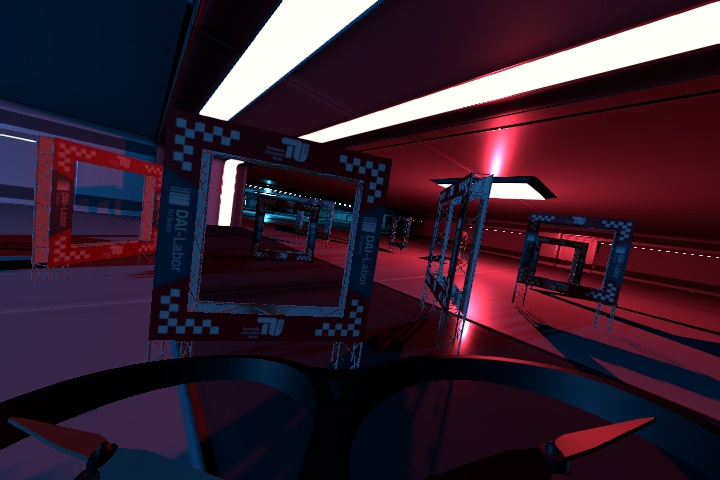
\includegraphics[width=0.33\textwidth]{own/jpg/spaceship_interior.jpg}
    }
    %\hspace*{0cm}                
    \subfloat[
        Destroyed City
    ]{
        \label{fig:unity_scene_DC}
        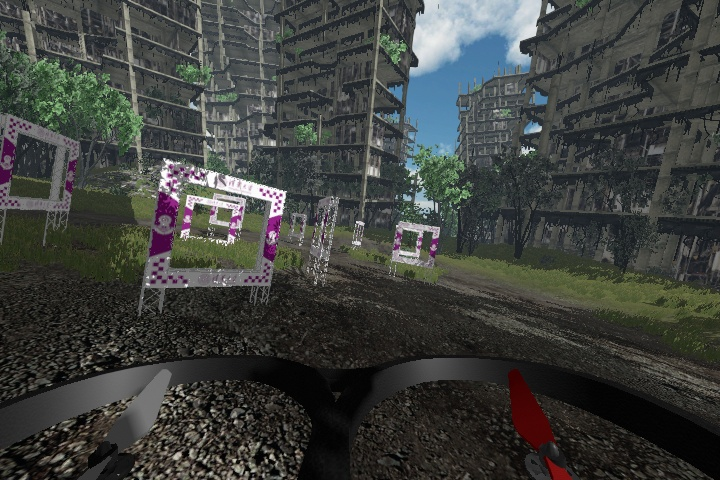
\includegraphics[width=0.33\textwidth]{own/jpg/destroyed_city.jpg}
    }
    \par
    \subfloat[
        Industrial Site
    ]{
        \label{fig:unity_scene_IS}
        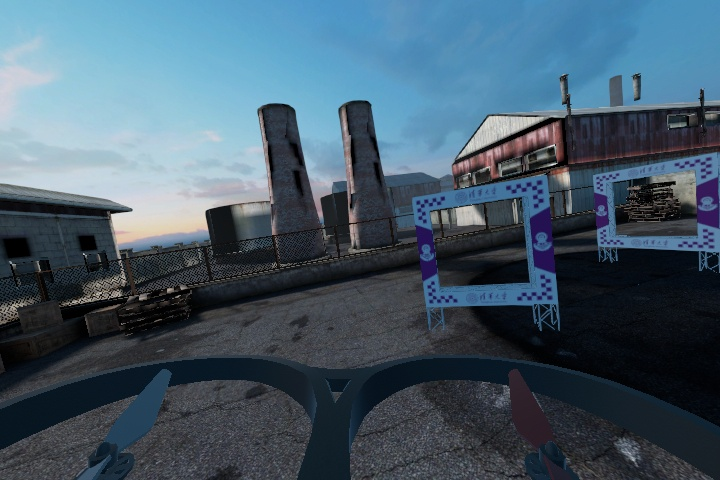
\includegraphics[width=0.33\textwidth]{own/jpg/industrial_site.jpg}
    }
    \subfloat[
        Polygon City
    ]{
        \label{fig:unity_scene_PC}
        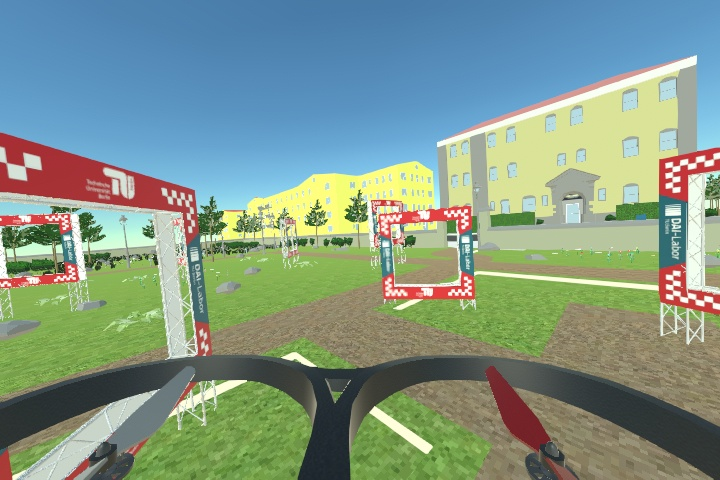
\includegraphics[width=0.33\textwidth]{own/jpg/polygon_city.jpg}
    }
    \subfloat[
        Desert Mountain
    ]{
        \label{fig:unity_scene_DM}
        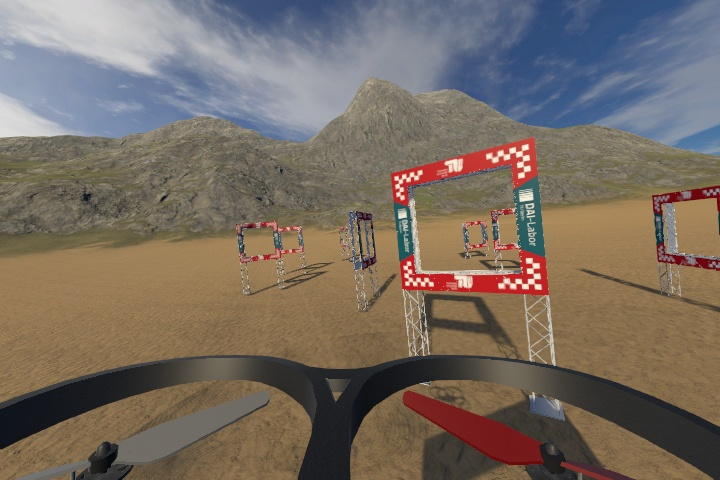
\includegraphics[width=0.33\textwidth]{own/jpg/desert_mountain.jpg}
    }
    \caption[
        Scenes available in simulation
    ]{
        Scenes available in simulation
        \label{fig:unity_scenes}
    }
\end{figure}
\begin{figure}[h]
    \centering
    \subfloat[
        DAI-Labor at TU Berlin
    ]{
        %\label{fig:unity_scene_SI}
        
\includegraphics[width=0.33\textwidth]{own/jpg/tub_dai_gate.png}
    }       
    \subfloat[
        DME at Tsinghua University
    ]{
        %\label{fig:unity_scene_DC}
        
\includegraphics[width=0.33\textwidth]{own/jpg/thu_dme_gate.png}
    }
    \caption[
        Race gates available in simulation
    ]{
        Race gates available in simulation
        \label{fig:unity_gates}
    }
\end{figure}

The Forgetful Simulator node takes on two tasks.
First, it synchronizes the
drone state in the Flightmare simulator with the
ground-truth state in the Gazebo simulator and 
provides the RGB images fetched from the Flightmare simulator
as output.
Second, the node sets up the simulation
according to the inputted 
simulation configuration.

A simulation configuration 
includes the environment and the racetrack configuration.
The environment configuration specifies
the scene and the site.
The racetrack configuration
specifies the 
racetrack type, the racetrack generation,
the racetrack direction and the racetrack gates.
Table \ref{tab:sim_config_opts} shows all available options for the simulation configuration.
\begin{table}[h]
    \caption{Simulation configuration options
    \label{tab:sim_config_opts}}
    \centering
    \begin{tabular}{|c|c|c|p{6cm}|} \hline
        \multirow{8}{*}{Simulation} 
        &\multirow{4}{*}{Environment}   
        &\multirow{3}{*}{Scenes}
        &Spaceship interior, destroyed city, industrial site, polygon city, desert mountain    
        \\\cline{3-4}
        &
        &Sites
        &A, B, C
        \\\cline{2-4}
        &\multirow{4}{*}{Racetrack}
        &Types
        &Figure-8, gap                                                                         \\\cline{3-4}
        &
        &Generations
        &Deterministic, randomized
        \\\cline{3-4}
        &
        &Directions
        &Counterclockwise, clockwise
        \\\cline{3-4}
        &
        &Gates
        &TUB-DAI, THU-DME
        \\\hline
    \end{tabular}
\end{table}
The Forgetful Simulator node stores 
the gate poses for both 
deterministic and counterclockwise
racetrack types
(see table \ref{tab:gate_pos}).
If specified,
these poses are randomized
and redirected from counterclockwise to clockwise
as illustrated in figure \ref{fig:racetrack_comp}.
The racetrack randomization 
%starts from the stored gate poses of the specified racetrack type and 
includes the following steps.
\begin{enumerate}
    \item Sample the y-position values 
    of the gates \#3-6 from the uniform real distribution
    over the intervals specified in table \ref{tab:gate_pos}.
    This step only applies to the gap racetrack type
    as it explicitly randomizes the gap distance.
    \item Shift the gate positions along the $x$-, $y$- and $z$-axis
    by a value, which is sampled
    independently for each gate and axis
    from the uniform real distribution
    over the user-specified interval 
    $\left[
        \text{-}\dist[\user]{\text{sim}}{\text{shift},\mxm}{}{},
        \dist[\user]{\text{sim}}{\text{shift},\mxm}{}{}\right]$.
    \item Scale the gate positions by a value,
    which is sampled once for all gates from the uniform real distribution
    over the user-specified interval
    $\left[
        \dist[\user]{\text{sim}}{\text{shift},\mnm}{}{}, 
        \dist[\user]{\text{sim}}{\text{shift},\mxm}{}{}\right]$.
    \item Twist the gate yaw-orientations
    by a value, which is sampled 
    independently for each gate 
    from the uniform real distribution
    over the user-specified interval
    $\left[
        -\dist[\user]{\text{sim}}{\text{twist},\mxm}{}{},
        \dist[\user]{\text{sim}}{\text{twist},\mxm}{}{}\right]$.
\end{enumerate}
After processing the racetrack configuration,
the Forgetful Simulator node computes
the start position of the drone so that
the drone is located between the second last and the last gate
and faces towards the last gate.
Then, the node loads the 
environment configuration
in the Flightmare Simulator 
and 
spawns the drone model 
and the race gate models of the specified type
at the computed poses
in both, the Flightmare and the Gazebo simulator.
Finally, the node
outputs the computed gate poses.
This information is required 
to compute the global trajectory of the expert system
(see section \ref{sec:expert_system})
and to automatically update the drone's progress on the racetrack
whenever the drone has passed the currently targeted race gate.













\begin{table}[h]
    \footnotesize
    \caption{Deterministic gate poses\label{tab:gate_pos}}
    \centering
    \begin{tabular}{|l|l|l|l|l|l|}
    %\hline
    %\multicolumn{3}{|c|}{Team sheet} \\
    \hline
    Racetrack & Gate & x & y & z & yaw\\ 
    \hline
    \multirow{14}{*}{Figure-8}   
    &0 &-20.45& -8.65&2.0& 1.13\\ \cline{2-6}
    &1 &-12.55&-11.15&2.0&-1.57\\ \cline{2-6}
    &2 &-4.15 & -5.35&2.0&-0.60\\ \cline{2-6}
    &3 &3.45  &  4.25&2.0&-0.63\\ \cline{2-6}
    &4 &11.95 & 11.15&2.0&-1.21\\ \cline{2-6}
    &5 &21.85 &  6.85&2.0& 0.99\\ \cline{2-6}
    &6 &24.25 & -1.75&2.0& 0.00\\ \cline{2-6}
    &7 &19.25 & -9.55&2.0&-1.03\\ \cline{2-6}
    &8 &10.55 &-10.65&2.0& 1.53\\ \cline{2-6}
    &9 &2.85  & -5.95&2.0& 0.57\\ \cline{2-6}
    &10&-4.95 &  4.65&2.0& 0.67\\ \cline{2-6}
    &11&-12.95&  9.65&2.0&-1.53\\ \cline{2-6}
    &12&-21.05&  6.65&2.0&-0.77\\ \cline{2-6}
    &13&-24.25& -1.00&2.0& 0.07\\
    \hline
    \multirow{14}{*}{Gap}   
    &0 &-20.45&-8.65         &2.0& 1.13\\ \cline{2-6}
    &1 &-12.55&-11.15        &2.0&-1.57\\ \cline{2-6}
    &2 &-4.15 &-9.35         &2.0& -1.0\\ \cline{2-6}
    &3 &4.85  &[-4.95, -5.95]&2.0& -1.4\\ \cline{2-6}
    &4 &16.95 &[-2.25, -5.25]&2.0& 1.57\\ \cline{2-6}
    &5 &16.95 &[2.25,   5.25]&2.0& 1.57\\ \cline{2-6}
    &6 &5.45  &[4.45,   5.45]&2.0&  1.4\\ \cline{2-6}
    &7 &-4.95 &7.95          &2.0&  1.2\\ \cline{2-6}
    &8 &-12.95&9.65          &2.0&-1.53\\ \cline{2-6}
    &9 &-21.05&6.65          &2.0&-0.77\\ \cline{2-6}
    &10&-24.25&-1.0          &2.0& 0.07\\
    \hline
    \end{tabular}
\end{table}






%\section{ANN Module Variants}
%In the experiments, several
%variants of the ANN module (see section \ref{sec:ann_module})
%are examined for their race performance.
%Table \ref{tab:ann_module_variants} shows these variants
%and their configurations.
%The configuration of a variant
%is structured into
%input, output and the 
%CNN, GRU, FC, and HEAD submodule.
%
%The input configuration includes:
%the sequence length $\seqLen$ of the training samples 
%(see equ. \ref{eq:seq_len}),
%the resize factor $\resizeFact$ 
%of the image preprocessing (see equ. \ref{eq:rgb_preproc})
%as well as the switchable optional inputs
%$\rawRGBTimeStep$, 
%$(\IMULinAcc,\IMUAngVel)$
%and
%$\IMUTimeStep$ (see equ. \ref{eq:opt_inp_vec}).
%The output configuration includes:
%navigation decision
%$\headNavDec$ (see equ. \ref{eq:head_nav_dec})
%and control command
%$\headCtrlCmd$ (see equ. \ref{eq:head_ctrl_cmd}).
%For the
%configurations regarding the CNN, GRU, FC and HEAD submodules,
%see the corresponding paragraphs in section \ref{sec:ann_module}. 
%
%
%%All of the examined variants have three configurational aspects in common.
%%First, all available optional inputs are activated.
%%Second, navigation decisions are selected as output option.
%%Third, the CNN submodule implements the backbone of the ResNet18 PyTorch implementation
%%whose parameters are trainable and pretrained on ImageNet !!!.
%%The ResNet18 contains 18 layers and has ... trainable parameters ...
%
%\providecommand{\ncols}{}
%\renewcommand{\ncols}{5}
%\begin{table}[h]
%    \caption{ANN module variants\label{tab:ann_module_variants}}
%    \centering
%    \begin{tabular}{|l|l|l|l|l|} \hline
%                        &                           &Baseline               &Baseline+              & Sequential \\\hline\hline
%\multirow{2}{*}{Train.} &Scene                      &$\setOfInts{1,2,3,4}$  &$\setOfInts{1,2,3,4}$  &$\setOfInts{1,2,3,4}$  \\\cline{2-\ncols}
%                        &Racetrack type             &Gap                    &Gap                    &Gap                    \\\hline
%\multirow{5}{*}{Input}  &$\seqLen$                  &1                      &1                      &$\setOfInts{2,3,5,10,25}$             \\\cline{2-\ncols}
%                        &$\resizeFact$              &\sfrac{1}{2}           &\sfrac{1}{2}           &$\setOfInts{\sfrac{1}{2}, \sfrac{1}{3}}$   \\\cline{2-\ncols}
%                        &$\rawRGBTimeStep$          &\xmark                 &\cmark                 &\cmark         \\\cline{2-\ncols}
%                        &$(\IMULinAcc,\IMUAngVel)$  &\xmark                 &\cmark                 &\cmark         \\\cline{2-\ncols}
%                        &$\IMUTimeStep$             &\xmark                 &\cmark                 &\cmark         \\\hline
%\multirow{1}{*}{Output} &$\headNavDec$              &\cmark                 &\cmark                 &\cmark         \\\cline{2-\ncols}
%                        &$\headCtrlCmd$             &\xmark                 &\xmark                 &\xmark         \\\hline
%\multirow{3}{*}{CNN}    &Model                      &resnet8                &resnet18               &resnet18       \\\cline{2-\ncols}
%                        &Pretrained                 &\xmark                 &\cmark                 &\cmark         \\\cline{2-\ncols}
%                        &Trainable                  &\cmark                 &\xmark                 &\cmark         \\\hline
%\multirow{3}{*}{GRU}    &$\GRUNumLayer$             &\xmark                 &\xmark                 &3              \\\cline{2-\ncols}
%                        &$\GRUHiddenSize$           &\xmark                 &\xmark                 &16             \\\cline{2-\ncols}
%                        &$\GRUDropoutP$             &\xmark                 &\xmark                 &0.5            \\\hline
%\multirow{4}{*}{FC}     &$\fcLayer$                 &1                      &3                      &\xmark         \\\cline{2-\ncols}
%                        &$\fcOut$                   &256                    &32                     &\xmark         \\\cline{2-\ncols}
%                        &$\fcDropoutProb$           &0.5                    &0.2063                 &\xmark         \\\cline{2-\ncols}
%                        &$\fcAct$                   &ReLU                   &ReLU                   &ReLU           \\\hline
%\multirow{1}{*}{HEAD}   &$\headAct$                 &ReLU                   &ReLU                   &ReLU           \\\hline
%    
%    \end{tabular}
%\end{table}
%
%%https://en.wikipedia.org/wiki/Multiply%E2%80%93accumulate_operation
%%https://ai.stackexchange.com/questions/23482/are-mult-adds-and-flops-equivalent
%%https://github.com/TylerYep/torchinfo
%
%Table \ref{tab:ann_module_variants_nparams}
%shows the number of trainable and non-trainable parameters 
%as well as multiply-accumulate operations.
%
%
%For each variant, the num
%\begin{table}[h]
%    \caption{ANN module variants: 
%        number of trainable and non-trainable parameters 
%        and number of multiply-accumulate operations\label{tab:ann_module_variants_nparams}}
%    \centering
%    \begin{tabular}{|l|l|r|r|r|} \hline
%                        &\#                     &Baseline       &Baseline+      &Sequential \\\hline\hline
%\multirow{3}{*}{CNN}    &Trainables             &               &0              &0          \\\cline{2-\ncols}
%                        &Non-trainables         &               &11,176,512     &11,689,512 \\\cline{2-\ncols}
%                        &MAC Operations         &               &1,408,910,720  &           \\\hline
%\multirow{3}{*}{CAT}    &Trainables             &0              &0              &0          \\\cline{2-\ncols}
%                        &Non-trainables         &0              &0              &0          \\\cline{2-\ncols}
%                        &MAC Operations         &0              &0              &0          \\\hline                        
%\multirow{3}{*}{GRU}    &Trainables             &0              &0              &           \\\cline{2-\ncols}
%                        &Non-trainables         &0              &0              &           \\\cline{2-\ncols}
%                        &MAC Operations         &0              &0              &           \\\hline
%\multirow{3}{*}{FC}     &Trainables             &               &41,664         &0          \\\cline{2-\ncols}
%                        &Non-trainables         &               &0              &0          \\\cline{2-\ncols}
%                        &MAC Operations         &               &41,664         &0          \\\hline                        
%\multirow{3}{*}{HEAD}   &Trainables             &               &195            &           \\\cline{2-\ncols}
%                        &Non-trainables         &               &0              &           \\\cline{2-\ncols}
%                        &MAC Operations         &               &195            &           \\\hline\hline
%\multirow{3}{*}{Total}  &Trainables             &               &41,859         &           \\\cline{2-\ncols}
%                        &Non-trainables         &               &11,176,512     &           \\\cline{2-\ncols}
%                        &MAC Operations         &               &1,408,952,579  &           \\\hline
%
%%        CNN &n/a&\multicolumn{2}{|c|}{11,689,512}\\\hline
%%        GRU &\ref{eq:gru_param}&0&28,704\\\hline
%%        FC  &\ref{eq:fc_param}&262,144&0\\\hline
%%        HEAD&\ref{eq:head_param}&1,536&51\\\hline\hline
%%        Total&n/a&11,953,192&11,718,267\\\hline
%    \end{tabular}
%\end{table}

\section{Imitation Learning Process} \label{sec:training}
The ANN module of the autonomous navigation method 
must first learn to make meaningful navigation decisions.
In this thesis as well as in the baseline work,
this task is viewed as an imitation learning problem.
The goal is that the ANN module learns to mimic
the navigation decision-making demonstrated by the expert system
of section \ref{sec:expert_system}.
The problem is addressed with dataset aggregation,
which is a type of interactive direct policy learning
(see section \ref{sec:imitation_learning}).
In the learning process, 
rollouts to generate additional training data 
alternate with supervised trainings of the ANN module on the aggregated dataset.
During a rollout, the drone navigates through a racetrack
based on the navigation decisions of the ANN module.
Whenever the ANN module makes a navigation decision 
that would cause the drone to deviate too far from the
expert's global trajectory through the racetrack, 
the interactive expert system intervenes 
and provides an expert navigation decision that is executed instead.
Also, 
a training sample labeled with the expert navigation decision 
is added to the training dataset 
so that, during training, the ANN module can learn from the mistakes made
during rollout.


The user specifies the learning configuration
for the individual ANN module variant, 
which includes the rollout and the training configuration.
The rollout configuration comprises 
a set $\mathcal{S}$ of simulation configurations 
(see table \ref{tab:sim_config_opts}),
a set $\mathcal{V}$ of maximum drone speeds 
(see equ. \ref{eq:planning_des_speed})
and a set $\mathcal{E}$ of pairs of 
margins and thresholds for the expert intervention share
(hereafter referred to as margin-threshold pairs).
A margin determines the
distance of the drone from the global trajectory
above which the expert intervenes.
The threshold determines 
the share of expert navigation decisions 
in the total navigation decisions of a rollout, 
below which a rollout configuration is considered sufficiently learned.
The training configuration comprises 
the sequence length of the training samples aggregated during rollout
(which must be one if the individual ANN module is not recurrent),
the number of epochs after each rollout,
the batch size,
the loss function,
the optimizer type and the scheduling of the learning rate.
\begin{table}[h]
    \caption{Learning configuration options
    \label{tab:learn_config}}
    \centering
    \begin{tabular}{|c|c|c|} 
        \hline
        \multirow{9}{*}{Learning} 
        &\multirow{3}{*}{Rollout}   
        &Simulation configurations $\mathcal{S}$
        \\\cline{3-3}
        &
        &Max. drone speeds $\mathcal{V}$
        \\\cline{3-3}
        &
        &Margin-threshold pairs $\mathcal{E}$
        \\\cline{2-3}
        &\multirow{6}{*}{Training}   
        &Sequence length $\seqLen$
        \\\cline{3-3}
        &
        &Number of Epochs $\num[\user]{\text{epoch}}{}{}{}$
        \\\cline{3-3}
        &
        &Batch size $\batchSize$
        \\\cline{3-3}
        &
        &Loss
        \\\cline{3-3}
        &
        &Optimizer
        \\\cline{3-3}
        &
        &Learning rate
        \\\hline
    \end{tabular}
\end{table}


In detail, the learning process proceeds in the following steps.
\begin{itemize}
    \item For every margin-threshold pair $(M,T)$ in $\mathcal{E}$
    \item For every simulation configuration $S$ in $\mathcal{S}$
    \item For every maximum drone speed $V$ in $\mathcal{V}$
\end{itemize}
\begin{enumerate}
    \item Process and load $S$ in the simulation.
    \item Set the maximum drone speed $\speed[\user]{\drone}{\mxm}{}{} = v$
    of the planning module.
    \item Compute the expert's global trajectory through the racetrack.
    \item Roll out the ANN module with the interactive expert system
    for one round on the racetrack.
    At the user-specified main frequency $\freq[\user]{\main}{}{}{}$, 
    the following steps are taken.
    \begin{enumerate}
        \item The latest data from the onboard sensors is preprocessed
        to a single (non-sequential) input.
        (Which sensor data is included depends on the configuration of the individual ANN module.)
        \item The ANN module processes the single input
        to make a navigation decision. 
        (If the individual ANN module is recurrent, it can still make temporal connections
        because the single inputs incoming at the frequency $\freq[\user]{\main}{}{}{}$
        constitute a time series.)
        \item The planning module computes the local trajectory for the ANN navigation decision.
        \item If the end position of the local trajectory 
        is more distant from the expert's global trajectory than $M$:
        %the expert system intervenes by demonstrating a navigation decision,
        %whereupon the planner recomputes the local trajectory.
        \begin{enumerate}
            \item The expert system intervenes by making a navigation decision
            based on its knowledge.
            \item The planning module re-computes the local trajectory for the expert navigation decision.
        \end{enumerate}
        \item The local trajectory is forwarded to the control stack,
        which tracks it at a higher frequency than $\freq[\user]{\main}{}{}{}$.
    \end{enumerate}
    \item For every expert intervention of the latest rollout, 
    add a sample to the training dataset.
    A sample comprises an expert navigation decision as a label
    and the corresponding sequence of inputs
    for the individual ANN module variant.
    The sequence starts $\seqLen$ time steps 
    of duration $1/\freq[\user]{\main}{}{}{}$ 
    back in time and
    ends at the time step where
    the expert made the navigation decision.
    Record the share of the expert navigation decisions 
    in the total (expert and ANN) navigation decisions made during the rollout.
    \item Train the ANN module on the 
    aggregated training dataset with supervised learning.
    The number of epochs $\num[\user]{\text{epoch}}{}{}{}$,
    the batch size $\batchSize$,
    the loss function, the optimizer and the learning rate scheduling
    are specified in the training configuration.
    (For a recurrent ANN module, the samples of the training dataset
    are usually sequential. The ANN module then operates in many-to-one mode,
    whereby only the navigation decision from the processing of the last input 
    of the input sequence is used to calculate the loss.)
    \item If the recorded expert intervention share (from step 5) is greater
    than $T$, go back to step 1. Else the current 
    $(M,T)$-$S$-$V$ combination in the rollout configuration
    is considered as sufficiently learned by the ANN module.
\end{enumerate}

\section{Race Tests}
After an ANN module variant completed the imitation learning process,
its race performance is tested.
To do this, the ANN module variant is rolled out
with the expert system deactivated.
From records made during the rollout,
the variant's race performance is evaluated.


The user specifies the testing configuration
(see table \ref{tab:test_config}),
which includes a set of simulation configurations,
a set of maximum drone speeds,
and the number $\num[\user]{\text{rep}}{}{}{}$ of rollout repetitions for a given
combination of simulation configuration and maximum drone speed.
In order to ensure comparability of the race performance
of different ANN module variants while also using randomized racetracks,
$\num[\user]{\text{rep}}{}{}{}$ randomized racetracks are pre-computed 
for every possible simulation configuration 
(see table \ref{tab:sim_config_opts}).
\begin{table}[h]
    \caption{Testing configuration options
    \label{tab:test_config}}
    \centering
    \begin{tabular}{|c|c|} 
        \hline
        \multirow{3}{*}{Testing}   
        &Simulation configurations $\mathcal{S}$
        \\\cline{2-2}
        &Max. drone speeds $\mathcal{V}$
        \\\cline{2-2}
        &number of repetitions $\num[\user]{\text{rep}}{}{}{}$
        \\\hline
    \end{tabular}
\end{table}

In detail, the race tests are conducted as follows.
\begin{itemize}
    \item For every simulation configuration $S$ in $\mathcal{S}$
    \item For every maximum drone speed $V$ in $\mathcal{V}$
    \item For every repetition $N$ in $\mathcal{N}$
\end{itemize}
\begin{enumerate}
    \item Load $S$ with the $N$-th pre-computed racetrack for $S$ in the simulation.
    \item Set the maximum drone speed $\speed[\user]{\drone}{\mxm}{}{} = v$
    of the planning module.
    \item Roll out the ANN module for one round on the racetrack.
    At the user-specified main frequency $\freq[\user]{\main}{}{}{}$, 
    the following steps are taken.
    \begin{enumerate}
        \item Record the time-stamped position of the drone.
        \item The latest data from the onboard sensors is preprocessed
        to a single (non-sequential) input.
        (Which sensor data is included depends on the configuration of the individual ANN module.)
        \item The ANN module processes the single input
        to make a navigation decision. 
        (If the individual ANN module is recurrent, it can still make temporal connections
        because the single inputs incoming at the frequency $\freq[\user]{\main}{}{}{}$
        constitute a time series.)
        \item The planning module computes the local trajectory for the ANN navigation decision.
        \item The local trajectory is forwarded to the control stack,
        which tracks it at a higher frequency than $\freq[\user]{\main}{}{}{}$.
    \end{enumerate}
    \item Record if the drone, during the latest rollout, 
    completed the racetrack
    by traversing all gates without crashing. 
\end{enumerate}
The recordings allow the race performance 
of an ANN module variant to be evaluated.
On the basis of the racetrack completion records,
a variant's racetrack completion share,
on a set of simulation configurations 
depending on the maximum drone speed
can be calculated.
The racetrack completion share quantifies
the robustness of a variant's navigation decision-making 
for a given setup.
The time-stamped drone position records of the rollouts
reproduce the flight trajectories induced by a variant.
The optimality with respect to jerk and snap
of these trajectories and therewith the 
variant's navigation decision-making 
can be quantified
with the loss functions of the optimization problem formulations
of the global and the local trajectory
(see equ. \ref{eq:glo_traj_opt_prob} and \ref{eq:loc_traj_opt_prob}).









\section{Design of Experiment 1}
Experiment 1 studies the
race performance of 
two feedforward and three recurrent ANN module variants 
on the randomized figure-8 racetrack 
in a single simulation environment.
Table \ref{tab:e1_config} shows the
configuration of experiment 1,
which includes the ANN module configuration
and the rollout and training configuration 
of the imitation learning process
for all variants examined.
A variant's ANN module configuration
determines its number of trainable parameters and 
multiply-accumulate (MAC) operations at a single inference.
Table \ref{tab:exp1_nums} shows these
numbers
obtained with 
torchinfo\footnote{\url{https://github.com/TylerYep/torchinfo}, accessed on \today}
for all variants examined.
A variant's number of trainable parameters
determines its degree of freedom to fit the aggregate training data
and thus,
can correlate with 
how well the variant performs at training
and eventually at race.
For this reason, the numbers of trainable parameters 
are taken into account
when comparing the performance of the variants examined.
Furthermore, it has a great impact on
how memory- and time-consuming the variant's training is.
A variant's number of MAC operations 
measures the computing effort of a single inference
and, thus, has great impact on the inference time
on a computing platform.
As drones are limited in computing power,
a variant's inference time 
is critical at race when 
navigation decisions
must be made at a relatively high frequency.
However, this experiment
can only list the MAC numbers of the variants examined
without further investigations on the inference time,
because the experiments in this thesis
could only be conducted in simulation on a desktop computer.


%\providecommand{\ncols}{}\renewcommand{\ncols}{8}
%\providecommand{\wcols}{}\renewcommand{\wcols}{1.3cm}
%\begin{table}[h]
%    \caption{ANN Module Variants of Experiment 1\label{tab:e1_ann_config}}
%    \centering
%    \begin{tabular}{|c|c|c|p{\wcols}|p{\wcols}|p{\wcols}|p{\wcols}|p{\wcols}|} 
%        \cline{4-\ncols}
%        \multicolumn{3}{c|}{}
%        &\multicolumn{2}{c|}{Feedforward}
%        &\multicolumn{3}{c|}{Recurrent}
%        \\\cline{4-\ncols}
%        \multicolumn{3}{c|}{}
%        &F1
%        &F2
%        &R1
%        &R2
%        &R3
%        \\\hline
%        %
%        \multirow{14}{*}{\rotcell{ANN}}
%        &\multirow{4}{*}{CNN}
%        &Input
%        &\multicolumn{5}{c|}{240x160 RGB}
%        \\\cline{3-\ncols}
%        %
%        &&Model
%        &Resnet8
%        &\multicolumn{4}{c|}{Resnet14}
%        \\\cline{3-\ncols}
%        %
%        &&Pretrained
%        &\multicolumn{4}{c|}{No}
%        &Yes
%        \\\cline{3-\ncols}
%        %
%        &&Trainable
%        &\multicolumn{4}{c|}{Yes}
%        &Partly
%        \\\cline{2-\ncols}
%        %
%        &\multirow{1}{*}{CAT}
%        &Opt. Input
%        &\multicolumn{3}{c|}{None}
%        &All
%        &None
%        \\\cline{2-\ncols}
%        %
%        &\multirow{3}{*}{GRU}
%        &\# Layers
%        &\multicolumn{2}{c|}{\multirow{3}{*}{None}}
%        &\multicolumn{3}{c|}{3}
%        \\\cline{3-3}\cline{6-\ncols}
%        %
%        &&Hidden size
%        &\multicolumn{2}{c|}{}
%        &\multicolumn{3}{c|}{64}
%        \\\cline{3-3}\cline{6-\ncols}
%        %
%        &&Dropout
%        &\multicolumn{2}{c|}{}
%        &\multicolumn{3}{c|}{0.00346}
%        \\\cline{2-\ncols}
%        %
%        &\multirow{4}{*}{FC}
%        &\# Layers
%        &\multicolumn{2}{c|}{3}
%        &\multicolumn{3}{c|}{\multirow{4}{*}{None}}
%        \\\cline{3-5}
%        %
%        &&Width
%        &\multicolumn{2}{c|}{256}
%        &\multicolumn{3}{c|}{}
%        \\\cline{3-5}
%        %
%        &&dropout
%        &\multicolumn{2}{c|}{0.206299}
%        &\multicolumn{3}{c|}{}
%        \\\cline{3-5}
%        %
%        &&Activation
%        &\multicolumn{2}{c|}{ReLU}
%        &\multicolumn{3}{c|}{}
%        \\\cline{2-\ncols}
%        %
%        &\multirow{2}{*}{HEAD}
%        &Activation
%        &\multicolumn{5}{c|}{ReLU}
%        \\\cline{3-\ncols}
%        &&Output
%        &\multicolumn{5}{c|}{Navigation decision}
%        \\\hline
%    \end{tabular}
%\end{table}
\providecommand{\ncols}{}\renewcommand{\ncols}{9}
\providecommand{\wcols}{}\renewcommand{\wcols}{1.3cm}
\definecolor{light-gray}{gray}{0.90}
\begin{table}[h]
    \caption{Configuration of Experiment 1
    \label{tab:e1_config}}
    \centering
    \begin{tabular}{|c|c|c|c|p{\wcols}|p{\wcols}|p{\wcols}|p{\wcols}|p{\wcols}|} 
        \cline{5-9}
        \multicolumn{4}{c|}{}
        &\multicolumn{2}{c|}{Feedforward}
        &\multicolumn{3}{c|}{Recurrent}
        \\\cline{5-9}
        \multicolumn{4}{c|}{}
        &F1
        &F2
        &R1
        &R2
        &R3
        \\\hline
        %
        \multicolumn{2}{|c|}{\multirow{14}{*}{\rotcell{ANN}}}
        &\multirow{4}{*}{CNN}
        &Input
        &\multicolumn{5}{c|}{240x160 RGB}
        \\\cline{4-\ncols}
        %
        \multicolumn{2}{|c|}{}
        &&Model
        &Resnet8
        &\multicolumn{4}{c|}{Resnet14}
        \\\cline{4-\ncols}
        %
        \multicolumn{2}{|c|}{}
        &&Pretrained
        &\multicolumn{4}{c|}{No}
        &Yes
        \\\cline{4-\ncols}
        %
        \multicolumn{2}{|c|}{}
        &&Trainable
        &\multicolumn{4}{c|}{Yes}
        &Partly
        \\\cline{3-\ncols}
        %
        \multicolumn{2}{|c|}{}
        &\multirow{1}{*}{CAT}
        &Opt. Input
        &\multicolumn{3}{c|}{None}
        &All
        &None
        \\\cline{3-\ncols}
        %
        \multicolumn{2}{|c|}{}
        &\multirow{3}{*}{GRU}
        &\# Layers
        &\multicolumn{2}{c|}{\multirow{3}{*}{None}}
        &\multicolumn{3}{c|}{3}
        \\\cline{4-4}\cline{7-\ncols}
        %
        \multicolumn{2}{|c|}{}
        &&Hidden size
        &\multicolumn{2}{c|}{}
        &\multicolumn{3}{c|}{64}
        \\\cline{4-4}\cline{7-\ncols}
        %
        \multicolumn{2}{|c|}{}
        &&Dropout
        &\multicolumn{2}{c|}{}
        &\multicolumn{3}{c|}{0.013767}
        \\\cline{3-\ncols}
        %
        \multicolumn{2}{|c|}{}
        &\multirow{4}{*}{FC}
        &\# Layers
        &\multicolumn{2}{c|}{3}
        &\multicolumn{3}{c|}{\multirow{4}{*}{None}}
        \\\cline{4-6}
        %
        \multicolumn{2}{|c|}{}
        &&Width
        &\multicolumn{2}{c|}{256}
        &\multicolumn{3}{c|}{}
        \\\cline{4-6}
        %
        \multicolumn{2}{|c|}{}
        &&Dropout
        &\multicolumn{2}{c|}{0.206299}
        &\multicolumn{3}{c|}{}
        \\\cline{4-6}
        %
        \multicolumn{2}{|c|}{}
        &&Activation
        &\multicolumn{2}{c|}{ReLU}
        &\multicolumn{3}{c|}{}
        \\\cline{3-\ncols}
        %
        \multicolumn{2}{|c|}{}
        &\multirow{2}{*}{HEAD}
        &Activation
        &\multicolumn{5}{c|}{ReLU}
        \\\cline{4-\ncols}
        \multicolumn{2}{|c|}{}
        &&Output
        &\multicolumn{5}{c|}{Navigation decision}
        \\\hline
        %
        \multirow{14}{*}{\rotcell{Learning}} 
        &
        \multirow{8}{*}{\rotcell{Rollout}}
        &\multirow{2}{*}{\shortstack{Environ-\\ments}}
        &Scenes
        &\multicolumn{5}{c|}{Spaceship interior}
        \\\cline{4-9}
        &&&Sites
        &\multicolumn{5}{c|}{A}
        \\\cline{3-9}
        &&\multirow{4}{*}{\shortstack{Race-\\tracks}}
        &Types
        &\multicolumn{5}{c|}{Figure-8}
        \\\cline{4-9}
        &&&Generations
        &\multicolumn{5}{c|}{Randomized}
        \\\cline{4-9}
        &&&Directions
        &\multicolumn{5}{c|}{Counterclockwise}
        \\\cline{4-9}
        &&&Gates
        &\multicolumn{5}{c|}{TUB-DAI, THU-DME}
        \\\cline{3-9}
        &
        &\multicolumn{2}{c|}{Max. drone speeds}
        &\multicolumn{5}{c|}{4, 5, 6, 7, 8, 9, 10 m/s}
        \\\cline{3-9}
        &
        &\multicolumn{2}{c|}{Margin-threshold}
        &\multicolumn{5}{c|}{(0.5, 10), (0.75, 5), (1.0 m, 1 \%)}
        \\\cline{2-9}        
        &
        \multirow{6}{*}{\rotcell{Training}}
        %\multirow{6}{*}{Training}   
        &\multicolumn{2}{c|}{Sequence length}
        &\multicolumn{2}{c|}{1}
        &\multicolumn{3}{c|}{25}
        \\\cline{3-9}
        &
        &\multicolumn{2}{c|}{\# Epochs}
        &\multicolumn{2}{c|}{10}
        &\multicolumn{3}{c|}{3}
        \\\cline{3-9}
        &
        &\multicolumn{2}{c|}{Batch size}
        &256
        &32
        &\multicolumn{3}{c|}{8}
        \\\cline{3-9}
        &
        &\multicolumn{2}{c|}{Loss}
        &\multicolumn{5}{c|}{SmoothL1Loss}
        \\\cline{3-9}
        &
        &\multicolumn{2}{c|}{Optimizer}
        &\multicolumn{5}{c|}{ADAM}
        \\\cline{3-9}
        &
        &\multicolumn{2}{c|}{Learning rate}
        &\multicolumn{5}{c|}{Exponential: $10^{-4}\cdot 0.95^\text{epoch}$}
        \\\hline
        %\multicolumn{2}{|c|}{\multirow{8}{*}{\rotcell{Testing}}}
        %&\multirow{2}{*}{\shortstack{Environ-\\ments}}
        %&Scenes
        %&\multicolumn{5}{c|}{Spaceship interior}
        %\\\cline{4-9}
        %\multicolumn{2}{|c|}{}
        %&&Sites
        %&\multicolumn{5}{c|}{A}
        %\\\cline{3-9}
        %\multicolumn{2}{|c|}{}
        %&\multirow{4}{*}{\shortstack{Race-\\tracks}}
        %&Types
        %&\multicolumn{5}{c|}{Figure-8}
        %\\\cline{4-9}
        %\multicolumn{2}{|c|}{}
        %&&Generations
        %&\multicolumn{5}{c|}{Randomized}
        %\\\cline{4-9}
        %\multicolumn{2}{|c|}{}
        %&&Directions
        %&\multicolumn{5}{c|}{Counterclockwise}
        %\\\cline{4-9}
        %\multicolumn{2}{|c|}{}
        %&&Gates
        %&\multicolumn{5}{c|}{TUB-DAI, THU-DME}
        %\\\cline{3-9}
        %\multicolumn{2}{|c|}{}
        %&\multicolumn{2}{c|}{Max. drone speeds}
        %&\multicolumn{5}{c|}{4, 5, 6, 7, 8, 9, 10 m/s}
        %\\\hline
    \end{tabular}
\end{table}

\providecommand{\ncols}{}\renewcommand{\ncols}{7}
\begin{table}[h]
    \caption[
        Trainable parameters and MAC operations of experiment 1
    ]{
        Numbers (in the format $m\text{e}n = m\times 10^n$) of trainable parameters (TP)
        and multiply-accumulate operations (MAC)
        of the ANN module variants of experiment 1.
        For R3, the table does not reflect 
        the negligible number of single trainings 
        in the learning process
        where the CNN parameters are momentarily trainable.
        \label{tab:exp1_nums}}        
    \centering
    \begin{tabular}{|c|c|r|r|r|r|r|} 
        \hline
        ANN
        &\#
        &F1
        &F2
        &R1
        &R2
        &R3
        \\\hline\hline
        %
        \multirow{2}{*}{CNN}
        &TP
        &309e3
        &2.78e6
        &2.78e6
        &2.78e6
        &0
        \\\cline{2-\ncols}
        %
        %&NTP
        %&0
        %&0
        %&0
        %&0
        %&2.78e6
        %\\\cline{2-\ncols}
        %
        &MAC
        &52.9e6
        &1.07e9
        &1.07e9
        &1.07e9
        &1.07e9
        \\\hline
        %
        %\multirow{3}{*}{CAT}
        %&TP
        %&0
        %&0
        %&0
        %&0
        %&0
        %\\\cline{2-\ncols}
        %%
        %&NTP
        %&0
        %&0
        %&0
        %&0
        %&0
        %\\\cline{2-\ncols}
        %%
        %&MAC
        %&0
        %&0
        %&0
        %&0
        %&0
        %\\\hline
        %
        \multirow{2}{*}{GRU}
        &TP
        &0
        &0
        &112e3
        &113e3
        &112e3
        \\\cline{2-\ncols}
        %
        %&NTP
        %&0
        %&0
        %&0
        %&0
        %&0
        %\\\cline{2-\ncols}
        %
        &MAC
        &0
        &0
        &112e3
        &112e3
        &112e3
        \\\hline
        %
        \multirow{2}{*}{FC}
        &TP
        &164e3
        &197e3
        &0
        &0
        &0
        \\\cline{2-\ncols}
        %
        %&NTP
        %&0
        %&0
        %&0
        %&0
        %&0
        %\\\cline{2-\ncols}
        %
        &MAC
        &164e3
        &197e3
        &0
        &0
        &0
        \\\hline
        %
        \multirow{2}{*}{HEAD}
        &TP
        &771
        &771
        &195
        &195
        &195
        \\\cline{2-\ncols}
        %
        %&NTP
        %&0
        %&0
        %&0
        %&0
        %&0
        %\\\cline{2-\ncols}
        %
        &MAC
        &771
        &771
        &195
        &195
        &195
        \\\hline\hline
        %
        \multirow{2}{*}{Total}
        &TP
        &474e3
        &2.98e6
        &2.89e6
        &2.90e6
        &112e3
        \\\cline{2-\ncols}
        %
        %&NTP
        %&0
        %&0
        %&0
        %&0
        %&2.78e6
        %\\\cline{2-\ncols}
        %
        &MAC
        &53.1e6
        &1.07e9
        &1.07e9
        &1.07e9
        &1.07e9
        \\\hline
    \end{tabular}
\end{table}

Common to all ANN module variants is that
first, the CNN submodule inputs 240x160 preprocessed RGB images
from the drone's onboard camera.
Second, the HEAD submodule is a
ReLU-activated, fully-connected layer 
that outputs navigation decisions.
And third, the input sequences of the training samples 
are processed with a dropout with a 
resultant dropout probability of 50 \%.
For a variant that during inference applies dropout $x$ times 
with the same dropout probability
and that trains on samples with the input sequence length $y$, 
the dropout probability at a single application is
calculated with
\begin{align} \label{eq:single_dropout}
    \probability = 1 -\sqrt[xy]{0.5}.
\end{align}


The two feedforward variants 
are characterized by 
deactivated GRU submodule and an activated FC submodule,
which consists of three
ReLU-activated, dropout-subjected, fully-connected layers
with a width of 256 neurons.
For a resultant dropout probability of 50 \%
when processing input sequences of length 1,
equation \ref{eq:single_dropout} yields the dropout probability 
at single application of approximately 20.63 \%.
The first feedforward variant (F1)
is a slightly extended version of the ANN 
deployed in the baseline autonomous navigation method 
of Kaufmann et. al. \cite{Kaufmann2018}.
The CNN submodule of F1 is,
like the baseline, 
implemented with an 8-layer Resnet.
Unlike the baseline, its FC submodule 
has three instead of one layer.
This extension adjusts F1
to the other examined variants in terms of
the number of trainable parameters of the FC/GRU submodule
in order to increase the variants' comparability.
The second feedforward variant (F2) differs from F1
only in the CNN submodule
as it uses a 14-layer instead of a 8-layer Resnet.
Preliminary experiments on Resnet
implementations of different complexity
(not documented)
suggest that more complex Resnets 
than the one used in the baseline work
yield significantly better results.
The Resnet14 was chosen for F2
because it represents a good compromise
in terms of the increase in trainable parameters,
thus keeping the variant's
memory occupation 
and training duration within tolerable limits.
Nonetheless, using the 8-layer or the 14-layer Resnet
has by far the largest impact on the 
total number of both, parameters and MAC operations, of a variant.
Compared to Resnet8, 
Resnet14 has approximately 
9 times more parameters and 
performs approximately 20 times more MAC operations
at a single inference.
F1 is the only variant using Resnet8
and has thus by far the lowest MAC number.
This experiment compares F1 and F2 
to investigate whether the higher CNN complexity of F2 
is reflected in the race performance of the variant.


The three recurrent variants
are characterized by a deactivated FC submodule and 
an activated GRU submodule,
which consist of three layers
with a hidden size of 64,
of which the second and the third layer
are subjected to dropout.
For a resultant dropout probability of 50 \%
when processing input sequences of length 25,
equation \ref{eq:single_dropout} yields the dropout probability 
at single application of approximately 1.38 \%.
Care was taken to ensure that the GRU submodule 
of the three recurrent variants has fewer trainable parameters
than the FC submodule of the two feedforward variants,
in order to rule out the possibility 
that the recurrent variants perform better only 
because of a higher number of trainable parameters.
All three variants use the Resnet14 
because F2 performs significantly stronger than F1
(see results in section \ref{results}).
%\textbf{recurrent with resnet8 not converged}
The first recurrent variant (R1)
is the recurrent equivalent of F2.
The comparison of F2 and R1, thus,
aims to investigate the impact of the GRU submodule's 
temporal comprehension on the race performance of a variant.
The second recurrent variant (R2) differs 
from R1 with respect to the CAT submodule.
While the CAT submodule for R1 is deactivated,
for R2 it inputs
all optional inputs available.
The comparison of R1 and R2, thus,
aims to investigate the impact of 
using the optional inputs
within a variant's navigation decision-making
on the variant's race performance.
The third recurrent variant (R3) differs 
from R1 with respect to the CNN submodule.
While the CNN submodule for R1 is trainable and not pretrained,
for R2 it is pretrained and only partly trainable.
%\textbf{imagenet clasifier not converged}
The pretraining of the CNN submodule
was carried out with a preliminary final layer
on training data from 
preliminary experiments (not documented).
The CNN is only trainable at the single trainings
whenever a margin-threshold pair is completed in the learning process.
As a result, R3 has by far the lowest number of trainable parameters
for most trainings, whereby 
the learning of R3 can be highly accelerated.
The comparison of R1 and R2, thus,
aims to investigate 
whether this shortcut
has a tolerable impact on a
variant's race performance.

To summarize the relation of the ANN module configurations of the variants examined: 
F1 represents the feedforward ANN of the baseline work.
F2 integrates a 14-layer instead of an 8-layer Resnet.
R1 is the recurrent counterpart of F2.
R2 additionally uses the optional inputs.
The CNN submodule of R3 is pretrained  
and trainable only partly in time.

The rollout configuration of the learning process
is the same for all variants examined.
The variants learn to navigate through 
the randomized, counterclockwise figure-8 racetrack
built with the TUB-DAI or THU-DME gate type.
The racetrack is thereby located in
site A of the spaceship interior scene.
This limitation to a single simulation environment
is motivated by the 
high time expenditure of the imitation learning process.
As a result,
this experiment can only compare the variants 
in terms of their ability to generalize 
to the randomized figure-8 racetrack
located in a single, fixed simulation environment
and does not provide insights 
regarding the generalization to simulation environments 
unseen in the learning process.
The maximum drone speeds of the planning module
during the learning rollouts
range from 4 to 10 m/s in 1 m/s steps.
The learning at different speeds is motivated
by the fact that the maximum drone speed 
influences the state distribution of a variant's rollout.
For the intervening expert system, 
there are three margin-threshold pairs, 
with the margins becoming wider 
and the thresholds becoming more stringent.
To complete the learning on a rollout configuration,
the variant must perform a rollout 
with less than 10/5/1 \% expert interventions
that are triggered whenever the variant
would navigate the drone further than 0.5/0.75/1.0 m
from the expert's global trajectory.

With respect to the training configuration of the learning process,
all variants share that they 
determine loss with
the standard 
SmoothL1Loss\footnote{\url{https://pytorch.org/docs/stable/nn.html}, accessed on \today}
PyTorch implementation
and update the variants' trainable parameters accordingly 
with the standard 
ADAM\footnote{\url{https://pytorch.org/docs/stable/optim.html}, accessed on \today}
PyTorch implementation,
whereby the learning rate is exponentially scheduled
with the initial value of $10^{-4}$ for each training and a decay of 
95 \% per epoch.
Moreover, all variants share that the batch size 
is set to the maximum value containable by
the GPU memory of my desktop computer.
The feedforward and the recurrent variants differ 
by the aggregate training samples
and the number of epochs per training.
While for the feedforward variants,
the inputs of the samples are non-sequential,
for the recurrent variants,
they have a sequence length of 25.
As a result, the training epochs of the
recurrent variants consume significantly more time.
However, preliminary experiments 
(not documented here)
suggested that these recurrent training epochs 
also lower the loss more effectively.
Therefore, the number of epochs per training
is set to 10 and 3 for the feedforward
and the recurrent variants, respectively.

After the learning process, the variants are tested.
Table \ref{tab:e1_test_config} shows 
the configuration of the race test.
For testing, the variants roll out on the same 
simulation configuration
(environment and racetrack)
with the same maximum drone speeds as for learning.
For every combination in the testing configuration,
each variant rolls out 10 times.
\begin{table}[h]
    \caption{Testing configuration for experiment 1
    \label{tab:e1_test_config}}
    \centering
    \begin{tabular}{|c|c|c|c|} 
        \hline
        \multirow{8}{*}{\rotcell{Testing}}   
        &\multirow{2}{*}{\shortstack{Environ-\\ments}}
        &Scenes
        &\multicolumn{1}{c|}{Spaceship interior}
        \\\cline{3-4}
        &&Sites
        &\multicolumn{1}{c|}{A}
        \\\cline{2-4}
        &\multirow{4}{*}{\shortstack{Race-\\tracks}}
        &Types
        &\multicolumn{1}{c|}{Figure-8}
        \\\cline{3-4}
        &&Generations
        &\multicolumn{1}{c|}{Randomized}
        \\\cline{3-4}
        &&Directions
        &\multicolumn{1}{c|}{Counterclockwise}
        \\\cline{3-4}
        &&Gates
        &\multicolumn{1}{c|}{TUB-DAI, THU-DME}
        \\\cline{2-4}
        &\multicolumn{2}{c|}{Max. drone speeds}
        &\multicolumn{1}{c|}{4, 5, 6, 7, 8, 9, 10 m/s}
        \\\cline{2-4}
        &\multicolumn{2}{c|}{Number of repetitions}
        &\multicolumn{1}{c|}{10}
        \\\hline
    \end{tabular}
\end{table}







\section{Design of Experiment 2}
Experiment 2 takes 
the ANN module variant R1 
of experiment 1 (see table \ref{tab:e1_config})
as a starting point
to study the impact of the depth
of the GRU submodule on a variant's
race performance.
The starting point R1 exhibits the best race performance
among all variants examined in experiment 1
(see section \ref{results}).
The following briefly recalls 
the configuration of R1 in experiment 1.

R1 integrates
a trainable, not pretrained 14-layer Resnet, 
a three-layer GRU with a hidden size of 64
and a resultant dropout probability of 50 \%
and a final, ReLU-activated, fully-connected layer 
in order to map 240x160 preprocessed RGB images
from the drone's onboard camera
to navigation decisions forwarded to the planning module.
The variant rolls out on the randomized figure-8 racetrack
in a single simulation environment
for maximum drone speeds of $4,5,\dots,10$ m/s.
Thereby, a training sample of sequence length 25 
is generated whenever the expert system intervenes
to correct a navigation decision that would navigate
the drone out of the current margin.
After each rollout, R1 trains on
the aggregate training dataset 
for 3 epochs with supervised learning.



Experiment 2 studies the race performance
of five ANN module variants
that are configured like R1
(see table \ref{tab:e1_config})
except that the GRU submodule has
1, 2, 3 (this is the original number of R2), 5, or 10 layers
and the dropout at a single application
has a probability of approximately
none (by design, the first layer applies no dropout), 
2.73, 1.38, 0.69 or 0.31 \%
, respectively,
in order to maintain
a resultant dropout probability of 50 \%
(see equ. \ref{eq:single_dropout}).
A variant examined in this experiment 
with $L$ GRU layers
of a hidden size of $H$
is referred to as R1-$L$x$H$.

The five variants are trained for
200 epochs on 
the final training dataset of R1
which contains 18k samples collected in 114 rollouts
of the learning process.
Thereafter, the variants perform
race tests with the same
configuration as R1 (see table \ref{tab:e1_test_config}).





\section{Design of Experiment 3}
Experiment 3 studies the race performance of a
feedforward and a recurrent ANN module variant
on the randomized gap racetrack in several
simulation environments.
Table \ref{tab:e3_config} shows the configuration of experiment 3
including the ANN module configuration
and the learning configuration.
Table \ref{tab:exp3_nums} shows the number of trainable parameters
and MAC operations for both examined variants.

\providecommand{\ncols}{}\renewcommand{\ncols}{6}
\providecommand{\wcols}{}\renewcommand{\wcols}{2.7cm}
\definecolor{light-gray}{gray}{0.90}
\begin{table}[h]
    \caption{Configuration of Experiment 3
    \label{tab:e3_config}}
    \centering
    \begin{tabular}{|c|c|c|c|p{\wcols}|p{\wcols}|} 
        \cline{5-\ncols}
        \multicolumn{4}{c|}{}
        &\multicolumn{1}{c|}{Feedforward}
        &\multicolumn{1}{c|}{Recurrent}
        \\\cline{5-\ncols}
        %
        \multicolumn{4}{c|}{}
        &E3F
        &E3R
        \\\hline
        %
        \multicolumn{2}{|c|}{\multirow{14}{*}{\rotcell{ANN}}}
        &\multirow{4}{*}{CNN}
        &Input
        &\multicolumn{2}{c|}{360x240 RGB}
        \\\cline{4-\ncols}
        %
        \multicolumn{2}{|c|}{}
        &&Model
        &\multicolumn{2}{c|}{Resnet18}
        \\\cline{4-\ncols}
        %
        \multicolumn{2}{|c|}{}
        &&Pretrained
        &\multicolumn{2}{c|}{No}
        \\\cline{4-\ncols}
        %
        \multicolumn{2}{|c|}{}
        &&Trainable
        &\multicolumn{2}{c|}{Yes}
        \\\cline{3-\ncols}
        %
        \multicolumn{2}{|c|}{}
        &\multirow{1}{*}{CAT}
        &Opt. Input
        &\multicolumn{2}{c|}{All}
        \\\cline{3-\ncols}
        %
        \multicolumn{2}{|c|}{}
        &\multirow{3}{*}{GRU}
        &\# Layers
        &\multicolumn{1}{c|}{\multirow{3}{*}{None}}
        &\multicolumn{1}{c|}{3}
        \\\cline{4-4}\cline{6-\ncols}
        %
        \multicolumn{2}{|c|}{}
        &&Hidden size
        &\multicolumn{1}{c|}{}
        &\multicolumn{1}{c|}{16}
        \\\cline{4-4}\cline{6-\ncols}
        %
        \multicolumn{2}{|c|}{}
        &&Dropout
        &\multicolumn{1}{c|}{}
        &\multicolumn{1}{c|}{0.109101}
        \\\cline{3-\ncols}
        %
        \multicolumn{2}{|c|}{}
        &\multirow{4}{*}{FC}
        &\# Layers
        &\multicolumn{1}{c|}{1}
        &\multicolumn{1}{c|}{\multirow{4}{*}{None}}
        \\\cline{4-5}
        %
        \multicolumn{2}{|c|}{}
        &&Width
        &\multicolumn{1}{c|}{512}
        &\multicolumn{1}{c|}{}
        \\\cline{4-5}
        %
        \multicolumn{2}{|c|}{}
        &&Dropout
        &\multicolumn{1}{c|}{0.5}
        &\multicolumn{1}{c|}{}
        \\\cline{4-5}
        %
        \multicolumn{2}{|c|}{}
        &&Activation
        &\multicolumn{1}{c|}{ReLU}
        &\multicolumn{1}{c|}{}
        \\\cline{3-\ncols}
        %
        \multicolumn{2}{|c|}{}
        &\multirow{2}{*}{HEAD}
        &Activation
        &\multicolumn{2}{c|}{ReLU}
        \\\cline{4-\ncols}
        \multicolumn{2}{|c|}{}
        &&Output
        &\multicolumn{2}{c|}{Navigation decision}
        \\\hline
        %
        \multirow{14}{*}{\rotcell{Learning}} 
        &
        \multirow{8}{*}{\rotcell{Rollout}}
        &\multirow{3}{*}{\shortstack{Environ-\\ments}}
        &\multirow{2}{*}{Scenes}
        %&\multicolumn{2}{c|}{Spaceship interior, destroyed city, industrial site, polygon city}
        &\multicolumn{2}{c|}{\multirow{2}{*}{\shortstack{Spaceship interior, destroyed city,\\industrial site, polygon city}}}
        \\&&&&\multicolumn{2}{c|}{}
        \\\cline{4-\ncols}
        &&&Sites
        &\multicolumn{2}{c|}{A, B, C}
        \\\cline{3-\ncols}
        &&\multirow{4}{*}{\shortstack{Race-\\tracks}}
        &Types
        &\multicolumn{2}{c|}{Gap}
        \\\cline{4-\ncols}
        &&&Generations
        &\multicolumn{2}{c|}{Randomized}
        \\\cline{4-\ncols}
        &&&Directions
        &\multicolumn{2}{c|}{Counterclockwise, Clockwise}
        \\\cline{4-\ncols}
        &&&Gates
        &\multicolumn{2}{c|}{TUB-DAI, THU-DME}
        \\\cline{3-\ncols}
        &
        &\multicolumn{2}{c|}{Max. drone speeds}
        &\multicolumn{2}{c|}{4, 6, 8 m/s}
        \\\cline{3-\ncols}
        &
        &\multicolumn{2}{c|}{Margin-threshold}
        &\multicolumn{2}{c|}{(0.7, 6), (0.5 m, 6 \%)}
        \\\cline{2-\ncols}        
        &
        \multirow{6}{*}{\rotcell{Training}}
        %\multirow{6}{*}{Training}   
        &\multicolumn{2}{c|}{Sequence length}
        &\multicolumn{1}{c|}{1}
        &\multicolumn{1}{c|}{3}
        \\\cline{3-\ncols}
        &
        &\multicolumn{2}{c|}{\# Epochs}
        &\multicolumn{2}{c|}{5}
        \\\cline{3-\ncols}
        &
        &\multicolumn{2}{c|}{Batch size}
        &\multicolumn{1}{c|}{32}
        &\multicolumn{1}{c|}{16}
        \\\cline{3-\ncols}
        &
        &\multicolumn{2}{c|}{Loss}
        &\multicolumn{2}{c|}{SmoothL1Loss}
        \\\cline{3-\ncols}
        &
        &\multicolumn{2}{c|}{Optimizer}
        &\multicolumn{2}{c|}{ADAM}
        \\\cline{3-\ncols}
        &
        &\multicolumn{2}{c|}{Learning rate}
        &\multicolumn{2}{c|}{Exponential: $10^{-4}\cdot 0.99^\text{epoch}$}
        \\\hline
    \end{tabular}
\end{table}


\providecommand{\ncols}{}\renewcommand{\ncols}{4}
\begin{table}[h]
    \caption[
        Trainable parameters and MAC operations of experiment 3
    ]{
        Numbers (in the format $m\text{e}n = m\times 10^n$) of trainable parameters (TP)
        and multiply-accumulate operations (MAC)
        of the ANN module variants of experiment 3.
        \label{tab:exp3_nums}}        
    \centering
    \begin{tabular}{|c|c|r|r|} 
        \hline
        ANN
        &\#
        &E3F
        &E3R
        \\\hline
        %
        \multirow{2}{*}{CNN}
        &TP
        &\multicolumn{2}{c|}{11.2e6}
        \\\cline{2-\ncols}
        %
        &MAC
        &\multicolumn{2}{c|}{3.24e9}
        \\\hline
        %
        \multirow{2}{*}{GRU}
        &TP
        &\multirow{2}{*}{None}
        &29.1e3
        \\\cline{2-2}\cline{4-\ncols}
        %
        &MAC
        &
        &29.1e3
        \\\hline
        %
        \multirow{2}{*}{FC}
        &TP
        &267e3
        &\multirow{2}{*}{None}
        \\\cline{2-3}
        %
        &MAC
        &267e3
        &
        \\\hline
        %
        \multirow{2}{*}{HEAD}
        &TP
        &1.54e3
        &48
        \\\cline{2-\ncols}
        %
        &MAC
        &1.54e3
        &48
        \\\hline
        %
        \multirow{2}{*}{Total}
        &TP
        &11.4e6
        &11.2e6
        \\\cline{2-\ncols}
        %
        &MAC
        &\multicolumn{2}{c|}{3.24e9}
        \\\hline
    \end{tabular}
\end{table}

Both variants integrate a trainable,
not pretrained 18-layer Resnet
to process 360x240 RGB images,
the CAT submodule to input 
all available, optional inputs
and the ReLU activated HEAD submodule 
to output navigation decisions.
Moreover, both variants process a training sample 
input with a resultant dropout probability of 
50 \% (see equ. \ref{eq:single_dropout}).

The feedforward variant (E3F)
is characterized by the deactivated GRU submodule
and the activated FC submodule,
which is a single, ReLU activated,
dropout-subjected, fully-connected layer with 512 neurons.
Therewith, 
E3F corresponds to the ANN design in the baseline work
with the Resnet8 extended to a Resnet18.
The recurrent variant (E3R)
is characterized by the deactivated FC submodule
and the activated GRU submodule,
which consist of three layers with a hidden size of 16, of
which the second and the third layer are subjected to dropout.

The Resnet18 dominates the numbers of trainable parameters
and (even more) MAC operations for both variants.
Nonetheless, care was taken that the
GRU submodule of E3R
has less trainable parameters
than the FC submodule of E3F
in order to rule out
the possibility that E3R performs 
better only because of a higher complexity.

The rollout configuration of the learning process 
is the same for both variants examined.
For a maximum drone speed of 
4, 6 and 8 m/s,
the variants learn to navigate 
through the randomized, counterclockwise 
and clockwise gap racetrack 
built with the TUB-DAI or THU-DME gate type,
which is located in all three sites of the scenes
spaceship interior, destroyed city,
industrial site and polygon city.
For the intervening expert system,
there are two margin-threshold pairs.
The first margin is wider than the second,
while the threshold remains to be 6 \%.
%\textbf{compare with e1}


The training configuration of the learning process 
is partly the same for both variants.
Both are trained for 5 epochs 
with the SmoothL1Loss, the ADAM optimizer
and an exponentially scheduled learning rate.
The batch size for both variants 
is set to the maximum value containable by the GPU
memory of my desktop computer.
E3F trains on samples with non-sequential input,
while E3R trains on samples with an input sequence length
of 3.

Table \ref{tab:e3_test_config} shows the configuration for the race tests.
The variants roll out on the four scenes seen during learning
as well as the desert mountain scene unseen during learning.
Thereby, the maximum drone speed is set to 
4, 5, ..., 10 m/s  of which only 4, 6 and 8 m/s
were experienced during learning.
For every combination in the testing configuration,
each variant rolls out only once
due to the large number of combinations.

\begin{table}[h]
    \caption{Testing configuration for experiment 3
    \label{tab:e3_test_config}}
    \centering
    \begin{tabular}{|c|c|c|c|} 
        \hline
        \multirow{8}{*}{\rotcell{Testing}}   
        &\multirow{3}{*}{\shortstack{Environ-\\ments}}
        &\multirow{2}{*}{Scenes}
        &\multicolumn{1}{c|}{\multirow{2}{*}{\shortstack{Spaceship interior, destroyed city,\\industrial site, polygon city, desert mountain}}}
        \\&&&\multicolumn{1}{c|}{}
        \\\cline{3-4}
        &&Sites
        &\multicolumn{1}{c|}{A, B, C}
        \\\cline{2-4}
        &\multirow{4}{*}{\shortstack{Race-\\tracks}}
        &Types
        &\multicolumn{1}{c|}{Gap}
        \\\cline{3-4}
        &&Generations
        &\multicolumn{1}{c|}{Randomized}
        \\\cline{3-4}
        &&Directions
        &\multicolumn{1}{c|}{Counterclockwise, Clockwise}
        \\\cline{3-4}
        &&Gates
        &\multicolumn{1}{c|}{TUB-DAI, THU-DME}
        \\\cline{2-4}
        &\multicolumn{2}{c|}{Max. drone speeds}
        &\multicolumn{1}{c|}{4, 5, 6, 7, 8, 9, 10 m/s}
        \\\cline{2-4}
        &\multicolumn{2}{c|}{Number of repetitions}
        &\multicolumn{1}{c|}{1}
        \\\hline
    \end{tabular}
\end{table}





\section{Design of Experiment 4}
Experiment 4 takes the better performing
of both ANN module variant examined in experiment 3,
i.e., the recurrent variant E3R
(see table \ref{tab:e3_config}),
and its final, aggregated training dataset
as a starting point
for studying the impact of the 
input sequence length and the image size
of the training data
on the race performance of a recurrent variant.

The training dataset of E3R obtained in experiment 3
contains 40k samples 
whose input is a sequence of 
three pairs of a 360x240 RGB image 
and an optional input vector.
In experiment 4, 
the training dataset is rebuilt from the raw data
recorded during the learning process of E3R
with a varying input sequence length of 
2, 3, 5 and 10
and a varying RGB image size of 
240x160 and 360x240,
which yields eight different datasets.
Then, 
the eight variants
named 
E3R-2*240x160,
E3R-3*240x160,
E3R-5*240x160,
E3R-10*240x160,
E3R-2*360x240,
E3R-3*360x240 (the starting point),
E3R-5*360x240
and
E3R-10*360x240
train on these datasets.
The ANN module of these eight variants
are configured like the starting point.
However, for a resultant dropout probability
of 50 \%, the dropout probability
for a single dropout application of the GRU submodule
is adjusted with equation \ref{eq:single_dropout}.

Finally,
the variants perform
race tests with the same
configuration as R1 (see table \ref{tab:test_config}).

%A variant examined in this experiment 
%with $L$ GRU layers
%of a hidden size of $H$
%is referred to as R1-$L$x$H$.









\chapter{Evaluation}
\label{evaluation}
DELETEME: The evaluation chapter is one of the most important chapters of your work. Here, you will prove usability/efficiency of your approach by presenting and interpreting your results. You should discuss your results and interprete them, if possible. Drawing conclusions on the results will be one important point that your estimators will refer to when grading your work.

In a first step, this chapter presents the results of this thesis,
i.e., the performance of the examined ANN submodule variants
in the racing tests (see section ...).
In a second step, the results are discussed.

%###################################################################################
%###################### Results             ########################################
%###################################################################################
\section{Results}
\label{results}
This section presents the results
from the four experiments
described in chapter \ref{maintwo}
with respect to the learning process
and the racing tests of the variants examined.

Experiment 1 





\begin{figure}
    \centering
    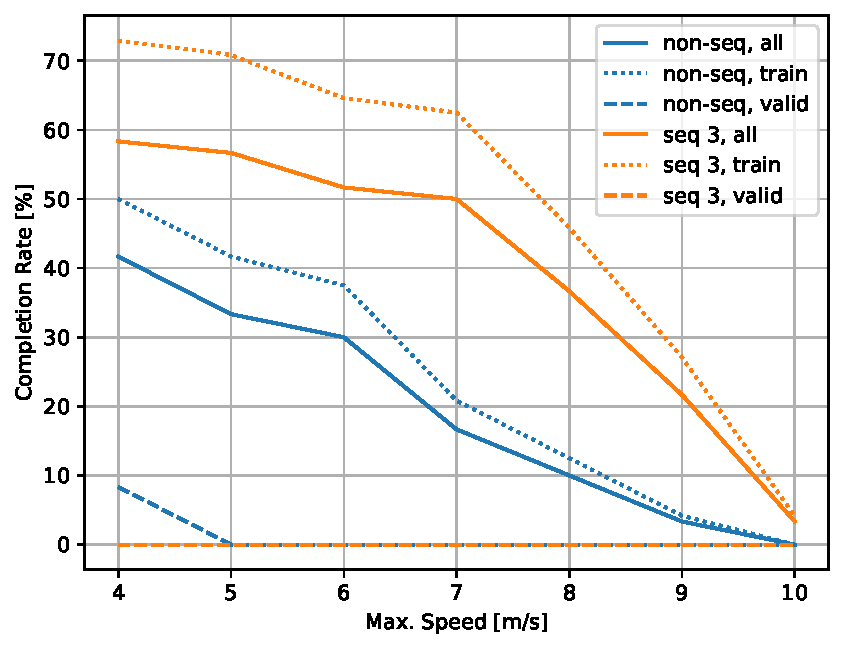
\includegraphics[width=0.9\textwidth]{own/racing_results_0.pdf}
    \caption[
        ???
    ]{
        ???
    \label{fig:?}}
\end{figure}

\begin{figure}
    \centering
    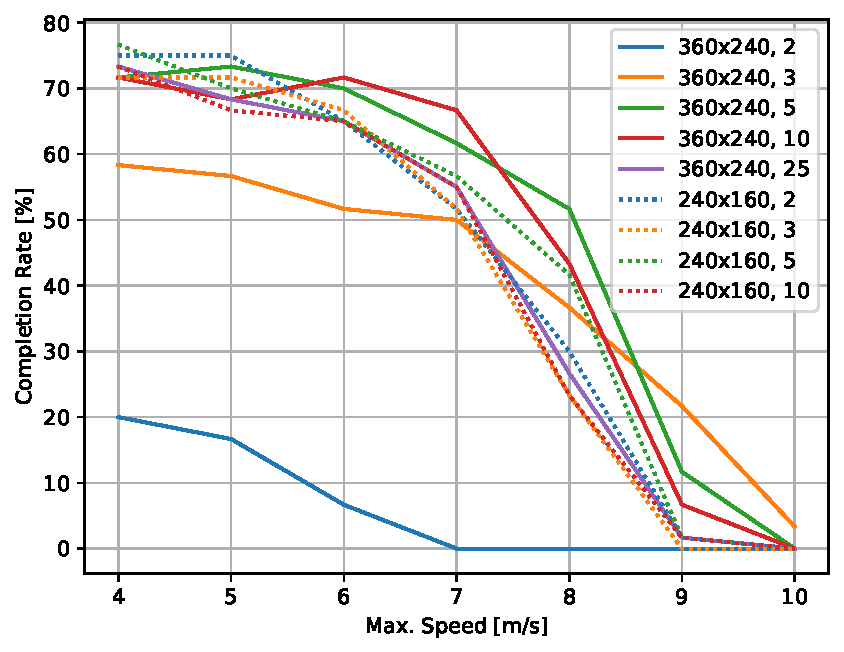
\includegraphics[width=0.9\textwidth]{own/racing_results_1.pdf}
    \caption[
        ???
    ]{
        ???
    \label{fig:?}}
\end{figure}

\begin{figure}
    \centering
    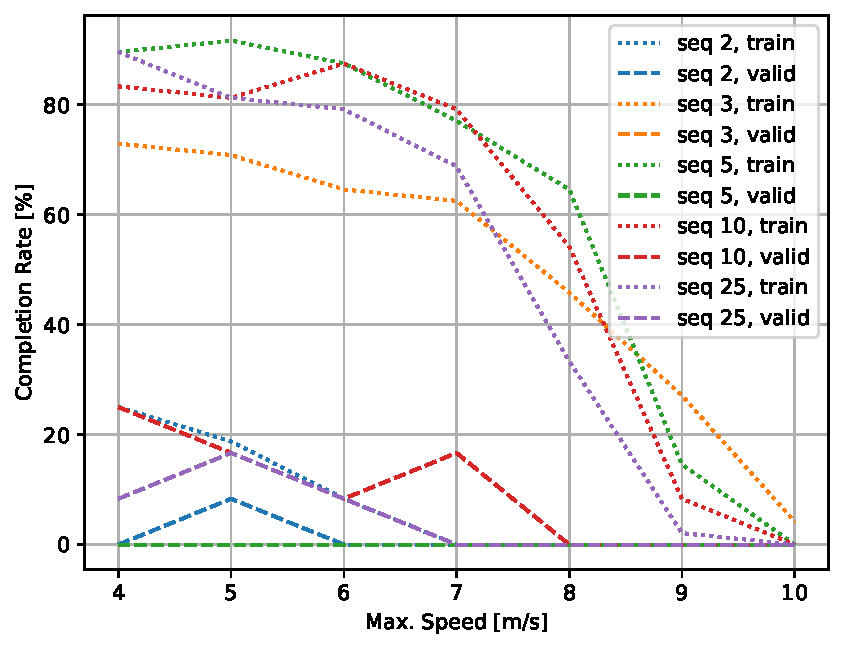
\includegraphics[width=0.9\textwidth]{own/racing_results_2.pdf}
    \caption[
        ???
    ]{
        ???
    \label{fig:?}}
\end{figure}

\begin{figure}
    \centering
    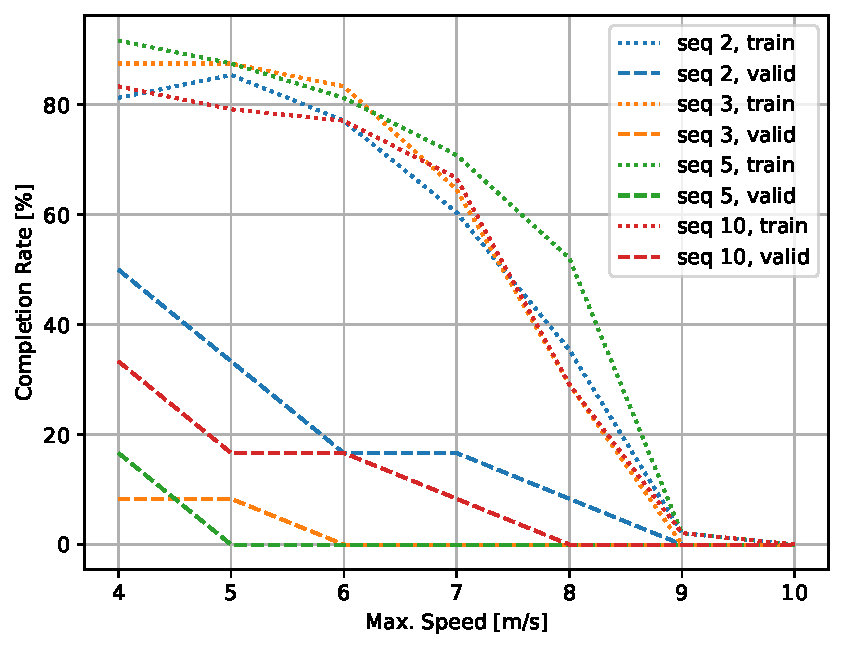
\includegraphics[width=0.9\textwidth]{own/racing_results_3.pdf}
    \caption[
        ???
    ]{
        ???
    \label{fig:?}}
\end{figure}


%###################################################################################
%###################### Discussions         ########################################
%###################################################################################
\section{Discussions}
\label{discussions}
\chapter{Conclusion and Future Work}
\label{conclusion}
%#############################################################
%###################### Summary   ############################
%#############################################################
\section{Summary}
%DELETEME: put a plain summary of your work here. 
%Summaries should be made of each Chapter beginning with Chapter~2 
%and ending with you evaluation. 
%Just write down what you did and 
%describe the corresponding 
%results without reflecting on them.



Chapter \ref{background} provided background information 
on imitation learning with dataset aggregation and the gated recurrent unit (GRU).
The first section presented a definition of the general imitation learning problem
as well as the most intuitive approach to the problem (i.e, behavioral cloning).
Upon this, the more advanced approach of dataset aggregation is presented,
which is applied in the experiments of this thesis.
The second section introduced the class of recurrent neural networks (RNN)
together with the special RNN architecture of the GRU.
This included the state and gating mechanisms of the GRU that can infer from temporal connections in the input
and backpropagation through time, which is used to train the GRU and other RNNs.
Chapter \ref{mainone} presented the autonomous navigation method of the baseline work,
which is used for the experiments of this thesis.
The first section introduced the three reference systems 
and their transformations applied by the modules of the method.
The second section presented the ANN module of this thesis,
which has the function to make navigation decisions based on the RGB images from the drone's onboard camera.
The ANN module comprising the CNN, CAT, FC, GRU and HEAD submodules
is a modularized version of the ANN of the baseline work
that additionally integrates the CAT submodule,
which extends the decision-making basis with the optional inputs
(i.e., the time steps of the images and the estimates from the drone's onboard IMU)
and the GRU submodule,
which extends the decision-making capabilities with temporal comprehension.
The third section presented the planning module of the method,
which has the function to compute local trajectories based on the navigation decisions made by
the ANN module or, in the imitation learning process, the expert system.
The fourth section, presented the control stack of the method,
which has the function to compute the drone's motor inputs 
to track the local trajectories computed by the planning module.
The fifth section presented the expert system of the method,
which in the rollouts of the imitation learning process,
intervenes, whenever the ANN module makes a poor navigation decision.
For every expert intervention in the rollouts, a training sample 
labeled with the expert navigation decision is generated and added to the dataset.
Chapter \ref{maintwo} presented the four experiments of this thesis,
which were all conducted in simulation and investigated different ANN module variants with respect to different aspects.
The first section presented the implementation and the configuration options of the simulation.
The second section presented the process and the configuration options of the imitation learning with dataset aggregation.
The third section presented the process and the configuration options of the race tests.
The following four sections presented the configurations of the four conducted experiments.
Experiment 1 studied two feedforward and three recurrent ANN module variants,
that trained with imitation learning
on the randomized figure-8 racetrack in a single simulation environment
and were tested in the same setting.
Experiment 2 studied several recurrent ANN module variants which 
are configured like the best performing recurrent variant of experiment 1
but differ in their numbers of GRU layers. 
The variants were trained on the dataset aggregated by the best performing variant of experiment 1
and performed the same race tests as in experiment 1.
Experiment 3 studies a feedforward and a recurrent ANN
module variant
that trained with imitation learning
on the randomized gap racetrack in several simulation environments.
The variants performed race tests in the same simulation environments
as well as in simulation environments unseen in the learning process.
Experiment 4 studied several recurrent ANN module variants which 
are configured like the better performing recurrent variant of experiment 3
but differ in the input sequence length of their training samples and 
the input RGB image size.
The variants were trained on the dataset aggregated by that better performing variant of experiment 3
and performed the same race tests as in experiment 3.
Chapter \ref{results} presented the following results of the four experiments,
which were subsequently discussed and interpreted.
In experiment 1, both feedforward variant stalled in the imitation learning process,
while all three recurrent variants could complete it.
The first feedforward variant, which represents the ANN used in the baseline work,
performed by far the most rollouts and aggregated by far the most data.
The second feedforward variant, which integrates a more complex CNN submodule than the first feedforward variant,
performed the second most rollouts and aggregated the second most data.
The first recurrent variant, which is the recurrent counterpart to the second feedforward variant,
performed the least rollouts and aggregated the least data.
The second recurrent variant, that differs from the first recurrent variant by using additional inputs,
performed the second least rollouts and aggregated the second least data.
The third recurrent variant, that differs from the first recurrent variant by the only partly trainable CNN submodule,
performed the third least rollouts and aggregated the third least data.
Both feedforward variant achieved roughly the same final training and validation losses,
which are higher than the final losses of the three recurrent variants.
In the experiment, the first recurrent variant has the fewest final validation loss,
the second recurrent variant has the fewest final training loss
and the highest final validation-training loss ratio,
and the third recurrent variant has the fewest final validation-training loss ratio.
In the race tests,
the first feedforward variant performed by far the worst.
The second feedforward variant performed substantially better.
The first recurrent variant performed by far the best in experiment 1.
Both, the second and the third recurrent variant
perform worse than the first recurrent variant.
In experiment 2, 
the single-layer GRU variant achieves the lowest training
and the highest validation loss.
The ten-layer GRU variant achieves the highest training
and the lowest validation loss.
The variants in between with 2, 3 and 5 GRU layers 
achieve roughly the same training and validation losses.
All variants perform similarly well in the race tests
with the exception of the ten-layer GRU variant,
which performs significantly worse.
In experiment 3, 
the feedforward variant completed the imitation learning process
with less rollouts, less aggregated data 
and a fewer training loss than the recurrent variant.
In environments seen in the imitation learning process,
the recurrent variant clearly outperforms the feedforward variant in the race tests.
In unseen environments, both variants failed the race tests.
In experiment 4,
the variants with the larger image size achieve fewer training losses
than the variants with the smaller image size.
Moreover, the variants with longer input sequence lengths achieve
fewer training losses than the variants with shorter input sequence lengths.
In seen environments,
all variants perform roughly the same in the race tests.
In unseen environments, the variants with the smaller image size performed slightly better
than the variants with the larger image size.










%#############################################################
%###################### Conclusion ###########################
%#############################################################
%DELETEME: do not summarize here. 
%Reflect on the results that you have achieved. 
%What might be the reasons and meanings of these? 
%Did you make improvements in comparison to the state of the art? 
%What are the good points about your results and work? 
%What are the drawbacks? 
\section{Conclusion}
This thesis was motivated by the consideration that when
approaching objects or avoiding obstacles in their immediate environment,
humans rely primarily on their visual perception of their surroundings, 
which is not limited to what is currently in their field of view, 
but also extends to their memory of what they have already seen.
They are able to link this memory to their often subconscious
decisions of how to move to reach a goal,
allowing them to incorporate, for example, 
their own motion history or their estimation and anticipation of how objects move or are likely to move
into their decision-making.
State-of-the-art autonomous navigation methods for drones 
employ CNNs to derive navigation decisions from visual sensor data,
thereby basing decision-making on a high spatial understanding of the drone's current environment.
The objective of this thesis was to investigate the hypothesis
that the combined spatial and temporal comprehension of human navigation
is beneficial for the simplified navigation task of autonomous drone racing.
The approach to this goal was 
to use the autonomous drone racing method of Kaufmann et al. \cite{Kaufmann2018} as a baseline,
to extend the baseline's ANN module responsible for the navigation decision-making,
which consists of a CNN and fully-connected layers,
with the GRU architecture
and finally to evaluate the performance 
of the baseline method for different feedforward and recurrent ANN module variants delivered in simulated experiments.


The experimental results largely support the investigated hypothesis.
In experiment 1 and 3, the recurrent ANN module variant significantly outperformed its feedforward counterpart 
in the race tests, which is especially remarkable for experiment 3
where the recurrent variant has significantly less trainable parameters.
In experiment 1, where the variants have comparable numbers of trainable parameters,
the recurrent variants significantly outperformed the feedforward variants in the imitation learning process,
which is accompanied by significantly fewer rollouts and aggregated data 
as well as significantly lower training and validation losses.
The lower training and validation losses combined with the better or equal race test performance of
the recurrent variants of experiment 1 showed that, first, 
the data aggregated by the recurrent variants, although less, is more comprehensive,
suggesting that navigation decisions are indeed temporally connected 
to past visual observations from the drone's onboard camera
and second, that the recurrent variant can learn to leverage these 
underlying temporal connections for a more accurate and more generalizing navigation decision-making.
in contrast, the feedforward variant, which is by design unable to learn temporal connections,
requires more data for a worse or equal race test performance,
likely because the absence of temporal comprehension makes it 
less robust against intermediate ambigueties of the racetrack 
and outlying visual observations not represented by the aggregated data.
Considering the fewer learning rollouts required,
the recurrent variants are much more advantageous for real-world experiments
where rollouts are more time-consuming, expensive and risky than in simulation.
In experiment 3, a better performance of the recurrent variant on the gap racetrack type 
in unseen environments could have explicitly substantiate the hypothesis.
However, the simulation configuration of the experiment allowed both variants
to evade by learning visual features in the environment.
Experiments 2 and 4 where the variants trained with supervised learning due to time concerns
showed that lower training and validation losses 
do not automatically lead to better performance in race tests, 
emphasizing how important it is for an imitation learning problem
that the state distribution in the aggregated data matches the state distribution during rollout.
The results from both experiments would probably substantially differ 
if the variants were trained with imitation learning.
However, the fact the variants could fit the precollected data more accurately,
the longer the input sequence length of the data was,
again emphasizes the existence of temporal connections in the navigation decision-making.

None of the examined variants could keep up with the strong, experimental results of the baseline work.
The reason for this is likely that the experiments in the baseline work 
were conducted on another racetrack layout, 
which is less challenging to the autonomous navigation method,
in a non-photorealistic simulation,
which due to less details and variations simplifies visual perception.
A more stringent imitation learning configuration,
resulting in more aggregated data,
could possibly achieve comparable results,
however, would also have made the imitation learning processes even more time-intensive.
A disadvantage of the recurrent variants is that the training epochs on sequential data
is much more time-consuming than on non-sequential data.
Even if the training epochs of the recurrent variants are more effective
and thus less epochs per rollout are required,
the imitation learning process tends to be longer than for feedforward variants,
if they do not stall as in experiment 1.

The experiments were only conducted in simulation.
It remains open, if the recurrent variants could outperform the feedforward variants also in the real world
in the light of greater visual detailedness and stronger disturbances.
Problems could arise with a too long inference time of the variants running
on a drone with restricted computational power. However, the MAC numbers and the observations in simulation
indicate that the feedforward and recurrent variants have roughly the same inference time.
A drawback of this thesis is that the experimental design is somewhat unstructured,
since the experiments naturally emerged in the debugging process of the
implementation of the recurrent variants and its learning process.
Many preliminary tests were conducted,
in which it was yet unclear whether the baseline method and the ANN module
were implemented correctly
and whether the recurrent variants
with the different operation modes of many-to-one at training 
and one-to-one at rollouts is able to learn at all.
Moreover, there were a variety of user-specifiable parameters to consider,
which complicated the design of the experiments.



%The time expenditure of the imitation learning is anyhow the biggest drawback of the baseline method,
%which became particularly noticable because the experiments were conducted on my personal computer.
%From my today's perspective, it was a mistake to chose this topic for my master thesis
%since I totally lacked the content and hardware related support. The research environment for this thesis 
%was me, myself and I locked in my home office.
%This made the whole thesis and especially the designs of the experiments somewhat unstructered,
%since the experiments naturally emerged in the debugging process of the recurrent variants,
%in which due to absent content-related feedback I was unsure, for example, 
%if the recurrent variants
%with the different operation modes of many-to-one at training and one-to-one at rollouts can learn at all.
%However, even if the 
%hypothesis only one navigation method, only in simulation (inference time)
%- wirre vorangehensweise (personal computer) longer sequences








%#############################################################
%###################### Future Work ##########################
%#############################################################
\section{Future Work}
The simulated experiments of this thesis were conducted under the restrictions of the COVID-19 pandemic 
with the minimal resources of my student home office.
They could show that the use of a CNN-GRU architecture
significantly increases the performance of the baseline method 
in the imitation learning process and in the race tests.
Embedded in a research environment that allows for more vibrant scientific discourse 
and provides more computationally powerful hardware, 
the following open questions could be investigated.


Experiment 1 considered only a single simulation environment
and in experiment 3, the variants learned in environments in only four different scenes
and failed the race tests in the environments of the fifth scene unseen in the learning process.
Further experiments where the variants learn in more numerous and diverse environments
could investigate whether the variants can generalize to environments unseen in the learning process
and whether the feedforward and the recurrent variant differ in their generalization abilities.
In experiment 3 the variants learned visual clues in the environments to navigate the gap of the racetracks.
More tailored experiments, where the variants learn in a monochrome environment absent of visual clues,
could investigate whether the recurrent variants can learn to navigate the gap only with the help of their memory abilities.
In Experiment 2 and 4, the variants trained only with supervised learning.
Further experiments could conduct these two experiments with imitation learning,
which would produce more meaningful results regarding the impact of the
GRU submodule's configuration and memory time span
induced by the input sequence length of the training samples.
The race test performances in the simulated experiments of the baseline work are much better than
in the experiments of this thesis where the test conditions were more difficult.
Further experiments with more comparable test conditions
could verify or falsify the results of the baseline work 
or could identify reasons for the performance difference.
All experiments of this thesis were conducted in simulation.
The question remains open, whether the results could be transfered to real-world experiments.

In this thesis, temporal comprehension in the navigation decision-making
was realized with the GRU architecture.
The deployment of other recurrent architectures such as the
more prevalent long short-term memory (LSTM) LINK or the more recent
Content Adaptive Recurrent Unit (CARU)
\url{https://link.springer.com/chapter/10.1007/978-3-030-63830-6_58}
could be investigated.
In this thesis, the imitation learning problem was solved with dataset aggregation,
where the recurrent variants learned better than the feedforward variants.
Further experiments where the imitation learning problem is solved with inverse reinforcement learning,
could compare the learning performance of recurrent and feedforward variants for this type of imitation learning.
Other autonomous drone racing methods or even more general autonomous navigation methods
could be used as baselines to investigate whether temporal comprehension only improves the baseline method 
of this thesis or is generally useful in autonomous navigation.




%DELETEME: Regarding your results - which problems did you not solve? 
%Which questions are still open? 
%Which new questions arised? 
%How should someone / would you continue working in your thesis field basing on your results?
---^
\begin{itemize}
    \item \url{https://en.wikipedia.org/wiki/Gated_recurrent_unit#Content-Adaptive_Recurrent_Unit}
    \item \url{https://en.wikipedia.org/wiki/Gated_recurrent_unit#Architecture}
\end{itemize}


%__________________________End_of_Thesis______________________________________________
\cleardoublepage
\addcontentsline{toc}{chapter}{Bibliography}
%harvard citations style, please uncomment harvard package in the usepackage area
%\bibliographystyle{agsm}
%remove the following line when using harvard style citation
\bibliographystyle{plain}
%specify bibtex file here
\bibliography{input/mybib}
%add appendix to TOC
\addcontentsline{toc}{chapter}{Appendices}
\chapter*{Appendices}
\label{appendices}
DELETEME: everything that does not fit into your work, e.g. a 5 page table that breaks the reading flow, should be placed here

%###################################################################################
%###################### Appendix A          ########################################
%###################################################################################
%uncomment, if desired
%\newpage
\addcontentsline{toc}{section}{Appendix A: Abbreviations}
\section*{Appendix A: Abbreviations}
\begin{center}
\begin{tabular}{ll}
\textbf{AES}	&	Advanced Encryption Standard (Symmetrisches Verschl�sselungsverfahren)\\
\textbf{ASCII}&	American Standard Code for Information Interchange (Computer-Textstandard)\\
\textbf{dpi}	&	dots per intch (Punkte pro Zoll; Ma� f�r Aufl�sung von Bilddateien)\\
\textbf{HTML}	&	Hypertext Markup Language (Textbasierte Webbeschreibungssprache)\\
\textbf{JAP}	&	Java Anon Proxy\\
\textbf{JPEG}	&	Joint Photographic Experts Group (Grafikformat)\\
\textbf{JPG}	&	Joint Photographic Experts Group (Grafikformat; Kurzform)\\
\textbf{LED}	&	Light Emitting Diode (lichtemittierende Diode)\\
\textbf{LSB}	&	Least Significant Bit\\
\textbf{MD5}	& Message Digest (Kryptographisches Fingerabdruckverfahren)\\
\textbf{MPEG}	&	Moving Picture Experts Group (Video- einschlie�lich Audiokompression)\\
\textbf{MP3}	&	MPEG-1 Audio Layer 3 (Audiokompressionformat)\\
\textbf{PACS}	&	Picture Archiving and Communication Systems\\
\textbf{PNG}	&	Portable Network Graphics (Grafikformat)\\
\textbf{RSA}	&	Rivest, Shamir, Adleman (asymmetrisches Verschl�sselungsverfahren)\\
\textbf{SHA1}	&	Security Hash Algorithm (Kryptographisches Fingerabdruckverfahren)\\
\textbf{WAV}	&	Waveform Audio Format (Audiokompressionsformat von Microsoft)\\
%\textbf{abk}	&	erkl�rung\\
%\textbf{abk}	&	erkl�rung\\
%\textbf{abk}	&	erkl�rung\\
%\textbf{abk}	&	erkl�rung\\
%\textbf{abk}	&	erkl�rung\\
%\textbf{abk}	&	erkl�rung\\
%\textbf{abk}	&	erkl�rung\\
%\textbf{abk}	&	erkl�rung\\
%\textbf{abk}	&	erkl�rung\\
%\textbf{abk}	&	erkl�rung\\
%\textbf{abk}	&	erkl�rung\\
%\textbf{abk}	&	erkl�rung\\
%\textbf{abk}	&	erkl�rung\\
\end{tabular}
\end{center}

%###################################################################################
%###################### Appendix B          ########################################
%###################################################################################
\newpage
%change this
\addcontentsline{toc}{section}{Appendix B: {\LaTeX} Help}
\section*{Appendix B: {\LaTeX} Help}
%remove this
\subsection*{How to Use This Template}
\begin{itemize}
\item Remove all of my text which is mostly labeled with DELETEME
\item Change the information in the 00a\_title\_page.tex file
\item Use the information written in this section
\item Ask you supervizor to help you
\item If I am not your supervizor and noone else can help you, write me an email (aubrey.schmidt@dai-labor.de)
\end{itemize}

%###################################################################################
%###################### Citations           ########################################
%###################################################################################
\subsection*{Citations}
Citing is one of the essential points you need to do in you thesis. Statements not basing on results of your own research\footnote{in what ever context} not being cited represent a breach on the rules of scientific working. Therefore, you every statement needs to be cited basing on information that other people can cross-check. A common way of citing in technical papers is: 
\begin{itemize}
\item Oberheide et al.~\cite{oberheide:2008:cloudav} state that the average time for an anti-virus enginge to be updated with a signature to detect an unknown threat is 48 days.
\end{itemize}
Note: et al. is used when the paper was written by more than two people. Check the code of this section to learn how to cite from a technical perspective.

Note: you can change the citation style in the \texttt{thesis.tex} file, e.g. to harvard style citations. Instructions on this can also be found in this file.

You should not cite anything that can be changed, e.g. it is not that good citing web pages since they might get updated changing the cited content. There are no clear quality measures on citing sources but aubrey believes that the following list is true for several cases, starting with highest quality:
\begin{enumerate}
\item Journal article or book
\item Conference paper
\item Workshop paper
\item Technical report
\item Master thesis
\item Bachelor thesis
\item General Web reference
\end{enumerate}
There might be workshop papers that have a higher quality than some journal papers. Therefore this list only gives you a hint on possible quality measures. Another measure can be whether a paper was indexed by ACM/IEEE, although this is not a strong indicator.

%###################################################################################
%###################### Papers             ########################################
%###################################################################################
\subsection*{Finding and Handling Citation Sources}
Following ressources are required for finding and handling articles, books, papers and sources.
\begin{itemize}
\item your primary resource will be \url{http://scholar.google.com}
\item \url{http://www.google.com} might also be used
\item \url{wikipedia.com} can be a good start for finding relevant papers on your topic
\item you should download and install JabRef or a similar tool \url{http://jabref.sourceforge.net/}
\item you should point JabRef to the mybib.bib file
\item you should immediately enter a relevant paper to JabRef, additionally, you should write a short summary on it; else, you will do this work at least twice.
\end{itemize}

%###################################################################################
%###################### General             ########################################
%###################################################################################
\subsection*{General Advices}
\begin{itemize}
\item Do not take care of design, \LaTeX will do this for you. If you still feel that you need to take care of this, do this when you have finished writing, else you will end up in a lot of double and triple work.
\item \LaTeX will do exactly that you will tell it to do. If you have problems with this, go for google or ask you supervizor
\item use labels in order to be able to reference to chapters, section, subsections, figures, tables, etc. ...
\end{itemize}

%###################################################################################
%###################### Commands            ########################################
%###################################################################################
\subsection*{General Commands}
\begin{itemize}
\item check \url{http://en.wikibooks.org/wiki/LaTeX}
\item check \url{http://www.uni-giessen.de/hrz/tex/cookbook/cookbook.html} German
\end{itemize}
Please also check the following source~\cite{latexcookbook2007}.

%###################################################################################
%###################### Code                ########################################
%###################################################################################
\newpage
\subsection*{Code}
This section shows you how to get your code into a \LaTeX document. See code for options.
\lstinputlisting[language=JAVA,xleftmargin=8mm,]{__help/Example.java}


\lstset{ %
language=Java,   	             % the language of the code
numbers=left,
basicstyle=\scriptsize,       % the size of the fonts that are used for the code
numbers=left,                   % where to put the line-numbers
numberstyle=\scriptsize,      % the size of the fonts that are used for the line-numbers
stepnumber=1,                   % the step between two line-numbers. If it's 1, each line 
                                % will be numbered
numbersep=5pt,                  % how far the line-numbers are from the code
backgroundcolor=\color{white},  % choose the background color. You must add \usepackage{color}
showspaces=false,               % show spaces adding particular underscores
showstringspaces=false,         % underline spaces within strings
showtabs=false,                 % show tabs within strings adding particular underscores
frame=single,                   % adds a frame around the code
tabsize=2,                      % sets default tabsize to 2 spaces
captionpos=b,                   % sets the caption-position to bottom
breaklines=true,                % sets automatic line breaking
breakatwhitespace=false,        % sets if automatic breaks should only happen at whitespace
title=\lstname,                 % show the filename of files included with \lstinputlisting;
                                % also try caption instead of title
xleftmargin=8mm,
framexleftmargin=4mm,           
escapeinside={\%*}{*)},         % if you want to add a comment within your code
morekeywords={*,...}            % if you want to add more keywords to the set
}
\begin{lstlisting}[float=h, caption=Example code is presented here, label=list:code, frame=single]
class Beispiel{

	public static void main(String args[]){
	
		System.out.println("Hello World");
		
	}
	
}
\end{lstlisting}

%###################################################################################
%###################### Figures             ########################################
%###################################################################################
\newpage
\subsection*{Figures}
This section describes how to include images to your document. Information was taken from \url{http://en.wikibooks.org/wiki/LaTeX/Floats,_Figures_and_Captions}, visited on 05/08/2011. Please make sure to use original vector graphics as basis since image quality might be used as weak indicator for thesis quality. For this, try to find find files in \texttt{.SVG} or \texttt{.PDF} format. Exporting a \texttt{.PNG} or \texttt{.JPG} to \texttt{.PDF} will not work since data was already lost while exporting it to these formats. This is the case for most Web graphics. Wikipedia startet entering most in images in \texttt{.SVG} which easily can be transformed to \texttt{.PDF}, but please do not forget proper citations.

%use a modifier to decide where you desire Latex should put the image: (h)ere, (t)op, (b)ottom, or nothing more than that image on a (p)age
\begin{figure}[h]%[htbp]
%this will center your image
\centering
%this will include your image
\includegraphics[width=0.15\textwidth]{template/TUBerlin_Logo_rot_hell}
%this is the caption + label. the label will not be printed in the caption. Moving the label out of the caption can result in problems.
\caption[Including an Image]{Including an image; in this case a PDF. Please note that the caption is placed below the image.\label{fig:help1}}
\end{figure}

\begin{figure}[h]
%this will center your image
\centering
%this will include your image

\includegraphics[width=0.25\textwidth]{template/aot_logo}
%this is the caption + label. the label will not be printed in the caption. Moving the label out of the caption can result in problems.
\caption[Short caption for list of figures]{See code for caption options: this is a long caption which is printed in the Text. Additionally, image size was increased\label{fig:help2}}
\end{figure}


\begin{figure}[h]
  \centering
  \subfloat[Small]{\label{fig:tub1}\includegraphics[width=0.1\textwidth]{template/TUBerlin_Logo_rot_hell}}                
  \subfloat[Large]{\label{fig:tub2}\includegraphics[width=0.3\textwidth]{template/TUBerlin_Logo_rot_hell}}
  \subfloat[Medium]{\label{fig:tub3}\hspace{2cm}\includegraphics[width=0.2\textwidth]{template/TUBerlin_Logo_rot_hell}}
  \caption[Placing images side by side]{Placing images side by side using the subfig package. Space between the images can be adjusted.\label{fig:tuball}}
\end{figure}


%###################################################################################
%###################### Tables              ########################################
%###################################################################################
\newpage
\subsection*{Tables}
Here, you will find some example tables.The tables were taken from \url{http://en.wikibooks.org/wiki/LaTeX/Tables}, visited on 05/08/2011. Table environment was added plus caption and label. For code, check \url{__help/latex_hinweise.tex}.

\begin{table}[h]
\caption{Simple table using vertical lines. Note that the caption is always above the table! Please check code for finding the right place for the table label.\label{tab:help1}}
\centering
  \begin{tabular}{ l | c || r | }
    \hline
    1 & 2 & 3 \\ \hline
    4 & 5 & 6 \\ \hline
    7 & 8 & 9 \\
    \hline
  \end{tabular}
\end{table}

\begin{table}[h]
\caption{Table using vertical and horizontal lines\label{tab:help2}}
\centering
\begin{tabular}{|r|l|}
  \hline
  7C0 & hexadecimal \\
  3700 & octal \\ \cline{2-2}
  11111000000 & binary \\
  \hline \hline
  1984 & decimal \\
  \hline
\end{tabular}
\end{table}

\begin{table}[h]
\caption{Table with column width specification on last column\label{tab:help3}}
\centering
    \begin{tabular}{ | l | l | l | p{5cm} |}
    \hline
    Day & Min Temp & Max Temp & Summary \\ \hline
    Monday & 11C & 22C & A clear day with lots of sunshine.  
    However, the strong breeze will bring down the temperatures. \\ \hline
    Tuesday & 9C & 19C & Cloudy with rain, across many northern regions. Clear spells
    across most of Scotland and Northern Ireland,
    but rain reaching the far northwest. \\
    \hline
    \end{tabular}
\end{table}

\begin{table}[h]
\caption{Table using multi-column and multirow\label{tab:help4}}
\centering
\begin{tabular}{|l|l|l|}
\hline
\multicolumn{3}{|c|}{Team sheet} \\
\hline
Goalkeeper & GK & Paul Robinson \\ \hline
\multirow{4}{*}{Defenders} & LB & Lucus Radebe \\
 & DC & Michael Duberry \\
 & DC & Dominic Matteo \\
 & RB & Didier Domi \\ \hline
\multirow{3}{*}{Midfielders} & MC & David Batty \\
 & MC & Eirik Bakke \\
 & MC & Jody Morris \\ \hline
Forward & FW & Jamie McMaster \\ \hline
\multirow{2}{*}{Strikers} & ST & Alan Smith \\
 & ST & Mark Viduka \\
\hline
\end{tabular}
\end{table}







\end{document}
